% This text is proprietary.
% It's a part of presentation made by myself.
% It may not used commercial.
% The noncommercial use such as private and study is free
% Sep. 2005 
% Author: Sascha Frank 
% University Freiburg 
% www.informatik.uni-freiburg.de/~frank/


\documentclass[notes]{beamer}
\usepackage[utf8]{inputenc}
\usetheme{Madrid}
\useoutertheme{noslidenum}
\usepackage{graphicx}
\usepackage{verbatim}
\usepackage{xcolor}
\usepackage{amsmath}
\usepackage{siunitx}
%\usepackage{amssym}
%%\usepackage[spanish]{babel}
\graphicspath{{./figs/}}
\renewcommand{\parallel}{{\mkern3mu\vphantom{\perp}\vrule depth 0pt\mkern2mu\vrule depth 0pt\mkern3mu}}
\let\oldhat\hat
\renewcommand{\vec}[1]{\mathbf{#1}}
\renewcommand{\hat}[1]{\oldhat{\mathbf{#1}}}

%%%%%%%%%%%%%%%%%%%%%%%
% NOTAS
%%%%%%%%%%%%%%%%%%%%%%%
\usepackage{pgfpages}
\setbeameroption{show notes on second screen}

\AtBeginSection[] {
  \begin{frame}[plain]
    \frametitle{Contents}
    \tableofcontents[currentsection]
  \end{frame}
  %\addtocounter{framenumber}{-1}
} 

\begin{document}
\titlegraphic{
\includegraphics[width=2cm]{logos/logo-UBA.png}\hspace*{1.875cm}~%
   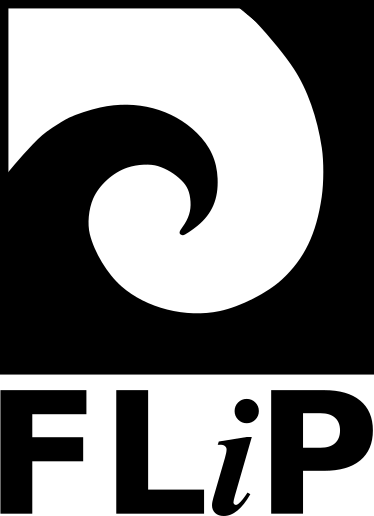
\includegraphics[width=1cm]{logos/flip_logo.png}\hspace*{1.875cm}~%
   
\includegraphics[width=2cm]{logos/logo-CONICET.png}
 }
\title[Defensa tesis doctoral]{Comportamiento espacio-temporal de
turbulencia magnetohidrodinámica}
\author[]{Rodrigo Lugones\\Director: Pablo A. Dmitruk}

\institute[]{Universidad de Buenos Aires, Grupo de Fluidos y Plasmas, IFIBA-CONICET}
%\date{\today}
\date{6 de marzo de 2020}

\frame{\titlepage} 

%\frame{\frametitle{Contents}\tableofcontents} 

\frame{\frametitle{Resumen}
\begin{itemize}
\item En esta tesis estudiamos algunos de los aspectos fundamentales
  de la turbulencia MHD, tales como la transferencia espectral de
  energía o la multiplicidad de escalas temporales presentes.
\item Analizamos el comportamiento espacio-temporal de los campos
  magnético y de velocidades estudiando el espectro de energías y los
  tiempos de descorrelación. Esto nos permite distinguir el efecto
  físico dominante en una amplia variedad de situaciones.
\item Analizamos los espectros espacio-temporales de los campos de
  Elsässer, variando independientemente el campo magnético medio y la
  helicidad cruzada.
\end{itemize}
}


%\section{Introduction}

\frame{\frametitle{Marco general}
El mayor porcentaje de la materia visible en el espacio y en sistemas
astrofísicos se encuentra en estado de plasma.\vfill

La dinámica de los plasmas espaciales (como el viento solar) puede mostrar
grandes diferencias en sus propiedades físicas con respecto a los plasmas
de laboratorio.\vfill

Una mayor comprensión de los efectos físicos presentes en los plasmas
espaciales permite, entre otras cosas, un mayor entendimiento del
medio interplanetario.\vfill

  \begin{columns}
    \column{0.4\textwidth}
    \begin{minipage}[t]{1\textwidth}
      \begin{center} 
        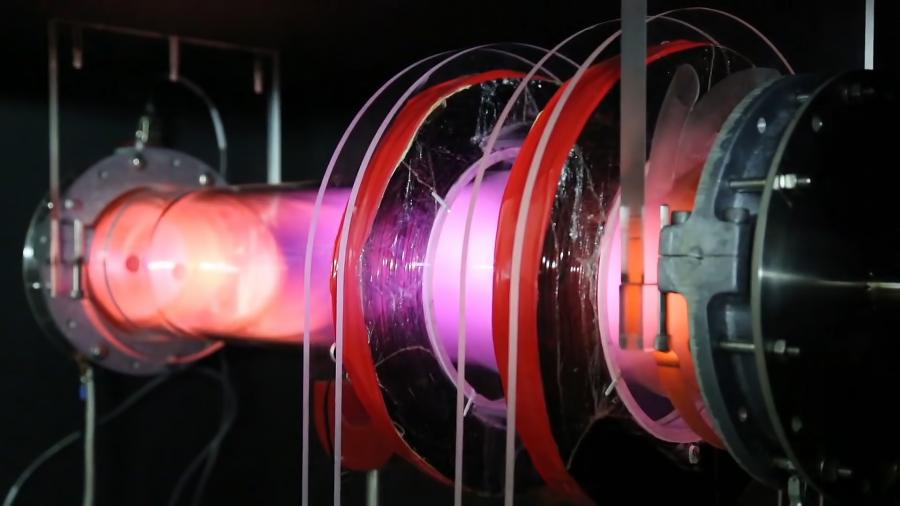
\includegraphics[width=\columnwidth]{extra/plasma2.jpg}
      \end{center}
    \end{minipage}
    \column{0.6\textwidth}
    \begin{minipage}[t]{1\textwidth}
      \begin{center}
        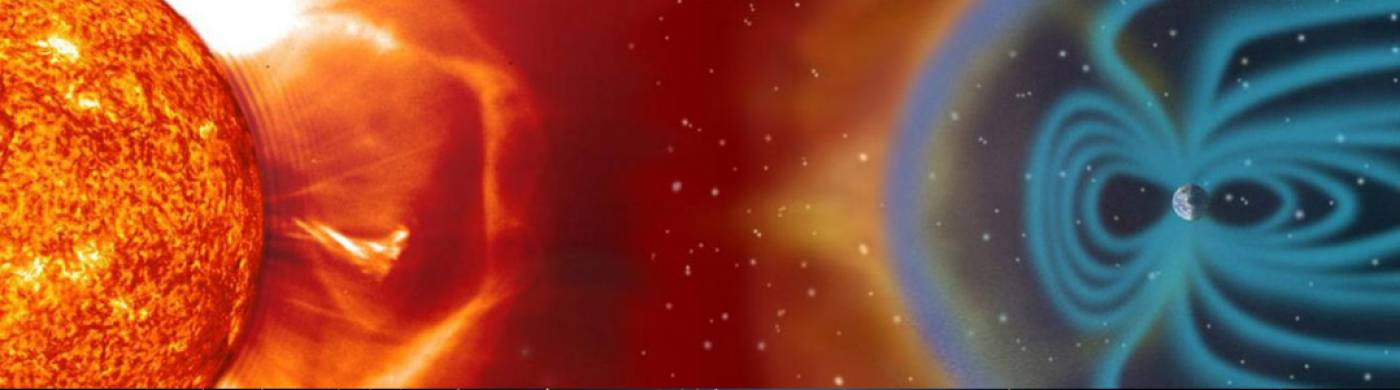
\includegraphics[width=\columnwidth]{extra/plasma1.jpg}
      \end{center}
    \end{minipage}
  \end{columns}
}
\note[itemize]{
\item DE QUÉ SIRVE LO QUE ESTUDIAMOS?
\item
\item 1) Fluido conductor que evoluciona con fuerzas Mec y EM.
\item 2) Baja colisión, baja densidad, alta velocidad alta temperatura.
\item Todo esto, arma un panorama complejo
\item
\item SIGUIENTE: MÁS COMPLEJO. TURBULENCIA.
}


\frame{\frametitle{Marco general}
  \begin{columns}
    \column{0.7\textwidth}
    \begin{minipage}[t]{1\textwidth}
Para complejizar la cuestión, en el caso del viento solar, se desarrolla
un regimen turbulento en su expansión por el medio interplanetario.
    \end{minipage}
    \column{0.3\textwidth}
    \begin{minipage}[t]{1\textwidth}
      \begin{center}
        \includegraphics[width=\columnwidth]{extra/plasma3.png}
      \end{center}
    \end{minipage}
  \end{columns}\vfill

  \begin{columns}
    \column{0.4\textwidth}
    \begin{minipage}[t]{1\textwidth}
        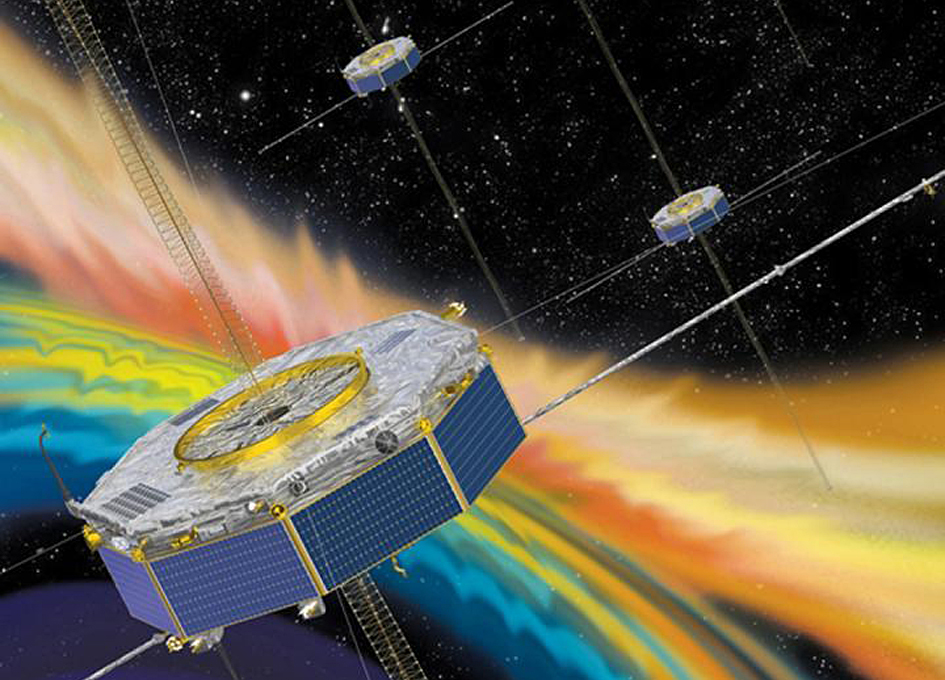
\includegraphics[width=\columnwidth]{extra/plasma4.jpg}
    \end{minipage}
    \column{0.6\textwidth}
    \begin{minipage}[t]{1\textwidth}
      \begin{flushright}
Sin embargo, hay cada vez más mediciones \emph{in situ} proporcionadas
por misiones espaciales.
      \end{flushright}
    \end{minipage}
  \end{columns}
}
\note[itemize]{
\item
\item SIGUIENTE: CÓMO SE DESCRIBE PLASMA
}


\frame{\frametitle{?`Cómo describir físicamente el plasma?}
En líneas generales, existen tres grandes enfoques posibles:
\begin{itemize}
\item Movimiento individual de las partículas.
\item Descripción cinética de una colección de partículas.
\item Descripción fluidística: magnetohidrodinámica (MHD)
\end{itemize}
La descripción MHD de un fluido describe adecuadamente la
fenomenología a grandes escalas temporales y espaciales.
}
\note[itemize]{
\item 1) $6N$ (esp fases), $N\sim 10^{15}$ en $\SI{1}{km^3}$ en medio interplanetario.
\item 2) Con funciones de distribución para cada especie, satisfaciendo ecuaciones cinéticas (como Vlasov).
\item 3) N-S con Maxwell
\item MHD se puede complejizar: dos fluidos, Hall-MHD, electron-MHD
\item Trabajaremos con MHD-1fluido con \textbf{turbulencia}
\item
\item ENTRA TURBULENCIA
}


\frame{\frametitle{Marco general}
Al igual que en el caso HD, en MHD la turbulencia introduce caos y aleatoriedad.\vfill

Algunos de los parámetros estadísticos calculables son los tiempos de
descorrelación y los espectros energéticos.\vfill

A lo largo de la presente charla, estudiaremos las correlaciones eulerianas temporales
y los espectros espacio-temporales.





}
\note[itemize]{
\item 1) Sin embargo, no de cualquier manera.
\item 1) Hay muchos parámetros estadísticos que permiten describir al plasma.
\item
\item 3) Desc lagrangiana: asociado a transferencia energética.
\item 3) Desc euleriana: predicciones limitantes.
  Está relacionada con diversos fenómenos (por ej, intermitencia).
\item 3) Las correlaciones espaciales y temporales proveen información acerca
  de la distribución espacial y temporal de la energía a lo largo de distintas escalas.
}


\frame{\frametitle{Un poco de turbulencia HD}
\begin{equation*}\label{eq2:N-S}
  \frac{\partial \vec{v}}{\partial t} + \vec{v}\cdot\nabla\vec{v} =
  -\frac{1}{\rho}\nabla p + \nu\nabla^2 \vec{v},
\end{equation*}

\begin{itemize}
\item Viscosidad presente $\Rightarrow$ decaimiento energético distintivo
\item Taylor, von Karman, Howarth, Kolmogorov.
\end{itemize}

  \begin{columns}
    \column{0.5\textwidth}
    \begin{minipage}[t]{1\textwidth}
      \begin{center} 
        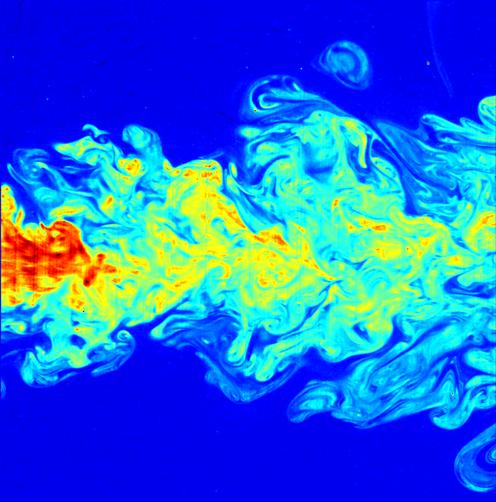
\includegraphics[width=0.6\columnwidth]{extra/turbulence1.jpg}
      \end{center}
    \end{minipage}
    \column{0.5\textwidth}
    \begin{minipage}[t]{1\textwidth}
      \begin{center}
        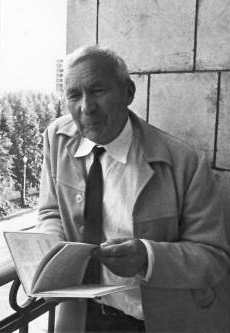
\includegraphics[width=0.5\columnwidth]{extra/turbulence2.jpg}
      \end{center}
    \end{minipage}
  \end{columns}
}
\note[itemize]{
\item Turbulencia MHD $\neq$ HD.
\item $B$ de gran escala juega rol significativo.
\item Influencia pequeñas escalas.
\item Entonces más escalas temporales influenciando.
\item Entonces, cascada más compleja
\item
\item Sin embargo, HD vale la pena como intro.
\item
}




\frame{\frametitle{Un poco de turbulencia HD}
El proceso de transferencia de energía:
\begin{center}
  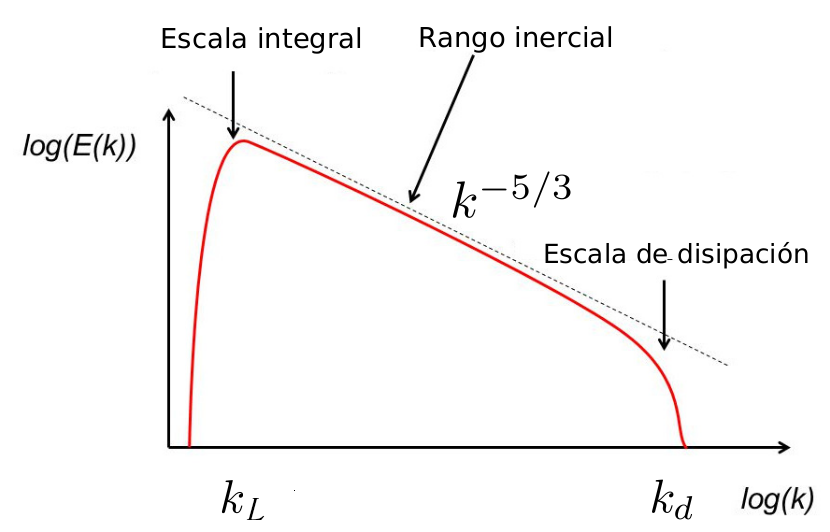
\includegraphics[width=0.4\columnwidth]{Fundamentos/EspectroKolmogorov.png}
\end{center}

Para poder inferir el espectro en el rango inercial, es necesario
estimar la magnitud de las correlaciones de la función de
transferencia (triple correlación), y en consecuencia la escala
temporal del decaimiento de las correlaciones de las funciones de
transferencia, $\tau_T(k)$.\vfill

Por argumentos dimensionales, $\epsilon = \overline{C} \tau_T(k) k^4 E^2(k)$. \vfill

El espectro de Kolmogorov, $E(k) = C_K \epsilon^{2/3} k^{-5/3}$, se
recupera proponiendo $\tau_T(k) = \tau_{nl}(k)$, donde este último
tiempo es el tiempo característico de los \emph{eddies}, $\tau_{nl}(k)
= \ell/v_k$.
}
\note[itemize]{
\item Fuerza aplicada a escala $L$ (ingresa energía)
\item Movimiento inestable y pierde energía a escalas vecinas más pequeñas, sin disiparse directamente en forma de calor
(transferencia local de energía).
\item Proceso repetido hasta escala de disipación $l_d$ (la escala de Kolmogorov), donde la
energía transferida se dispersa en forma de calor por acción
viscosa.
\item
\item EFECTOS. STRAINING Y SWEEPING.
}


\frame{\frametitle{Un poco de turbulencia HD: \emph{straining} y \emph{sweeping}}
\begin{itemize}
\item El espectro de Kolmogorov clásico se basa en la representación de la cascada
energética, causada por la interacción de \emph{eddies} de casi el mismo tamaño.
\item Las interacciones consisten en movimientos de \underline{\emph{straining}}.
\item También está presente la interacción entre escalas grandes y pequeñas, mediante
un movimiento de barrido (\underline{\emph{sweeping}}), pero no involucra transferencia energética
significativa en el espacio de Fourier.
\item En las correlaciones temporales, el \emph{sweeping} cobra gran importancia.
\item También cobra importancia para los momentos de orden más alto.
\end{itemize}
}
\note[itemize]{
\item 1) Cascada energética, similar a saltos de agua.
\item 2) Un vórtice se estira, produciendo grad de velocidades que distorsiona otros vórtices.
\item 3) Los remolinos grandes arrastran a los pequeños, pero no los deforman.
\item 4) \emph{Frozen turbulence}
\item 5) Funciones de estructura, espectro de energía cinética, etc.
\item 5) Entonces, no influye el espectro, pero es importante.
\item
\item AGREGARSE EFECTOS EXTRA
}


\frame{\frametitle{Un poco de turbulencia HD}
Ahora bien, ?`cómo pueden agregarse los efectos de otras escalas
temporales en una teoría simple de espectros turbulentos? Una
posibilidad es reescribir la tasa de transferencia espectral:
$\epsilon = \Pi(k) = \frac{u_k^2}{\tau_{sp}}$\vfill

Aquí, el tiempo de transferencia espectral de energía puede escribirse
como $\tau_{sp} = \tau_{nl}^2/\tau_T(k)$. Desarrollando diferentes
aproximaciones para $\tau_T$ de la triple correlación, es posible
obtener una variedad de modelos para los espectros de turbulencia.\vfill

%% Es más, este enfoque fenomenológico concuerda con las conclusiones de
%% las diversas teorías de clausura de la turbulencia: la ley espectral
%% de potencias viene determinada por la elección de una escala temporal
%% relacionada con las transferencias no lineales de energía.

Resulta razonable buscar un tratamiento fenomenológico del espectro
MHD para entender la variedad de conclusiones que pueden ser
aplicables al espacio y a plasmas astrofísicos.
}
\note[itemize]{
\item 2) Esto se condice con conclusiones de las teorías de clausura.
\item
\item TURBULENCIA MHD
}




\frame{\frametitle{Turbulencia MHD}
\begin{center}
$\frac{\partial \vec{v}}{\partial t} + \vec{v} \cdot \nabla\vec{v} = -\frac{1}{\rho} \nabla p + \frac{1}{4\pi\rho} \left(\nabla\times\vec{B}\right)\times\vec{B} + \nu \nabla^2 v$ \\
$\frac{\partial \vec{B}}{\partial t} = \nabla \times \left(\vec{v}\times\vec{B}\right) + \mu \nabla^2 \vec{B}$
\end{center}\vfill

El modelo MHD es frecuentemente aplicado al espacio y a plasmas
astrofísicos. \vfill

Cuando se tienen observaciones experimentales
disponibles (viento solar), se puede ver que el rango inercial es
amplio, por lo que el rango de inyección de energía se encuentra bien
separado en escala del rango disipativo, y resulta posible inferir un
Reynolds efectivo.
}
\note[itemize]{
\item Ecs. de momentos y de inducción magnética
}



\frame{\frametitle{Turbulencia MHD}
\begin{itemize}
\item El campo magnético puede ser escrito como $\vec{B} = \vec{B}_0 + \vec{b}$.
\item El campo magnético de gran escala permite y respalda la propagación de ondas
hidromagnéticas (ondas de Alfv\'en).
\item Estas ondas son fluctuaciones transversales a $\vec{B}_0$, propagándose
en su misma dirección a la velocidad de Alfv\'en $V_A =
B_0/\sqrt{4\pi\rho}$, y siguiendo la relación de dispersión $\omega
= \pm V_A k_\parallel$.
\item Las fluctuaciones de pequeña escala sufren un efecto
similar al \textit{sweeping} debido a la propagación de ondas de
Alfv\'en (\textit{sweeping} magnético).
\item Además, el \emph{sweeping} juega un papel importante, pues
$\vec{B}_0$ no puede ser removido por transformaciones de Galileo $\Rightarrow$ anisotropía.
\item Esto introduce una nueva escala temporal, complejizando la turbulencia.
\end{itemize}
}
\note[itemize]{
\item 1) Parte uniforme $\vec{B}_0$ (DC) o que varía muy suavemente
(campo magnético medio local), más fluctuaciones de pequeña escala $\vec{b}$
\item
\item TEORÍAS FENOMENOLÓGICAS
}





\frame{\frametitle{Turbulencia MHD}
Hay varias teorías fenomenológicas, dependiendo de la escala temporal dominante:
\begin{itemize}
\item Iroshnikov (1964) y Kraichnan (1965): $\tau_T = \tau_A \Rightarrow E(k) \sim k^{-3/2}$
\item Fyfe y Montgomery (1976): $\tau_T = \tau_{nl} \Rightarrow E(k) \sim k^{-5/3}$
\item Matthaeus y Zhou (1989): $\frac{1}{\tau_T(\vec{k})} = \frac{1}{\tau_{nl}(\vec{k})} + \frac{1}{\tau_A(\vec{k})}$
\end{itemize}
}
\note[itemize]{
\item $\tau_T(k)$: escala temporal del decaimiento de las correlaciones
de las funciones de transferencia.
\item I-K: Para $B_0$ fuerte.
\item F-M: Vale Kolmogorov
\item M-Z: Respeta los casos límites
}



\frame{\frametitle{Turbulencia MHD}
Más allá de los detalles (presentes en la tesis), la conclusión es que
con MHD el análisis se complejiza aún más.\vfill

En cualquier caso, las distintas escalas temporales tienen un rol
influyente en la transferencia de energía, las cascadas, la no
localidad y la anisotropía.\vfill

Los movimientos de \textit{straining} son dominantemente locales en
escala, dado que las distorsiones no lineales son más efectivas para
interacciones entre \textit{eddies} de aproximadamente el mismo
tamaño.\vfill

Por su parte, el barrido debido a propagación de ondas Alfv\'enicas
introduce un nuevo nivel de no-localidad en MHD y una fuerte tendencia
a que la transferencia espectral ocurra anisotrópicamente respecto de
la dirección del campo magnético.
}
\note[itemize]{
\item
\item ESPECTROS DE FRECUENCIAS
}



\frame{\frametitle{Espectros de frecuencias}
\begin{itemize}
\item En los '70, la investigación de la turbulencia hidrodinámica
se dirigió al estudio del tiempo de descorrelación del campo de
velocidades.
\item Además de las correlaciones espaciales, también cobró interés el estudio del
espectro en frecuencias más allá de la hipótesis de Taylor.
\item La conclusión principal fue que el \textit{sweeping} aleatorio domina
la descorrelación temporal en el rango inercial para el caso hidrodinámico.
\end{itemize}
}
\note[itemize]{
\item 2) correlaciones de dos tiempos y un punto espacial
}


\frame{\frametitle{Espectros de frecuencias}
\begin{itemize}
\item Nuevamente, el caso MHD resulta mucho más complejo, quedando aún
muchas preguntas acerca de cuál es la escala temporal dominante de la
descorrelación temporal.
\item Servidio \emph{et al} (2011) realizaron un estudio para
analizar a descorrelación temporal para el caso de turbulencia MHD
isotrópica.
\item El resultado principal: la descorrelación temporal en MHD es gobernada por
interacciones no locales, pero no pudieron
distinguir entre los efectos del \emph{sweeping} y de la distorsión
Alfv\'enica.
\end{itemize}
\begin{center}
  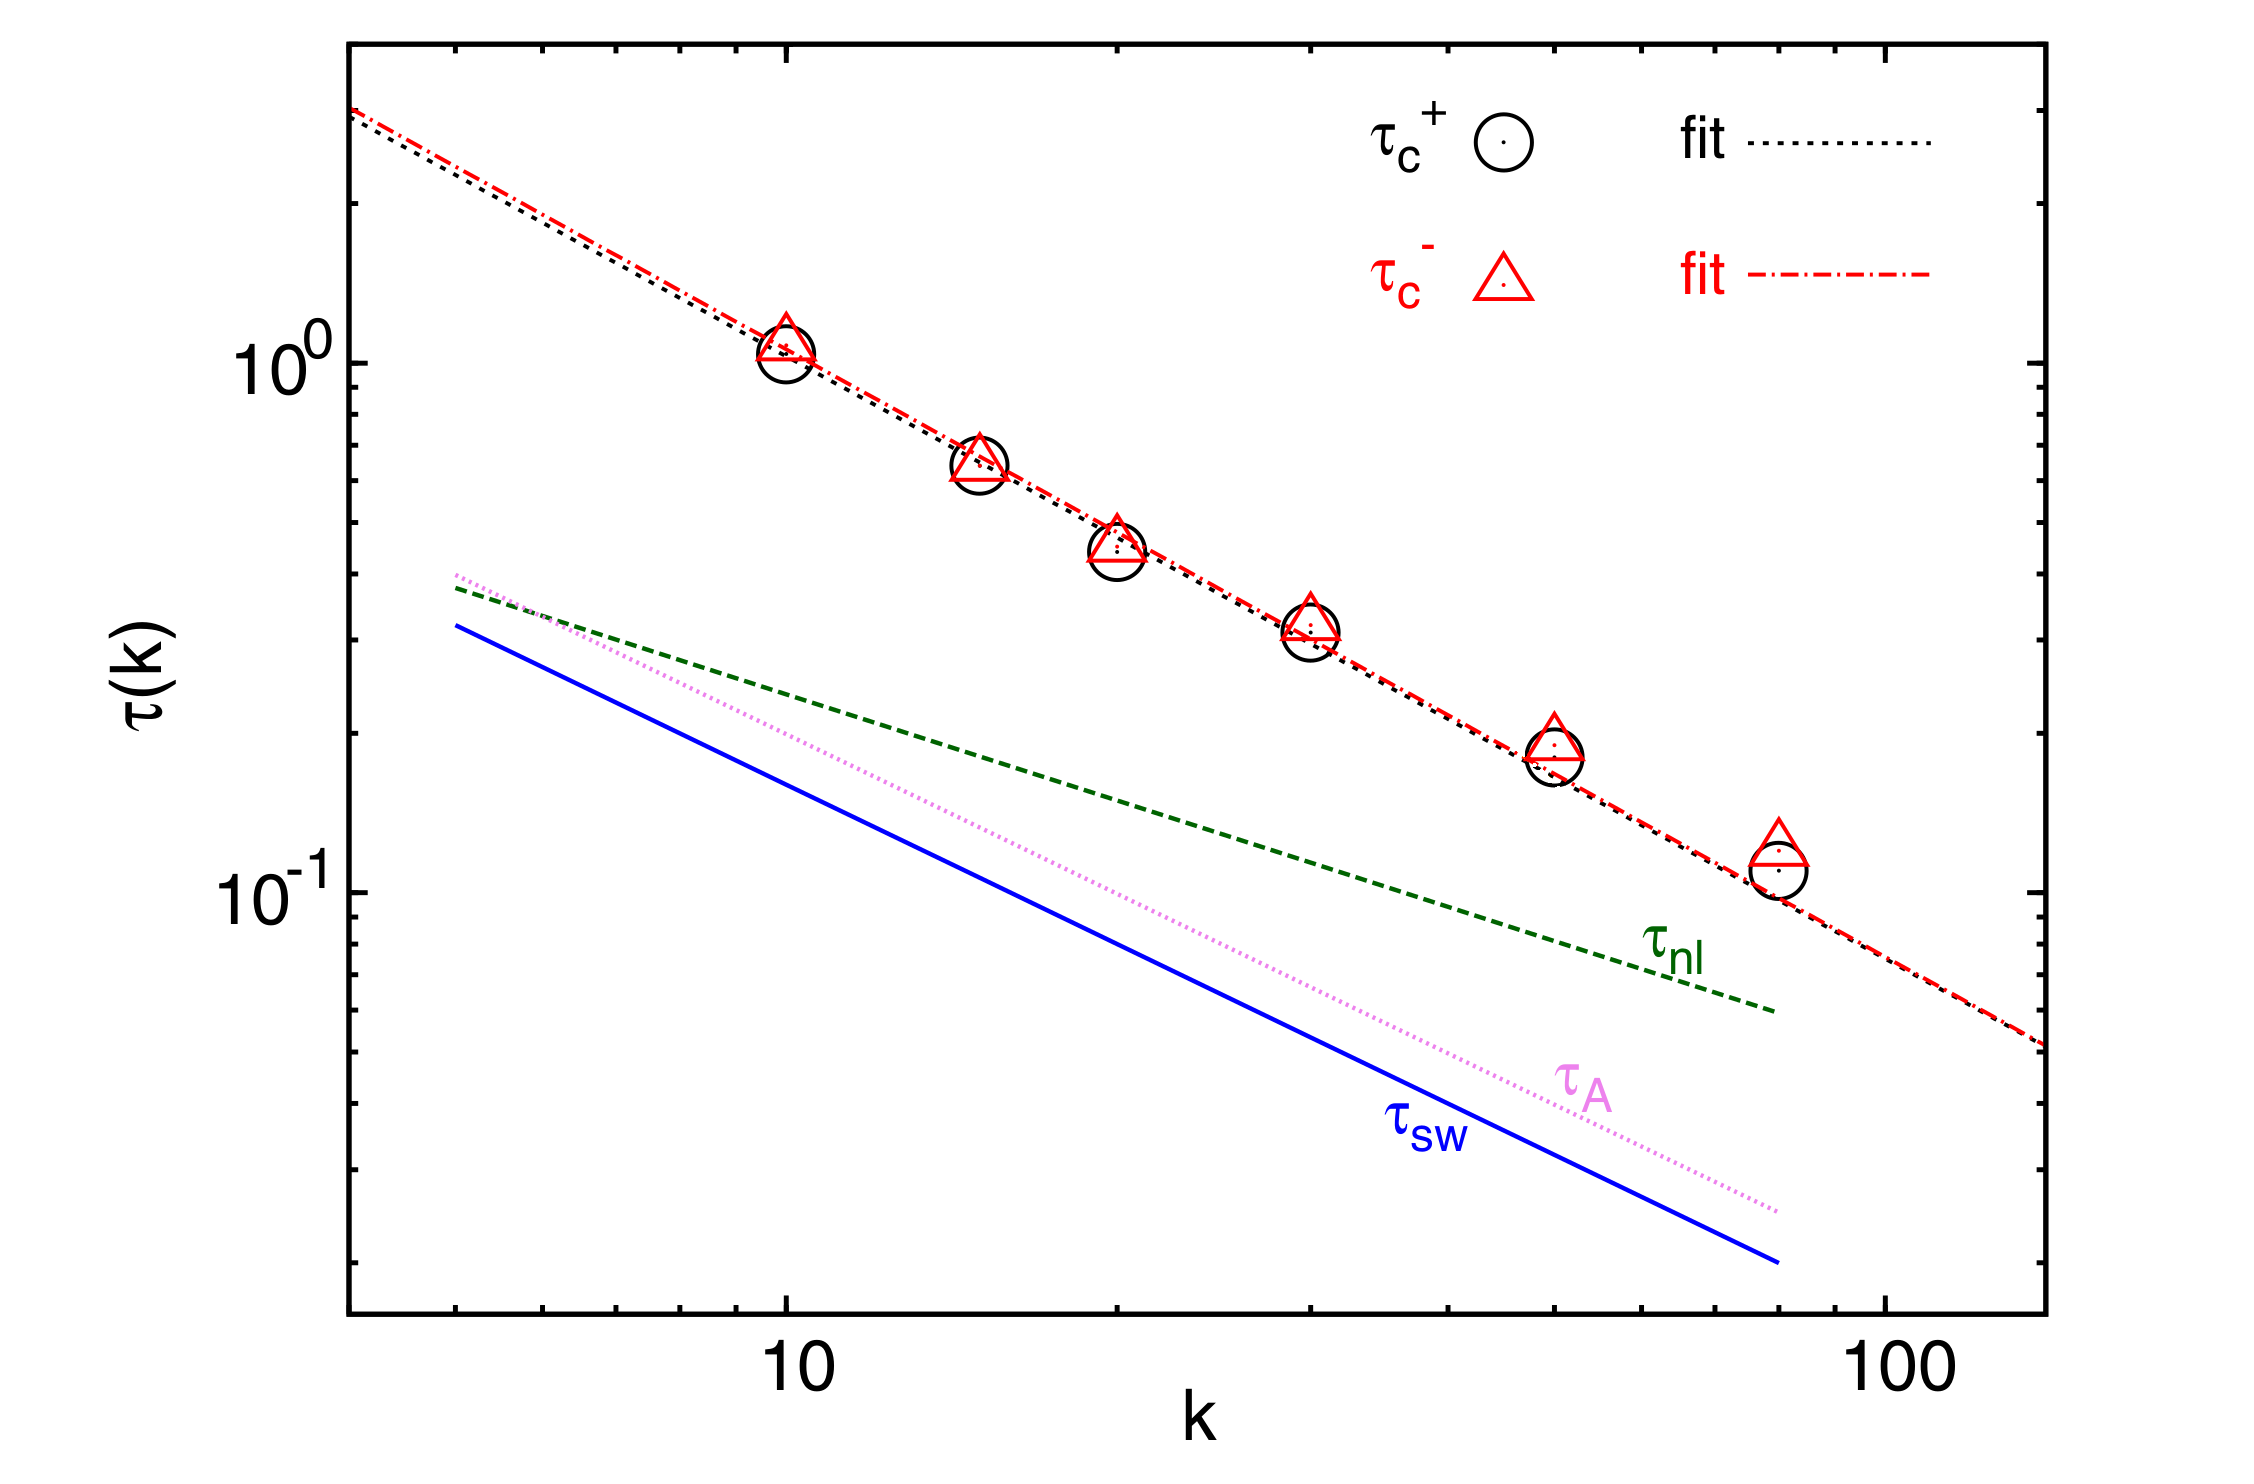
\includegraphics[width=0.4\columnwidth]{Fundamentos/ServidioDescorrelacion.png}
\end{center}
}
\note[itemize]{
\item 2) en este caso, \emph{sweeping} aleatorio y propagación de Alfv\'en
\item figura: tiempos de decorrelación
\item
\item CASO DE ESTUDIO
}


\frame{\frametitle{Caso de estudio}
  \begin{itemize}
  \item El caso más simple corresponde a MHD incompresible con un
    campo magnético $\vec{B_0}$ de fondo, para el cual la relación de
    dispersión lineal $\omega = \vec{k}\cdot\vec{V_A}$ describe ondas
    de Alfv\'en, con $\vec{V_A} = \vec{B_0}/\sqrt{4\pi/\rho}$.
  \item Las escalas temporales pertinentes serán el tiempo no
    lineal $\tau_{nl}$ y las asociadas
    con los efectos no lineales dependientes de la escala, el
    \emph{sweeping} no local ($\tau_{sw}$) y la propagación de ondas de Alfvén ($\tau_A$).
  \end{itemize}
}
\note[itemize]{
\item
\item OBJETIVOS
}







%%%%%%%%%%%%%%%%%%% ANTES
%% \frame{\frametitle{Introducción}
%%   \begin{itemize}
%%   \item Al comienzo de los 70's, las investigaciones de turbulencia
%%     hidrodinámica concluyeron que el \emph{sweeping} domina la
%%     descorrelación temporal en el rango inercial.
%%   \item Recientemente, Servidio \emph{et al} (2011) estudiaron el caso
%%     MHD. Concluyeron que, para el caso de turbulencia isotrópica, la
%%     descorrelación temporal en MHD está gobernada por las
%%     interacciones no locales, pero no pudieron distinguir entre los
%%     efectos de \emph{sweeping} y las distorsiones de Alfv\'en.
%%   \end{itemize}
%% }

%\section{Objectives}
\frame{\frametitle{Objetivos}
  \begin{itemize}
  \item Generalizar el estudio hecho por Servidio a plasmas
    magnetizados a grandes escalas, donde vale la aproximación MHD.
  \item Estudiar y entender la descorrelación temporal de las
    fluctuaciones.
  \item De esta manera, poder diferenciar entre los efectos no
    lineales, de \emph{sweeping} y de Alfv\'en.
  \item Clark di Leoni \emph{et al} (2014) propusieron considerar las
    fluctuaciones a más de una escala en un flujo rotante, para
    discernir entre los diferentes fenómenos asociados a la
    descorrelación temporal.
  \end{itemize}
}

%\section{Equations and numerical simulations}
\frame{\frametitle{Las ecuaciones MHD}
  \begin{equation*}\label{eq:MHD_v}
    \frac {\partial {\bf v}}{\partial t} +
    {\bf v }\cdot \nabla {\bf v} = -\frac{1}{\rho}\nabla p +
    {\bf j} \times {\bf B} + \frac{1}{R} \nabla^2{\bf v} + \vec{F}_v
  \end{equation*}
  \begin{equation*}\label{eq:MHD_b}
    \frac{\partial {\bf b}}{\partial t} = \nabla \times ({\bf v} \times {\bf B})
    + \frac{1}{R_m} \nabla^2 {\bf b} + \vec{F}_b
  \end{equation*}
  \begin{itemize}
    \item ${\bf B} = {\bf b} + {\bf B_0}$, con una parte fluctuante ${\bf
        b}$ y un campo medio DC ${\bf B_0}=B_0\hat{x}$
    \item Las unidades se basan en una velocidad característica, la
      velocidad de Alfv\'en de las fluctuaciones del campo magnético,
      $v_0 = \sqrt{\langle b^2 \rangle /(4\pi\rho)}$.
    \item $R$ y $R_m$ son los números de Reynolds cinético y magnético.
    \item La unidad temporal es $t_0 = L/v_0$, el tiempo de cruce
      Alfv\'enico basado en las fluctuaciones de campo magnético.
  \end{itemize}
}
\note[itemize]{
\item Forzados
\item
\item TIEMPOS CARACTERÍSTICOS
}


%\subsection{Characteristic times}
\frame{\frametitle{Tiempos característicos}
\begin{block}{Tiempo no lineal}
  \begin{itemize}
    \item Local eddy turnover.
  \end{itemize}
  \begin{equation*}
    \tau_{nl} \sim \left[ k v(k) \right]^{-1} \Rightarrow \tau_{nl} \approx \left [ v_{rms} L^{-1/3} \left(\sqrt{k^2_\perp + k^2_\parallel}\right)^{2/3}\right ]^{-1}
  \end{equation*}
\end{block}
\begin{block}{Tiempo de \emph{sweeping}}
  \begin{itemize}
    \item Advección de estructuras de pequeña escala por el flujo de gran escala. 
  \end{itemize}
  \begin{equation*}
    \tau_{sw} \approx \left( v_{rms}\sqrt{k^2_\perp + k^2_\parallel} \right)^{-1}
  \end{equation*}
\end{block}
\begin{block}{Tiempo de Alfv\'en}
  \begin{equation*}
    \tau_A \approx \left( B_0 k_\parallel \right)^{-1}
  \end{equation*}
\end{block}
}
\note[itemize]{
\item A partir de las ecuaciones MHD, salen los tiempos característicos
\item Faltan las constanted $C_i \sim 1$
\item
\item FUNCIONES DE CORRELACIÓN
}



%\subsection{Decorrelation function}
\frame{\frametitle{Función de correlación}
  \begin{itemize}
  \item La estadística de un campo (por ej, el magnético) puede ser
    caracterizada por la función de autocorrelación espacio-temporal a
    dos puntos, $R(\vec{r},\tau) = \left\langle \vec{b}(\vec{x},t)
    \cdot \vec{b}(\vec{x}+\vec{r},t+\tau) \right\rangle / \left\langle
    \vec{b}^2 \right\rangle$
  \item Transformando Fourier en $r$ conduce a una densidad espectral
    temporalmente retrasada $S(\vec{k}, \tau) =
    S(\vec{k})\Gamma(\vec{k},\tau)$
  \item $\Gamma(\vec{k},\tau)$ representa los efectos dinámicos de
    descorrelación que describen la descorrelación de tiempo de cada
    modo espacial $\vec{k}$.
  \item $\Gamma(\vec{k},\tau)$ es la función de correlación temporal
    para $\vec{k}$.
  \item En presencia de un campo guía, $\Gamma = \Gamma(\vec{k}_\perp,
    \vec{k}_\parallel, \tau)$ ayuda a entender la dinámica en
    distintas regiones del espacio de Fourier.
  \end{itemize}
}
\note[itemize]{
\item 5) Esto nos da información acerca de cómo la memoria en una
    dirección afecta a la otra, y de cómo podemos distinguir entre el
    \emph{sweeping} aleatorio y la propagación de Alfv\'en.
\item
\item SIMULACIONES
}



%\subsection{Numerical simulations}
\frame{\frametitle{Simulaciones numéricas}
  \begin{itemize}
    \item Código pseudoespectral estándar que resuelve numéricamente
      las ecuaciones 3D-MHD con un campo guía.
    \item Runge-Kutta de segundo orden como esquema de integración temporal.
    \item \emph{Aliasing} removido con el método de truncamiento de la
      regla de los dos-tercios.
    \item Condiciones de contorno periódicas.
    \item Tamaño de la caja de $2\pi L$, donde $L=1$ es la longitud de
      correlación inicial de todas las fluctuaciones.
    \item $N^3 = 512^3$ puntos de grilla..
    \item $B_0 = 0$, $0.25$, $1$, $4$ y $8$, en unidades del valor
      \emph{rms} inicial de las fluctuaciones magnéticas.
    \item Forzado en la banda $0.9 \leq k \leq 1.8$, con componentes
      aleatorias y temporalmente coherentes ($\tau_f \sim 1$).
  \end{itemize}
}
\note[itemize]{
\item Sakura. 9 nodos 224 clusters.
\item Tardan $\sim 1$ mes.
\item Pesan 1GB
}


%\section{Results}
%\subsection{Energy spectra and dominant time scales}
\frame{\frametitle{Algunos resultados obtenidos...}
  
}


\frame{\frametitle{Espectros de energía y escalas de tiempo dominantes}
  Espectros energéticos perpendiculares reducidos
  \begin{center}
    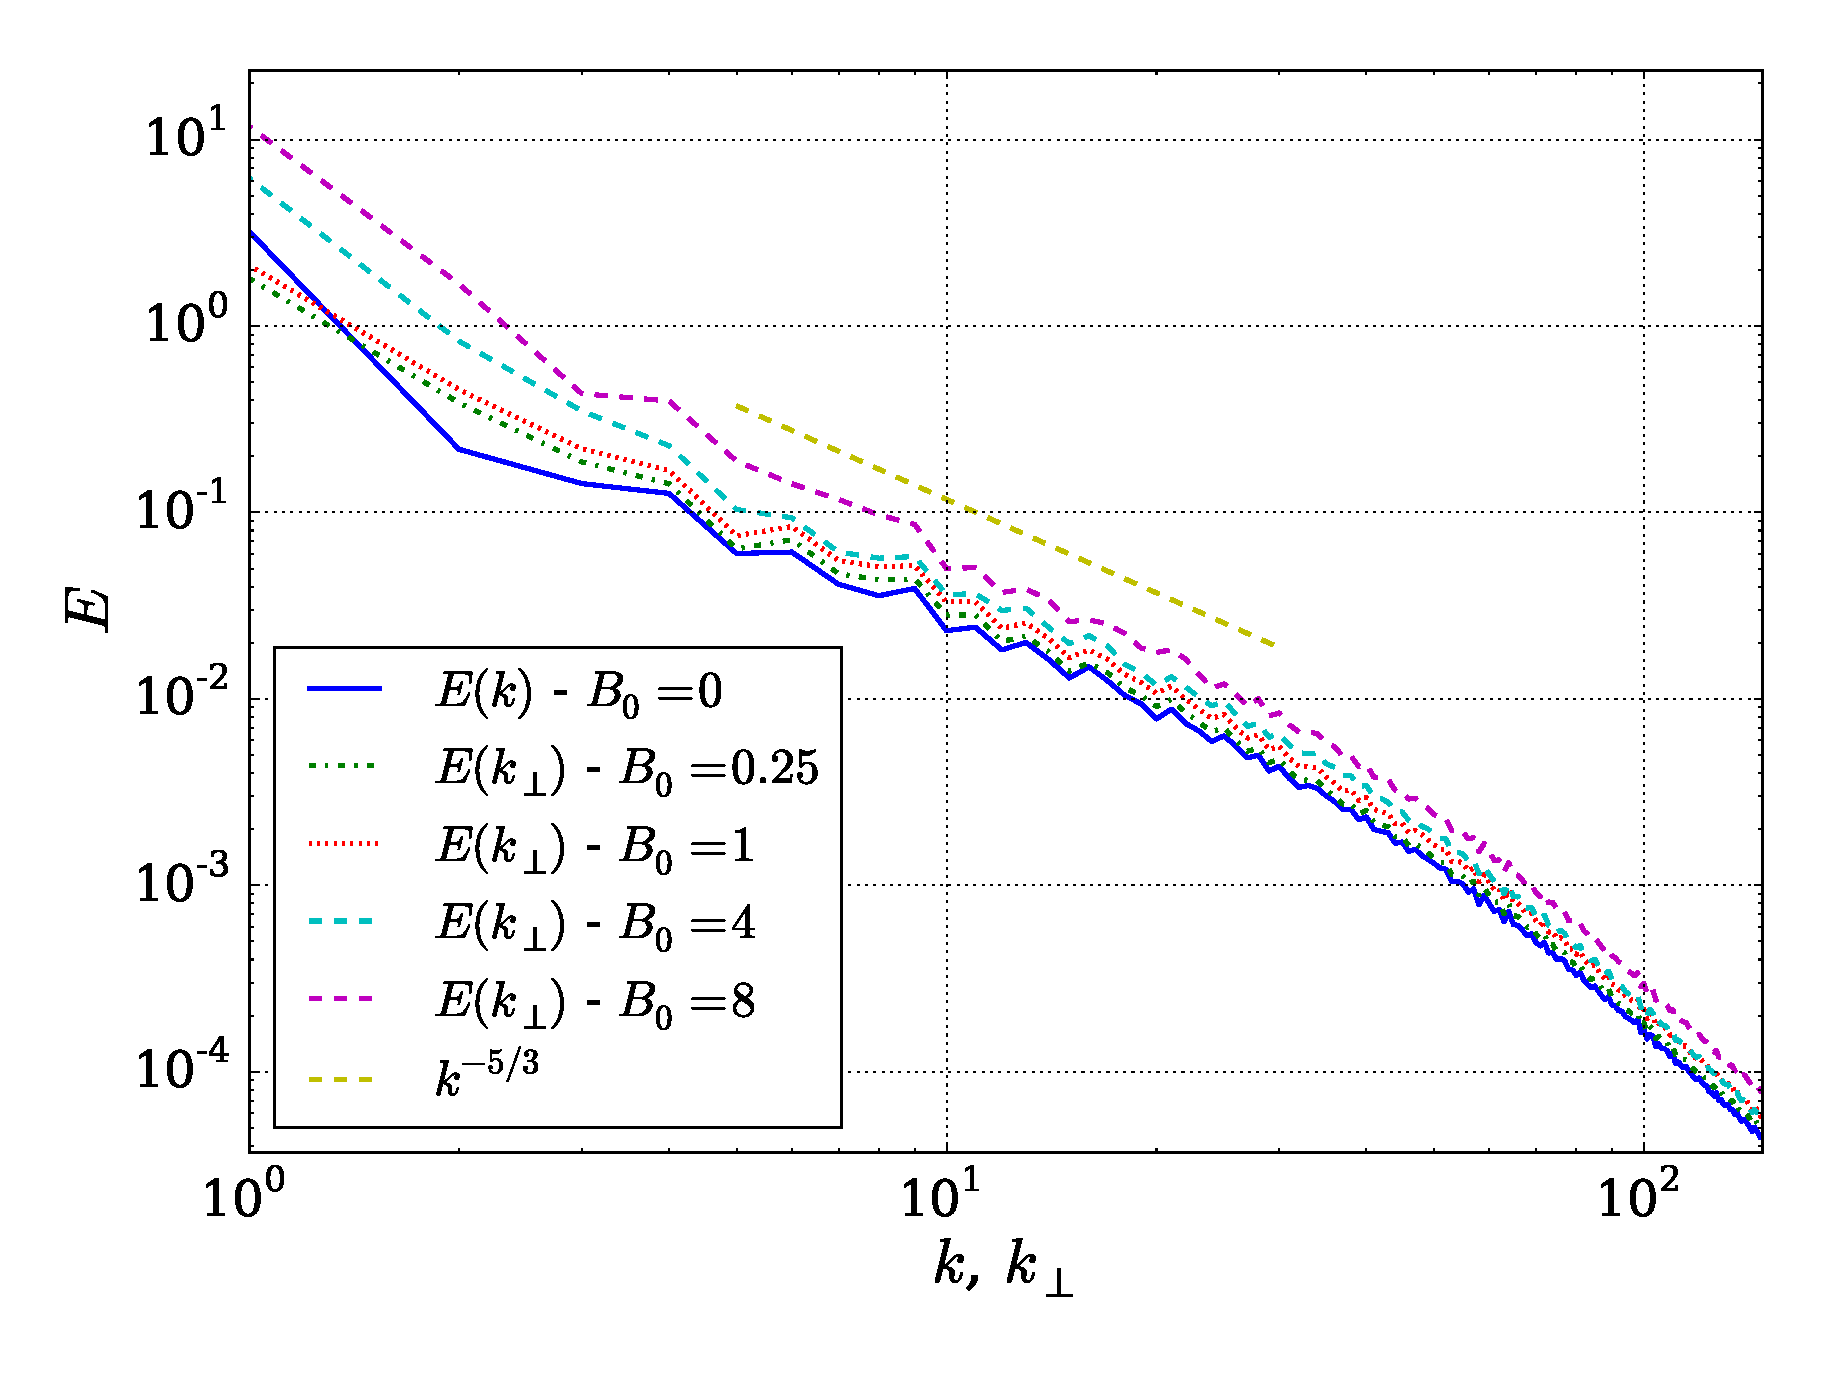
\includegraphics[width=0.7\columnwidth]{P1/fig1_E.eps}
  \end{center}
}
\note[itemize]{
\item Es, básicamente, la energía en función de $k_\perp$.
\item
\item Espectro energético perpendicular reducido y promediado
  temporalmente: $E\left(k_\perp\right) = \frac{1}{T}\int\int
  e(|\vec{k_\perp}|, k_\parallel, t) \, dk_\parallel~dt$
\item Se calcula a partir del espectro axisimétrico.
\item
\item ESPECTRO AXISIMÉTRICO. ENERGÍA EN FUNC DE KPARA Y KPERP

}


\frame{\frametitle{Espectros de energía y escalas de tiempo dominantes}
  \underline{Isocontornos del espectro axisimétrico de energía}
  \pause
  {\Large : $B_0 = 0$}\\
  \begin{center}
    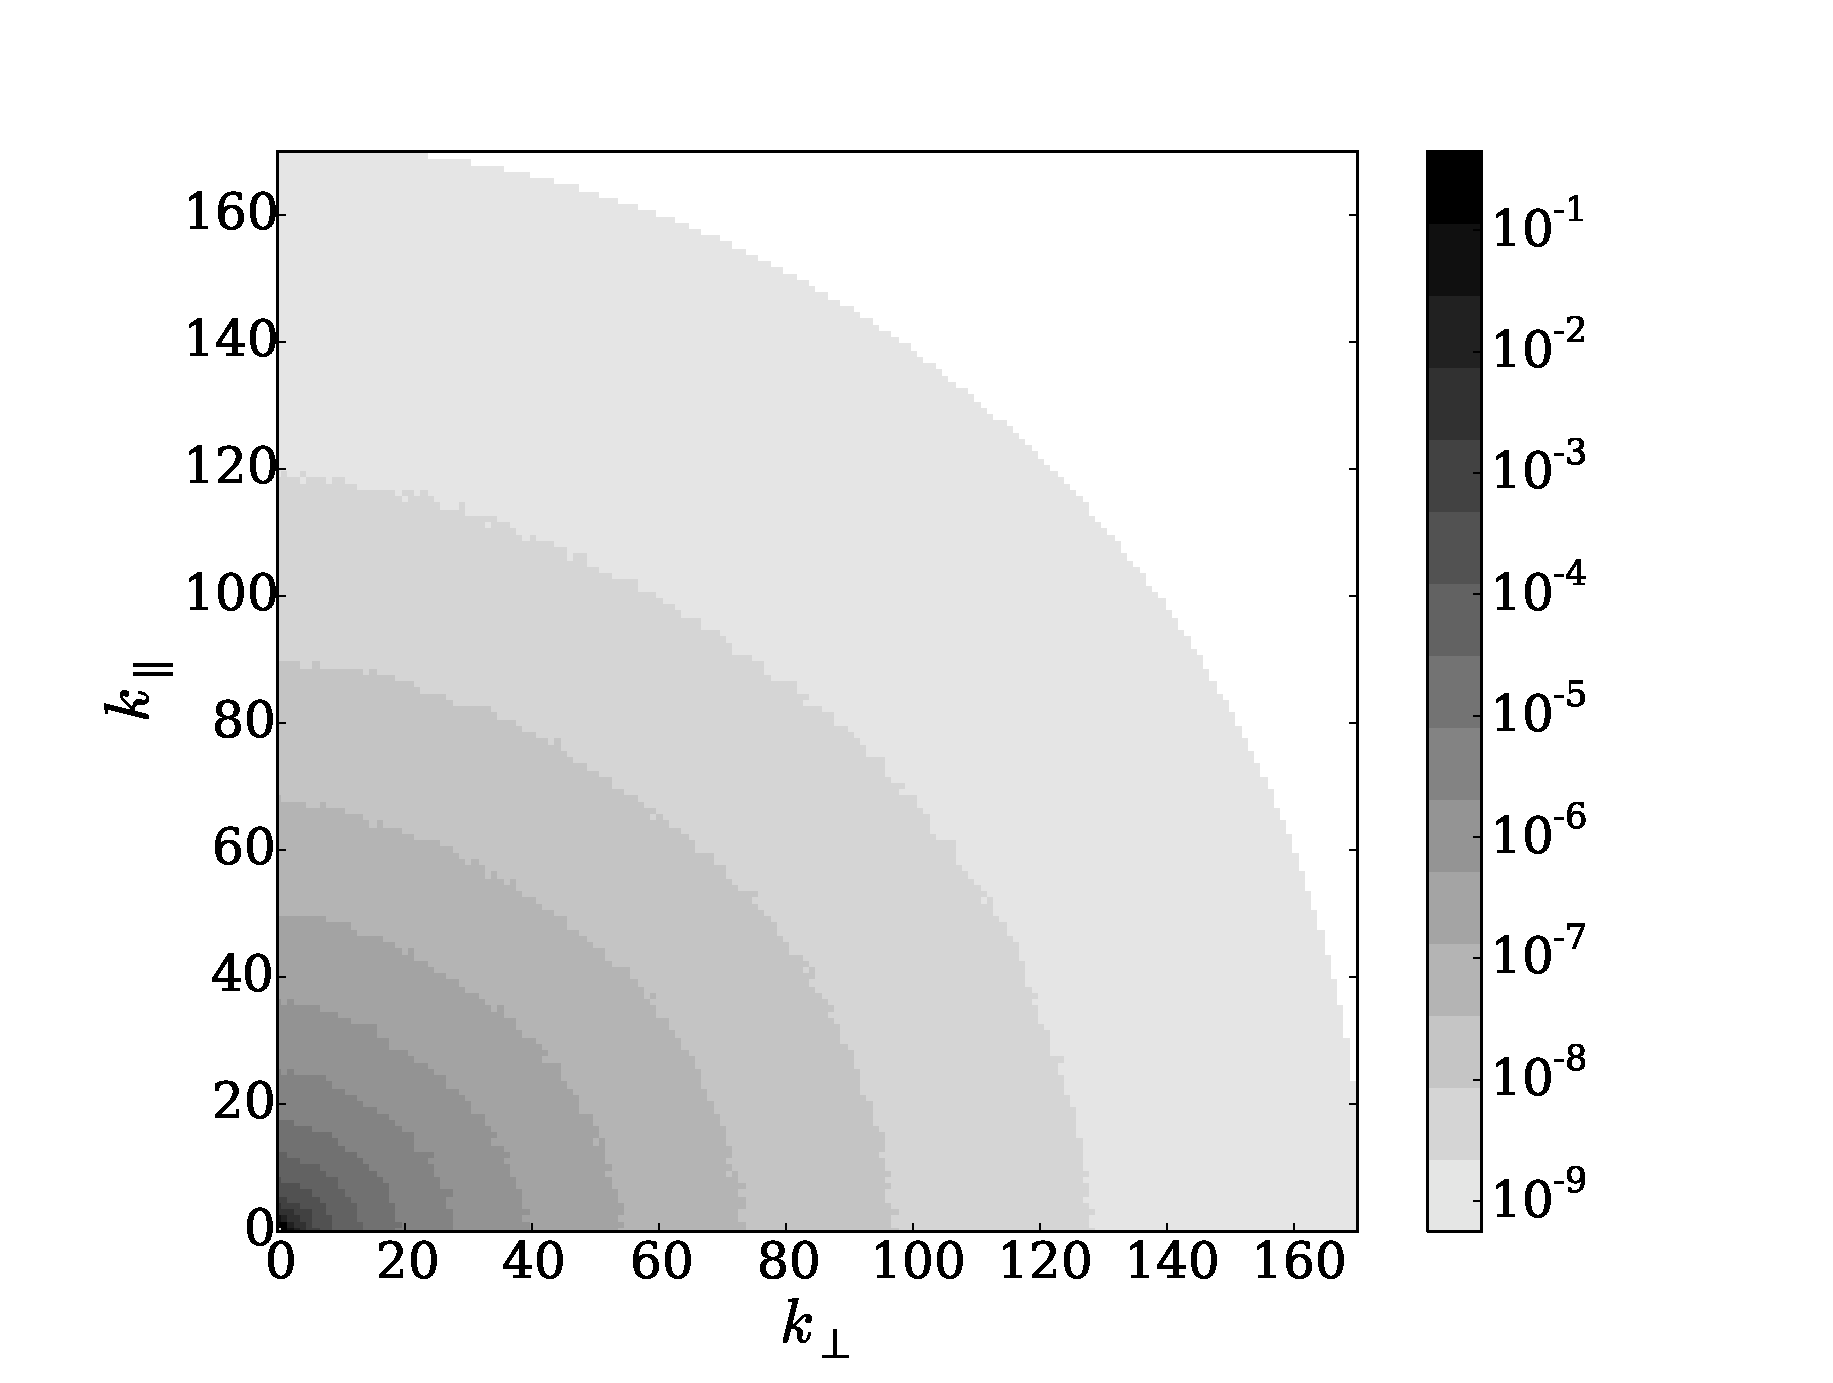
\includegraphics[width=0.7\columnwidth]{P1/fig2_B0.eps}
  \end{center}
}
\note[itemize]{
\item El espectro axisimétrico de energía $e(|\vec{k_\perp}| =
  \sqrt{k_y^2+k_z^2}, k_\parallel = k_x, t)$.
\item Para $B_0 = 0$, los contornos son círculos, como se esperaba.
}



\frame{\frametitle{Espectros de energía y escalas de tiempo dominantes}
  \underline{Isocontornos del espectro axisimétrico de energía}
  { : $B_0 = 1$}\\
  \begin{center}
    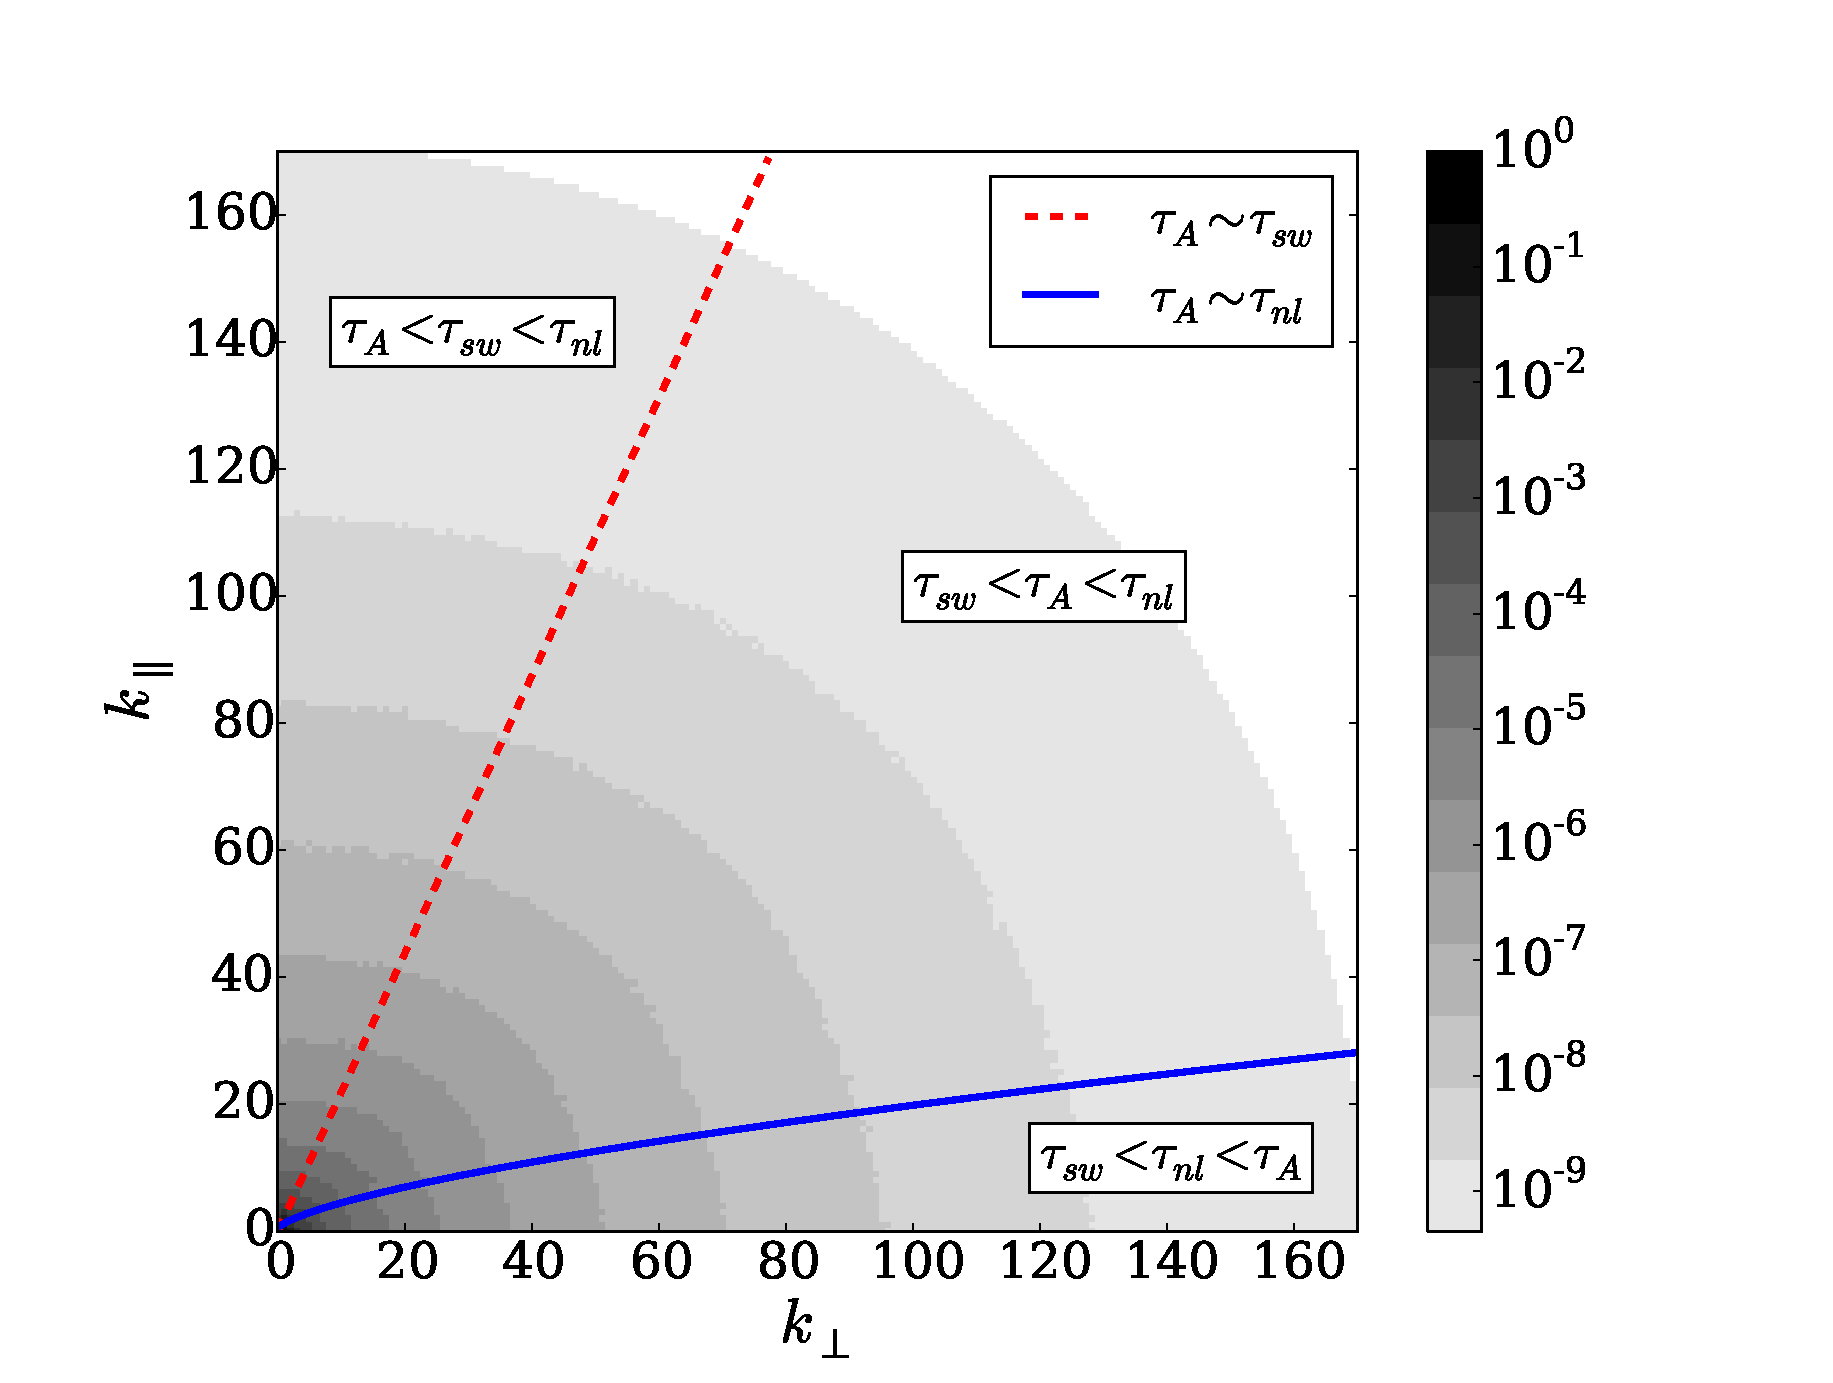
\includegraphics[width=0.7\columnwidth]{P1/fig2_B1_explanation.eps}
  \end{center}
}
\note[itemize]{
\item Aumenta $B_0$, mayor E concentrada cerca de $k_\parallel=0$
\item Formación de estructuras elongadas en la dirección del campo guía
\item
\item o, en otras palabras, del
  relativo decrecimiento de los gradientes paralelos del campo con
  respecto a los gradientes perpendiculares).
\item
\item La región con $\tau_{nl} \leq \tau_{sw}$ es un círculo pequeño
  alrededor del origen.
}




\frame{\frametitle{Espectros de energía y escalas de tiempo dominantes}
  {\underline{Isocontornos del espectro axisimétrico de energía}}\\ \vspace{1cm}
  \begin{columns}
    \column{0.5\textwidth}
    \begin{minipage}[t]{1\textwidth}
      \begin{center} 
        {$B_0 = 0.25$}\\
        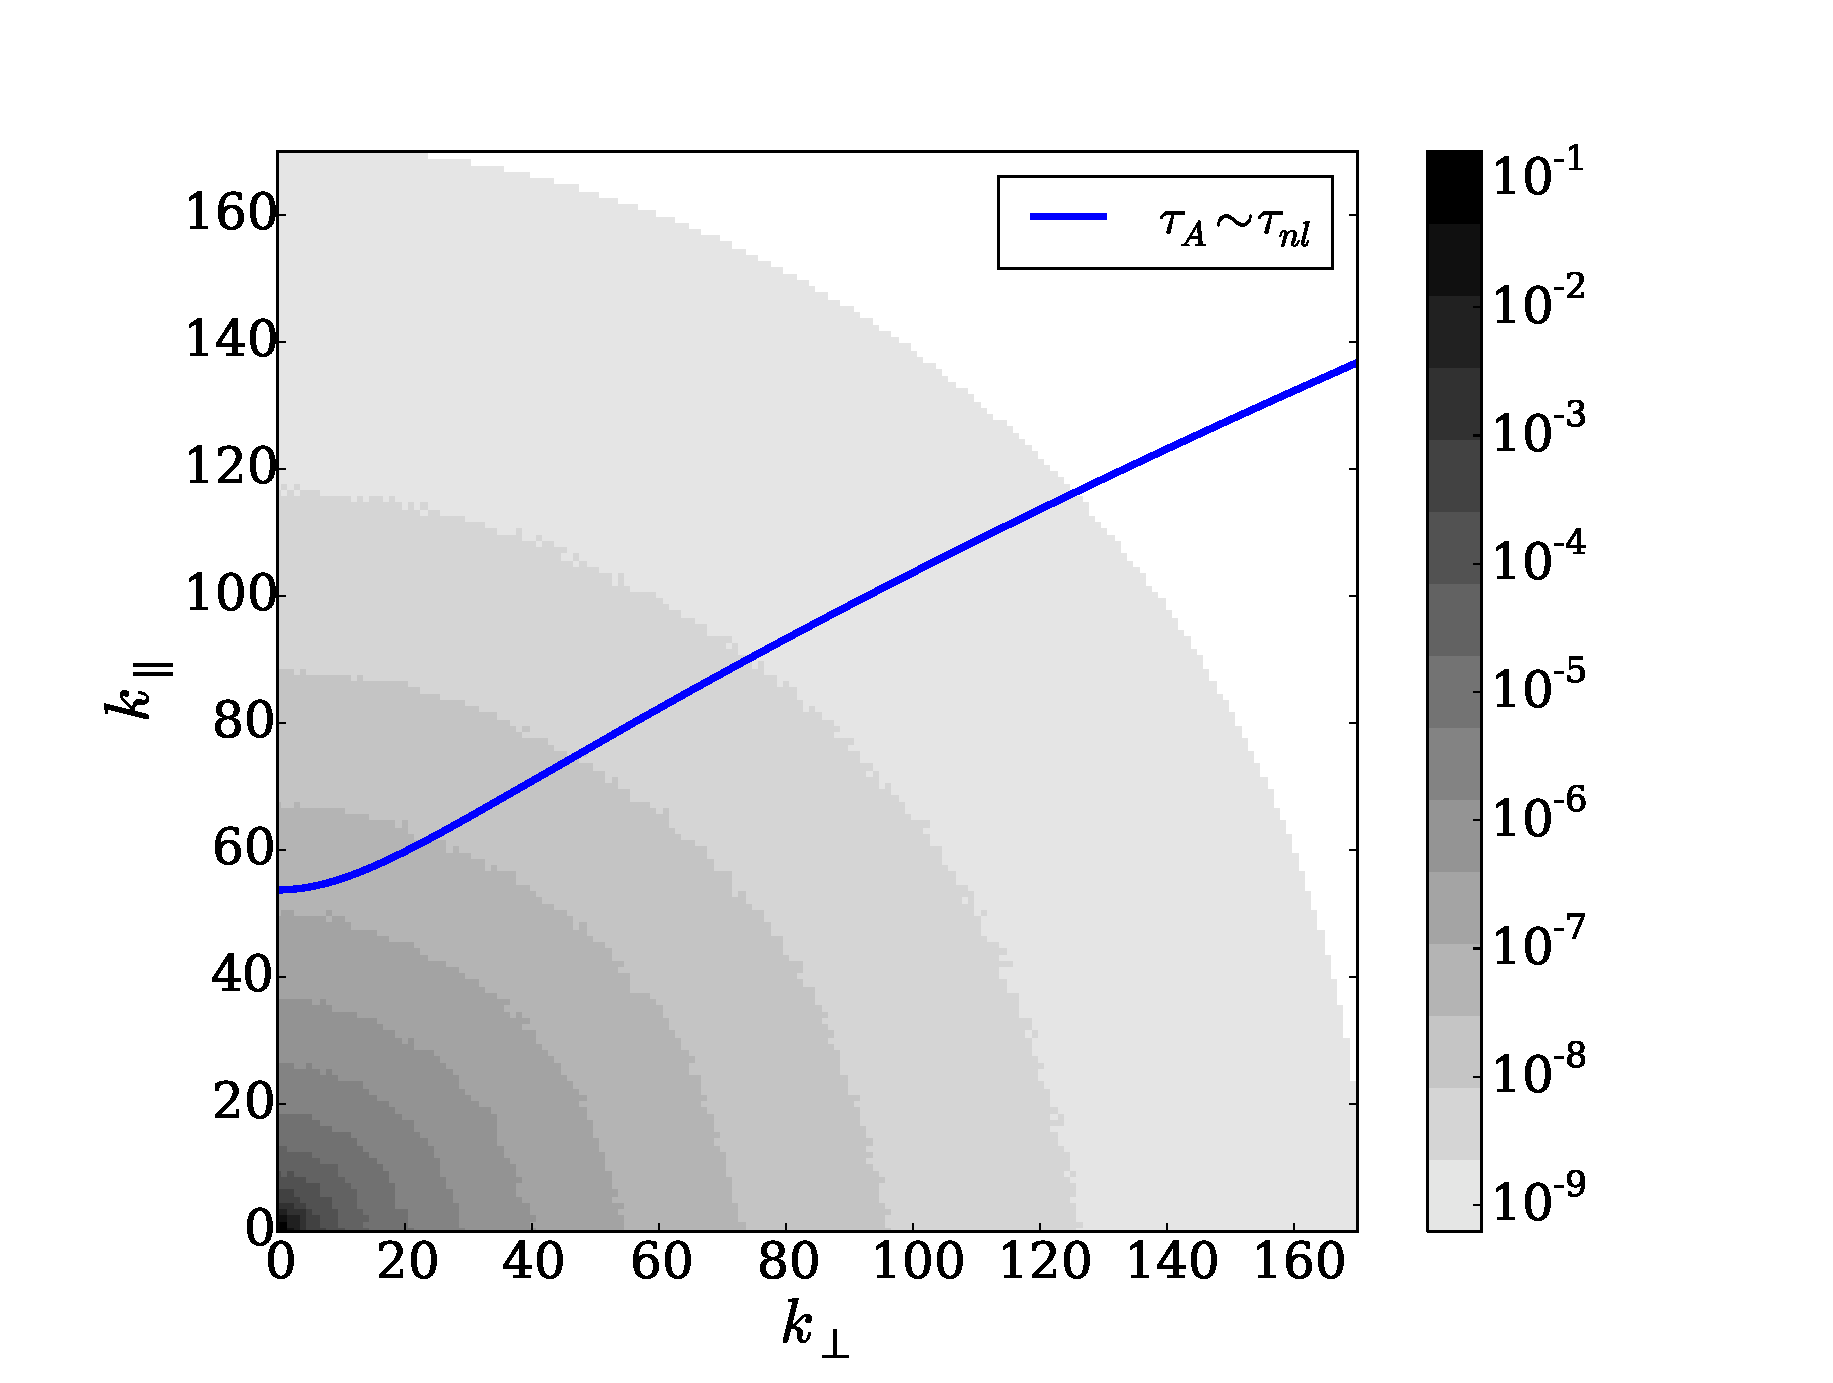
\includegraphics[width=\columnwidth]{P1/fig2_B025.eps}
      \end{center}
    \end{minipage}
    \column{0.5\textwidth}
    \begin{minipage}[t]{1\textwidth}
      \begin{center}
        {$B_0 = 8$}\\
        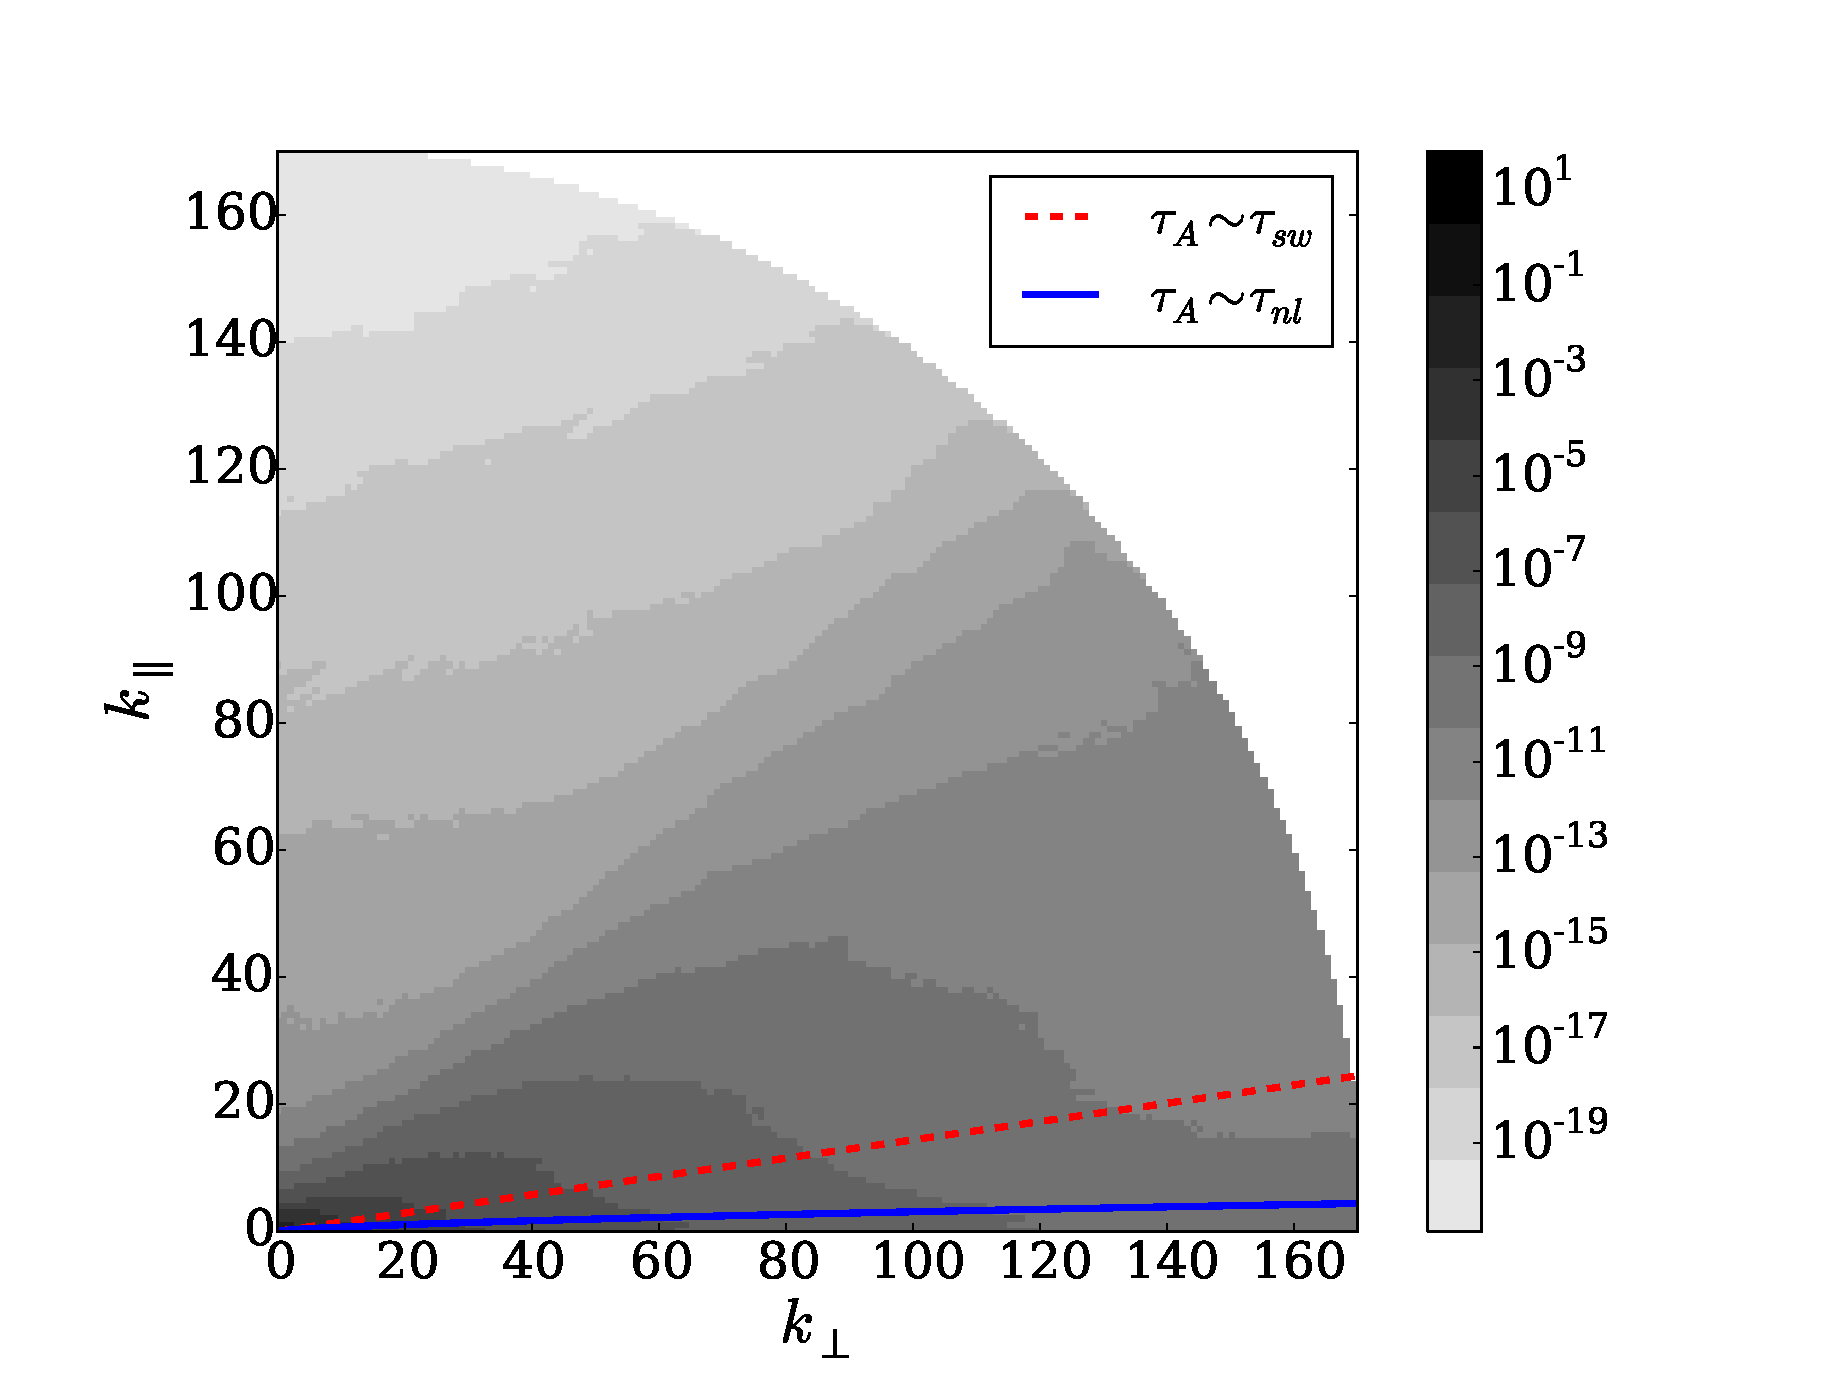
\includegraphics[width=\columnwidth]{P1/fig2_B8.eps}
      \end{center}
    \end{minipage}
  \end{columns}
}
\note[itemize]{
\item Para $B_0 = 0.25$, el tiempo de \emph{sweeping} es el más rápido
  en todos los casos..
\item Para $B_0 = 8$, mayoría de modos con tiempo de Alfvén como el
  más rápido, pero mucha energía fuera de estos modos.
}



%\subsection{Spatio-temporal spectra}
\frame{\frametitle{Espectros espacio-temporales}
  {\underline{Espectro energético normalizado $E({\bf k}, \omega)/E({\bf k})$}}
  \pause
  { : $B_0=0.25$}
  \begin{center}
    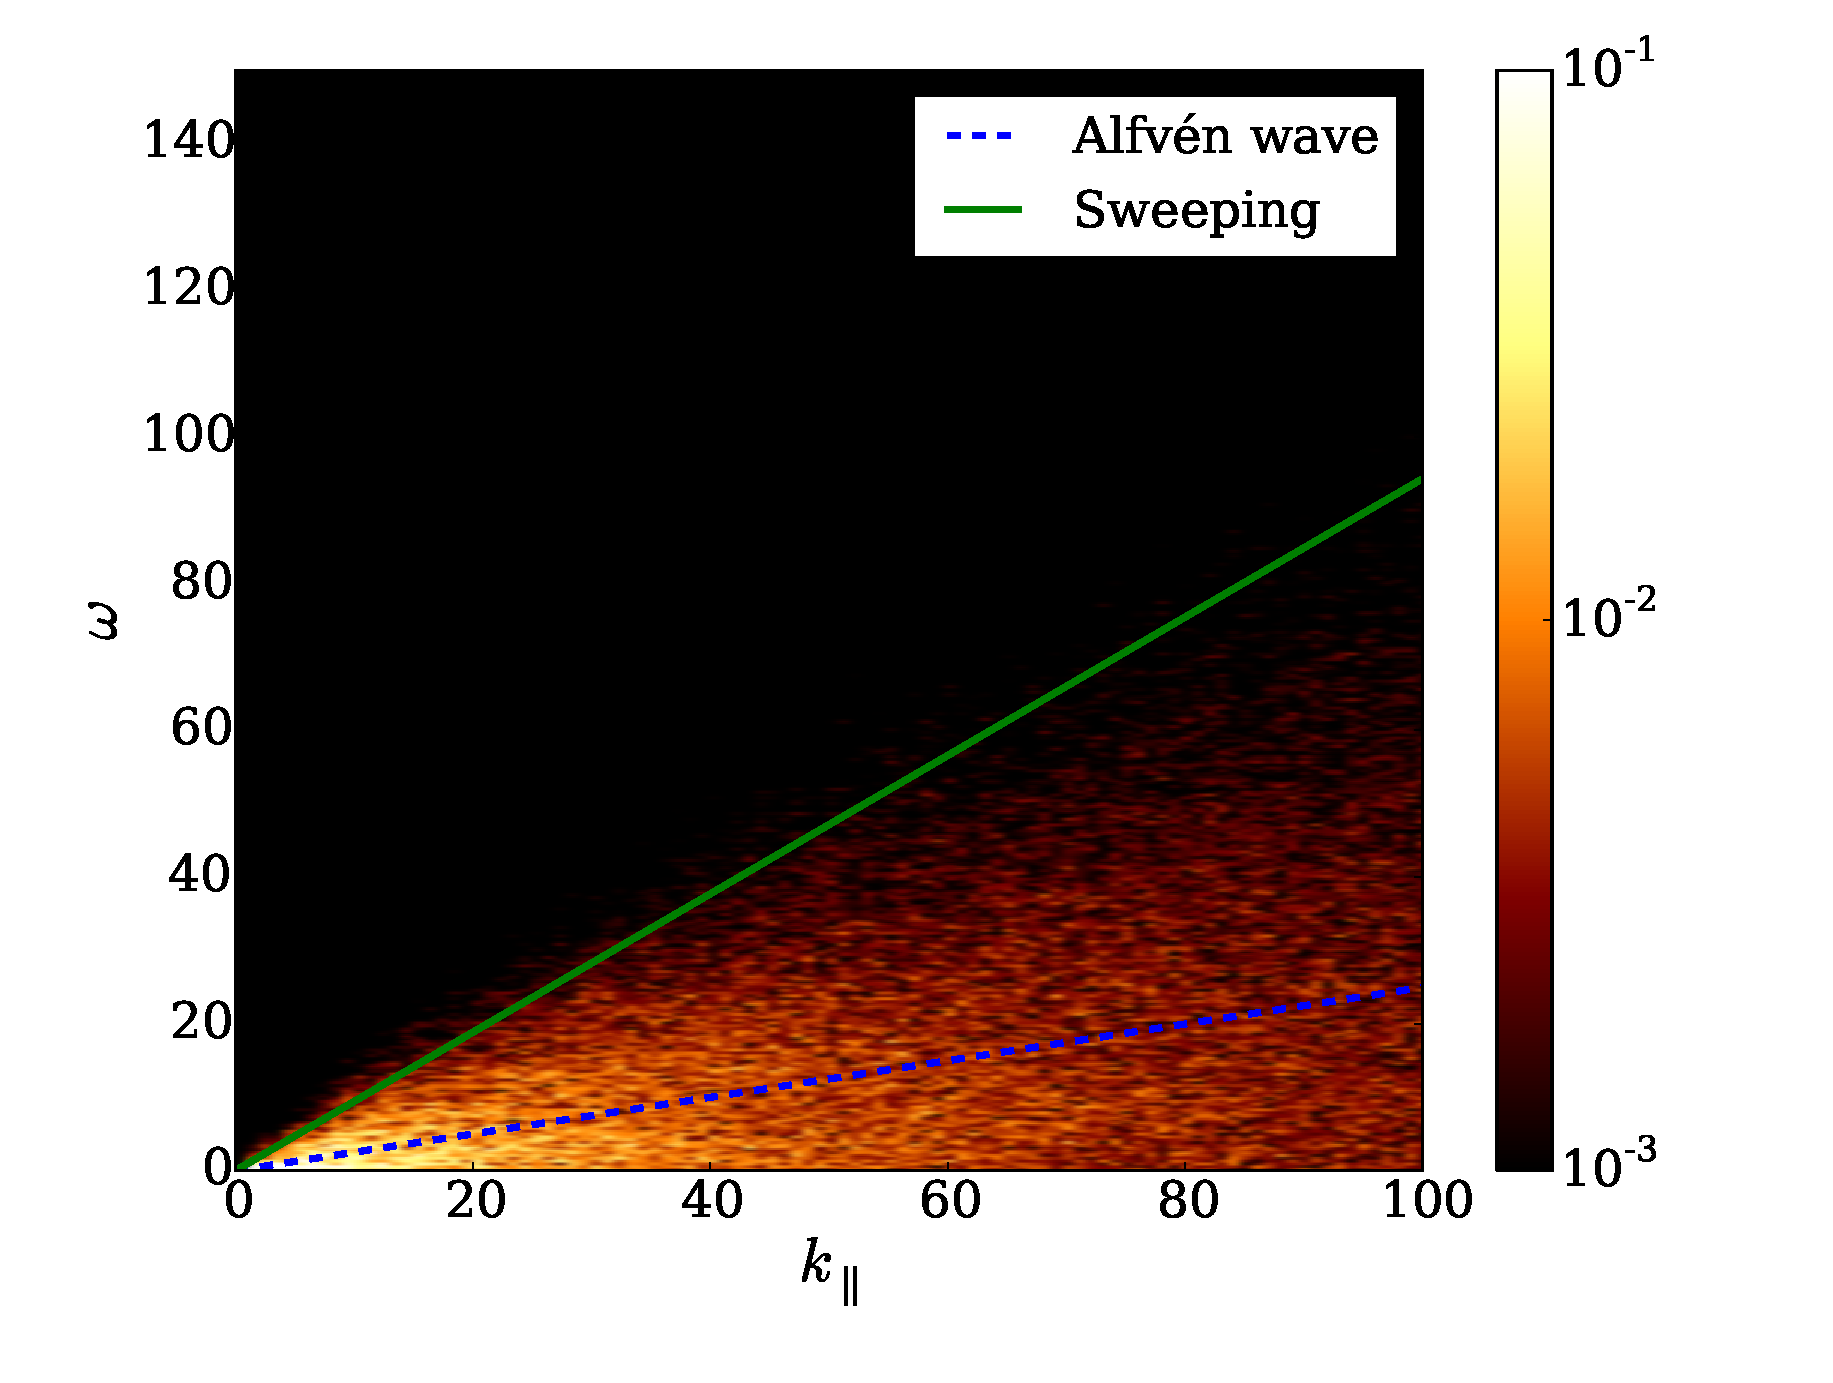
\includegraphics[width=0.7\columnwidth]{P1/fig3_B025_Etot.eps}
  \end{center}
}
\note[itemize]{
\item $k_\perp=0$ fijo. Líneas de \emph{sweeping} y Alfvén.
\item Regiones claras: mayor densidad energética.
\item Espectro: Fourier en $t$ y $r$ de $\vec{z}^\pm$. Acumulación de
  energía: dominio de un efecto físico (i.e., de su frecuencia
  asociada) en la dinámica del plasma a una dada escala $\sim
  1/k_\parallel$.
\item Para $B_0 = 0.25$, dispersión de energía por debajo de la línea
  de \emph{sweeping}. Excitación en modos con frecuencias iguales o
  menores que $\omega = v_{rms} k_\parallel$, indicando que las
  estructuras de escalas pequeñas están siendo advectadas por todas
  las velocidades iguales o menores a $v_{rms}$ $\Rightarrow$ embudo.
\item Pequeña acumulación cerca de la dispersión de Alfvén para
  $k_\parallel$ pequeños.
}



\frame{\frametitle{Espectros espacio-temporales}
  {\underline{Espectro energético normalizado $E({\bf k}, \omega)/E({\bf k})$} : $B_0=1$}
  \begin{center}
    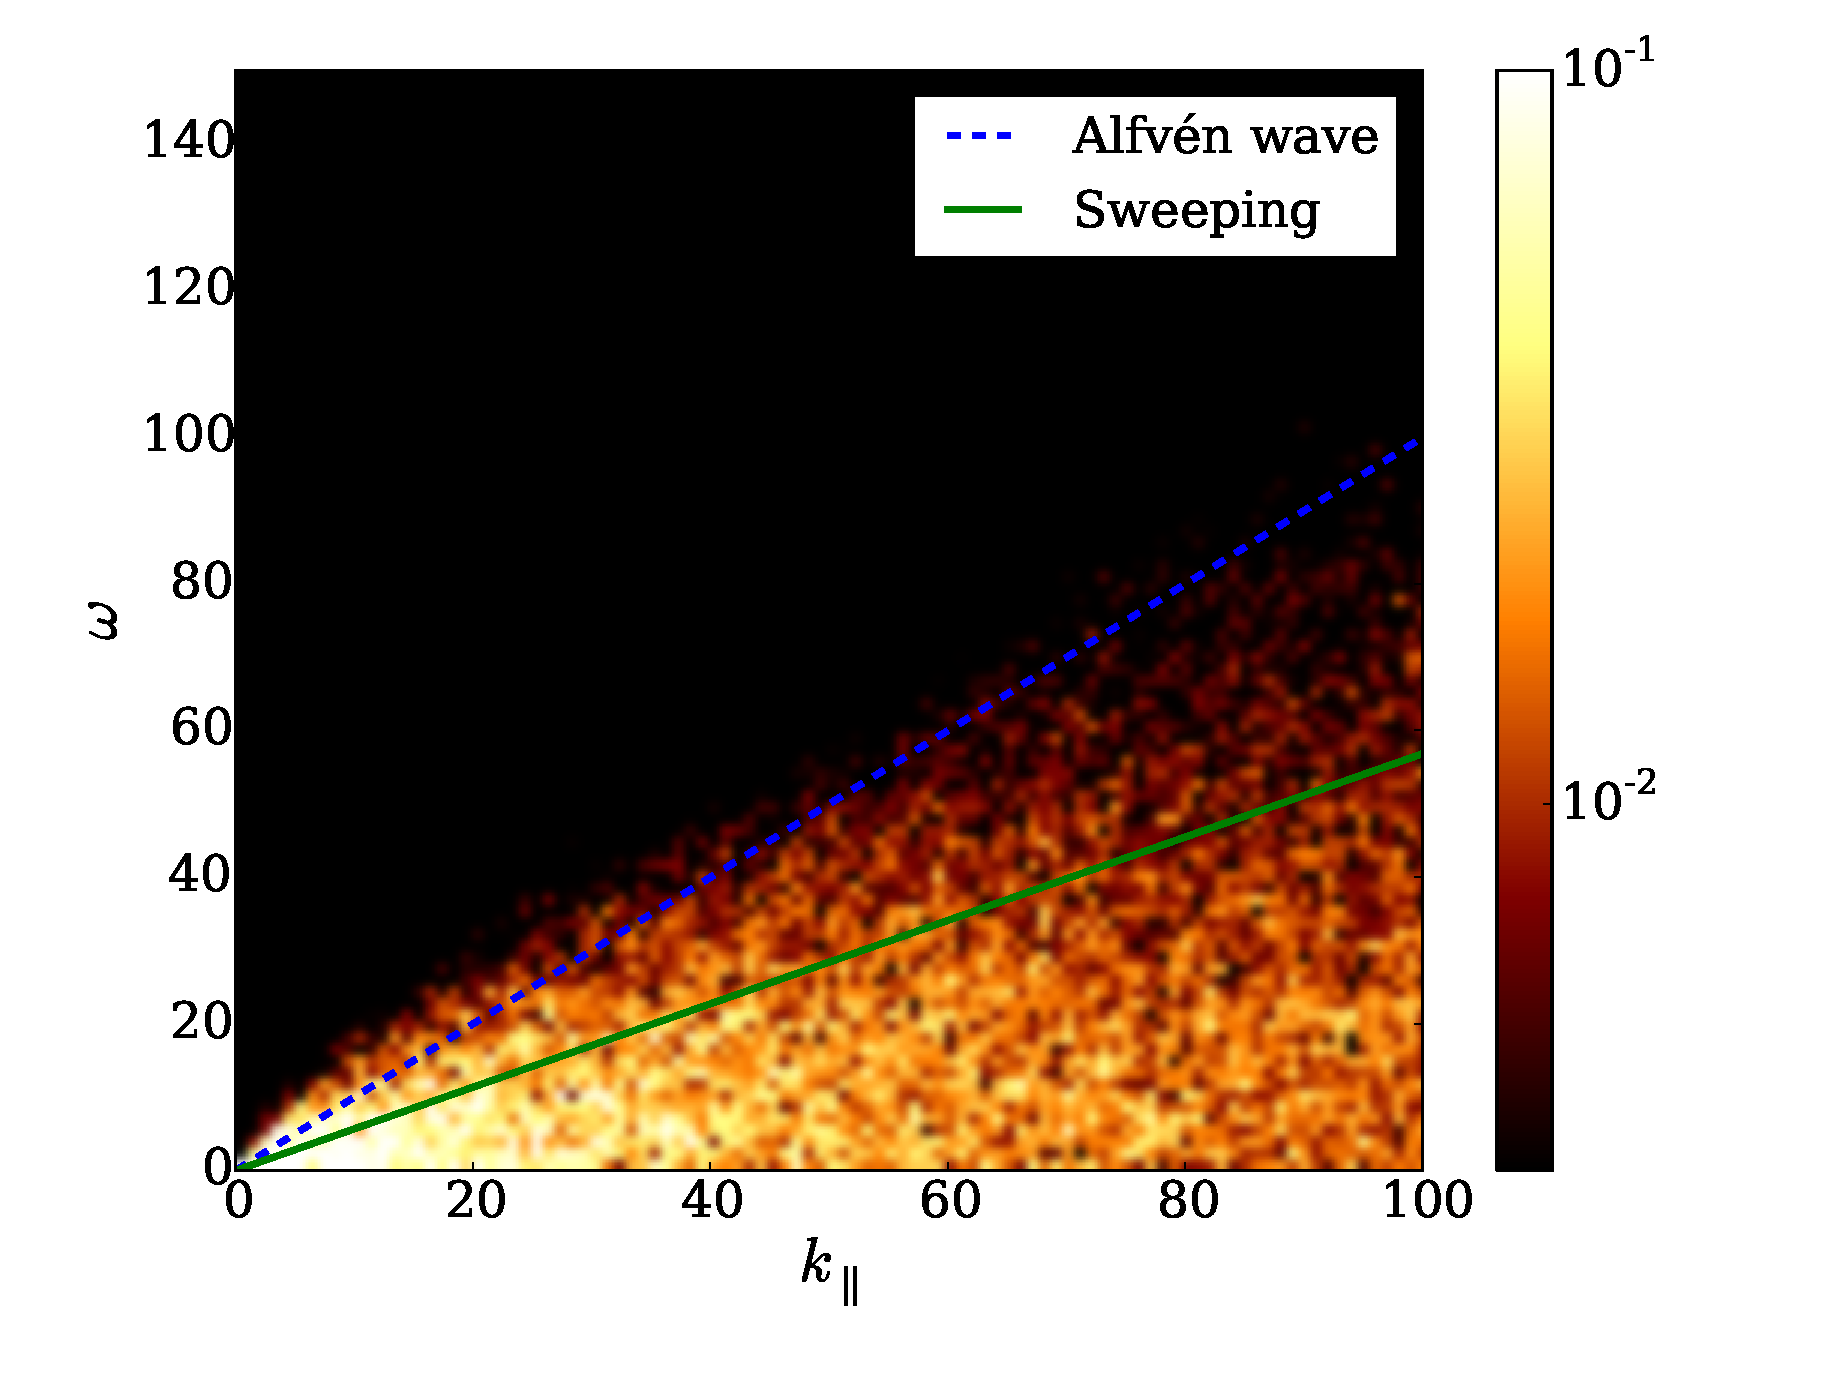
\includegraphics[width=0.7\columnwidth]{P1/fig3_B1_Etot.eps}
  \end{center}
}
\note[itemize]{
\item $B_0=1$, parte de E por encima de \textit{sweeping}, y siguiendo la relación de
  dispersión de Alfvén.
\item Igualmente, espectro amplio, con mucha energía en embudo.
}



\frame{\frametitle{Espectros espacio-temporales}
  {\underline{Espectro energético normalizado $E({\bf k}, \omega)/E({\bf k})$} : $B_0=8$}
  \begin{center}
    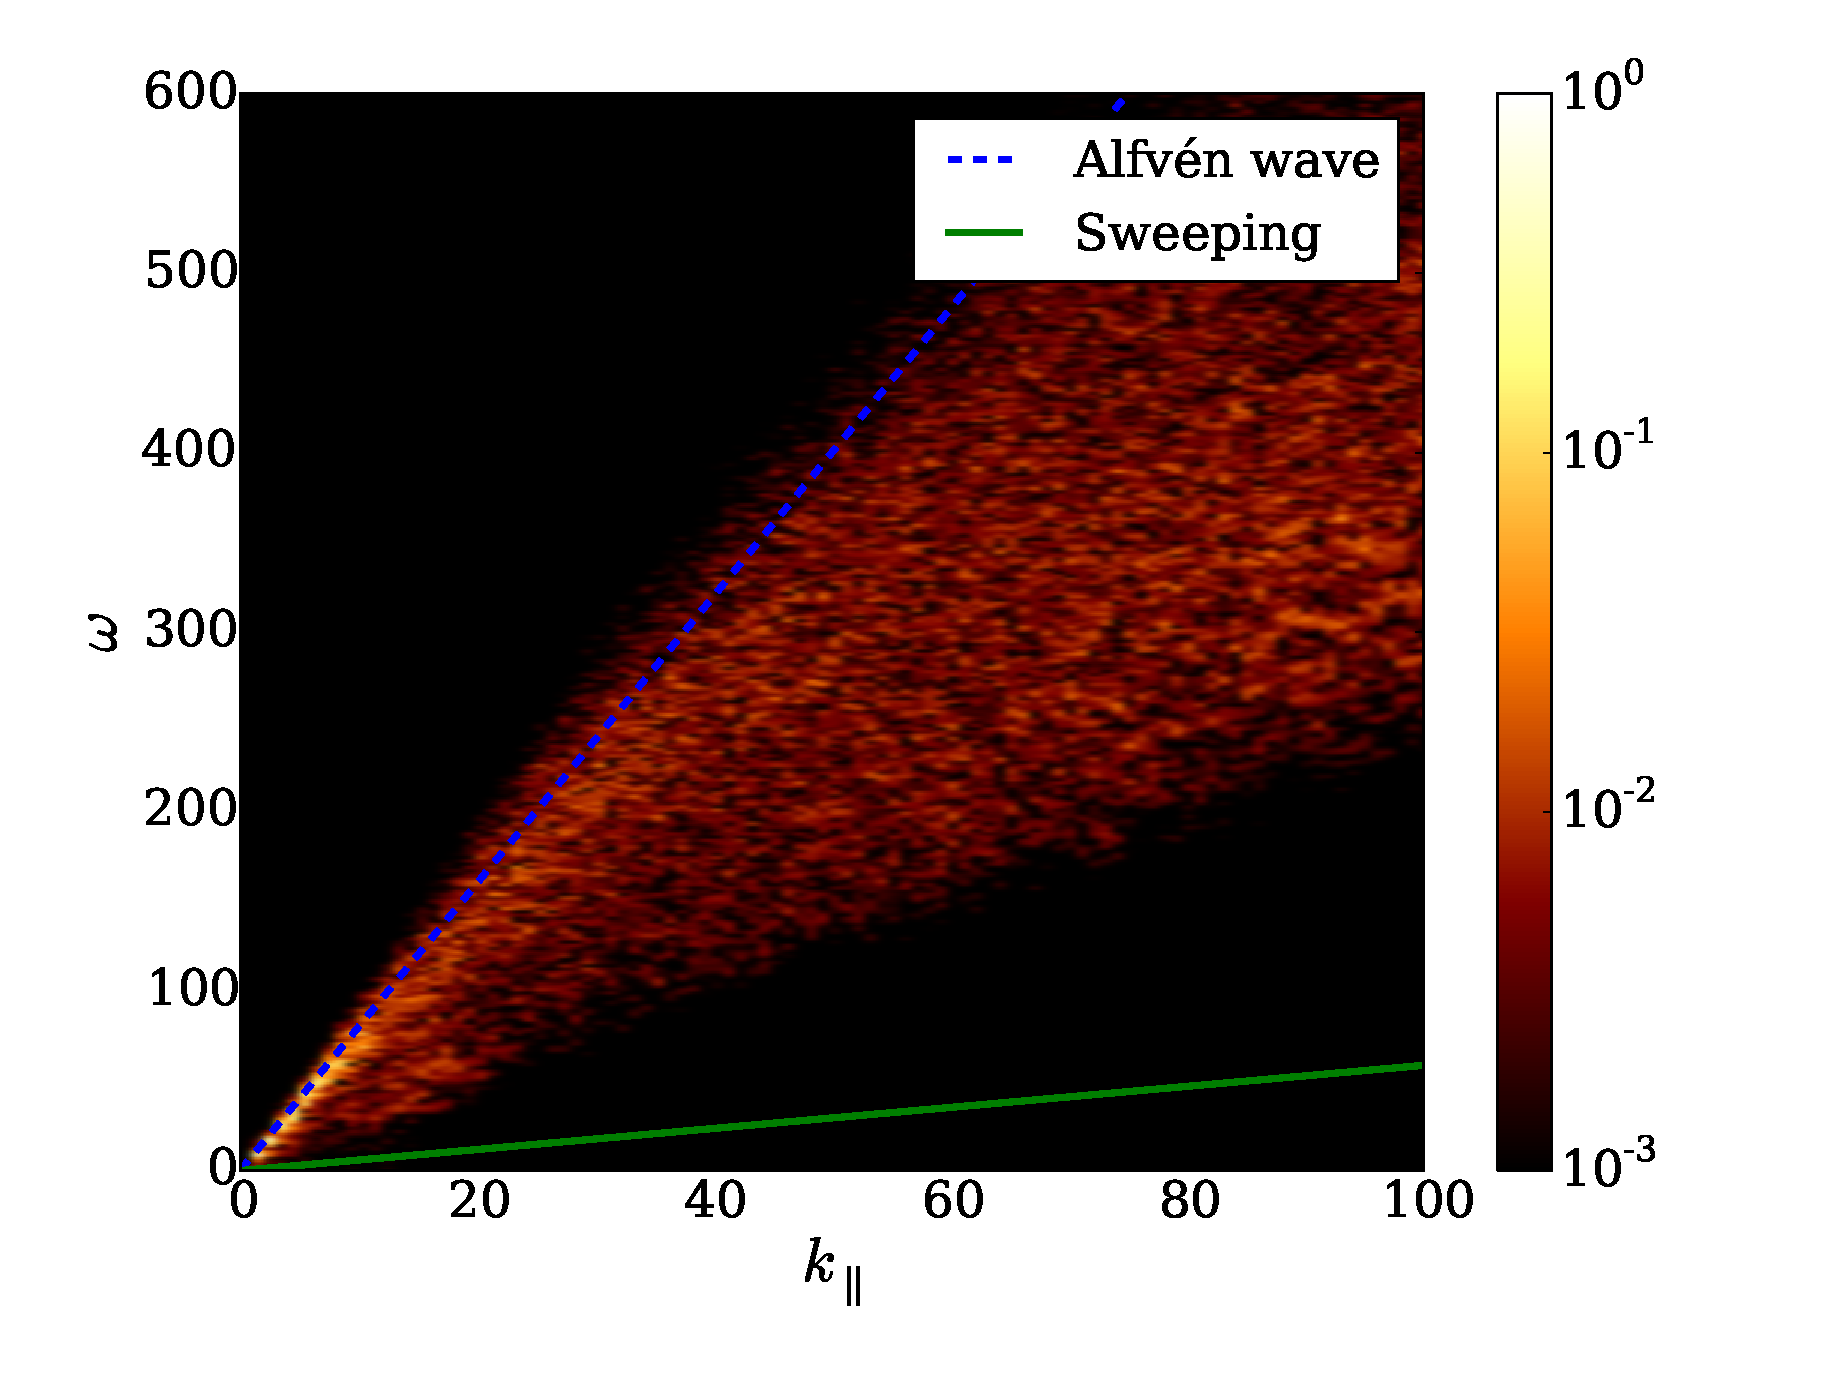
\includegraphics[width=0.7\columnwidth]{P1/fig3_B8_Etot.eps}
  \end{center}
}
\note[itemize]{
\item $B_0=8$, E alrededor de Alfvén, ppalmente hasta $k_\parallel \approx 10$.
\item Luego, se dispersa hacia \textit{sweeping}.
\item Este comportamiento indica una competición entre el tiempo de
  \textit{sweeping} y el tiempo de Alfvén, con este último resultando
  dominante a grandes escalas para valores de $B_0$ grandes.
\item Meyrand (2016): transición de un
  espectro ondular estrecho a un espectro más amplio, aunque la escala
  y el mecanismo responsable para esta transición no fue
  estudiado. Como confirmaremos posteriormente, la competencia entre
  los tiempos de \textit{sweeping} y de Alfvén como el tiempo de
  descorrelación dominante es la responsable del cambio observado en
  el comportamiento del espectro.
 }




%\subsection{Correlation functions and decorrelation time}
\frame{\frametitle{Funciones de correlación: $\Gamma(k_\perp,k_\parallel,\tau)$}
  \pause
  Caso con $B_0 = 1$\vspace{10pt}
  \begin{columns}
    \column{0.5\textwidth}
    \begin{minipage}[t]{1\textwidth}
      \begin{center} 
        $\Gamma(k_\perp=0,k_\parallel=k_0,\tau)$ \\
        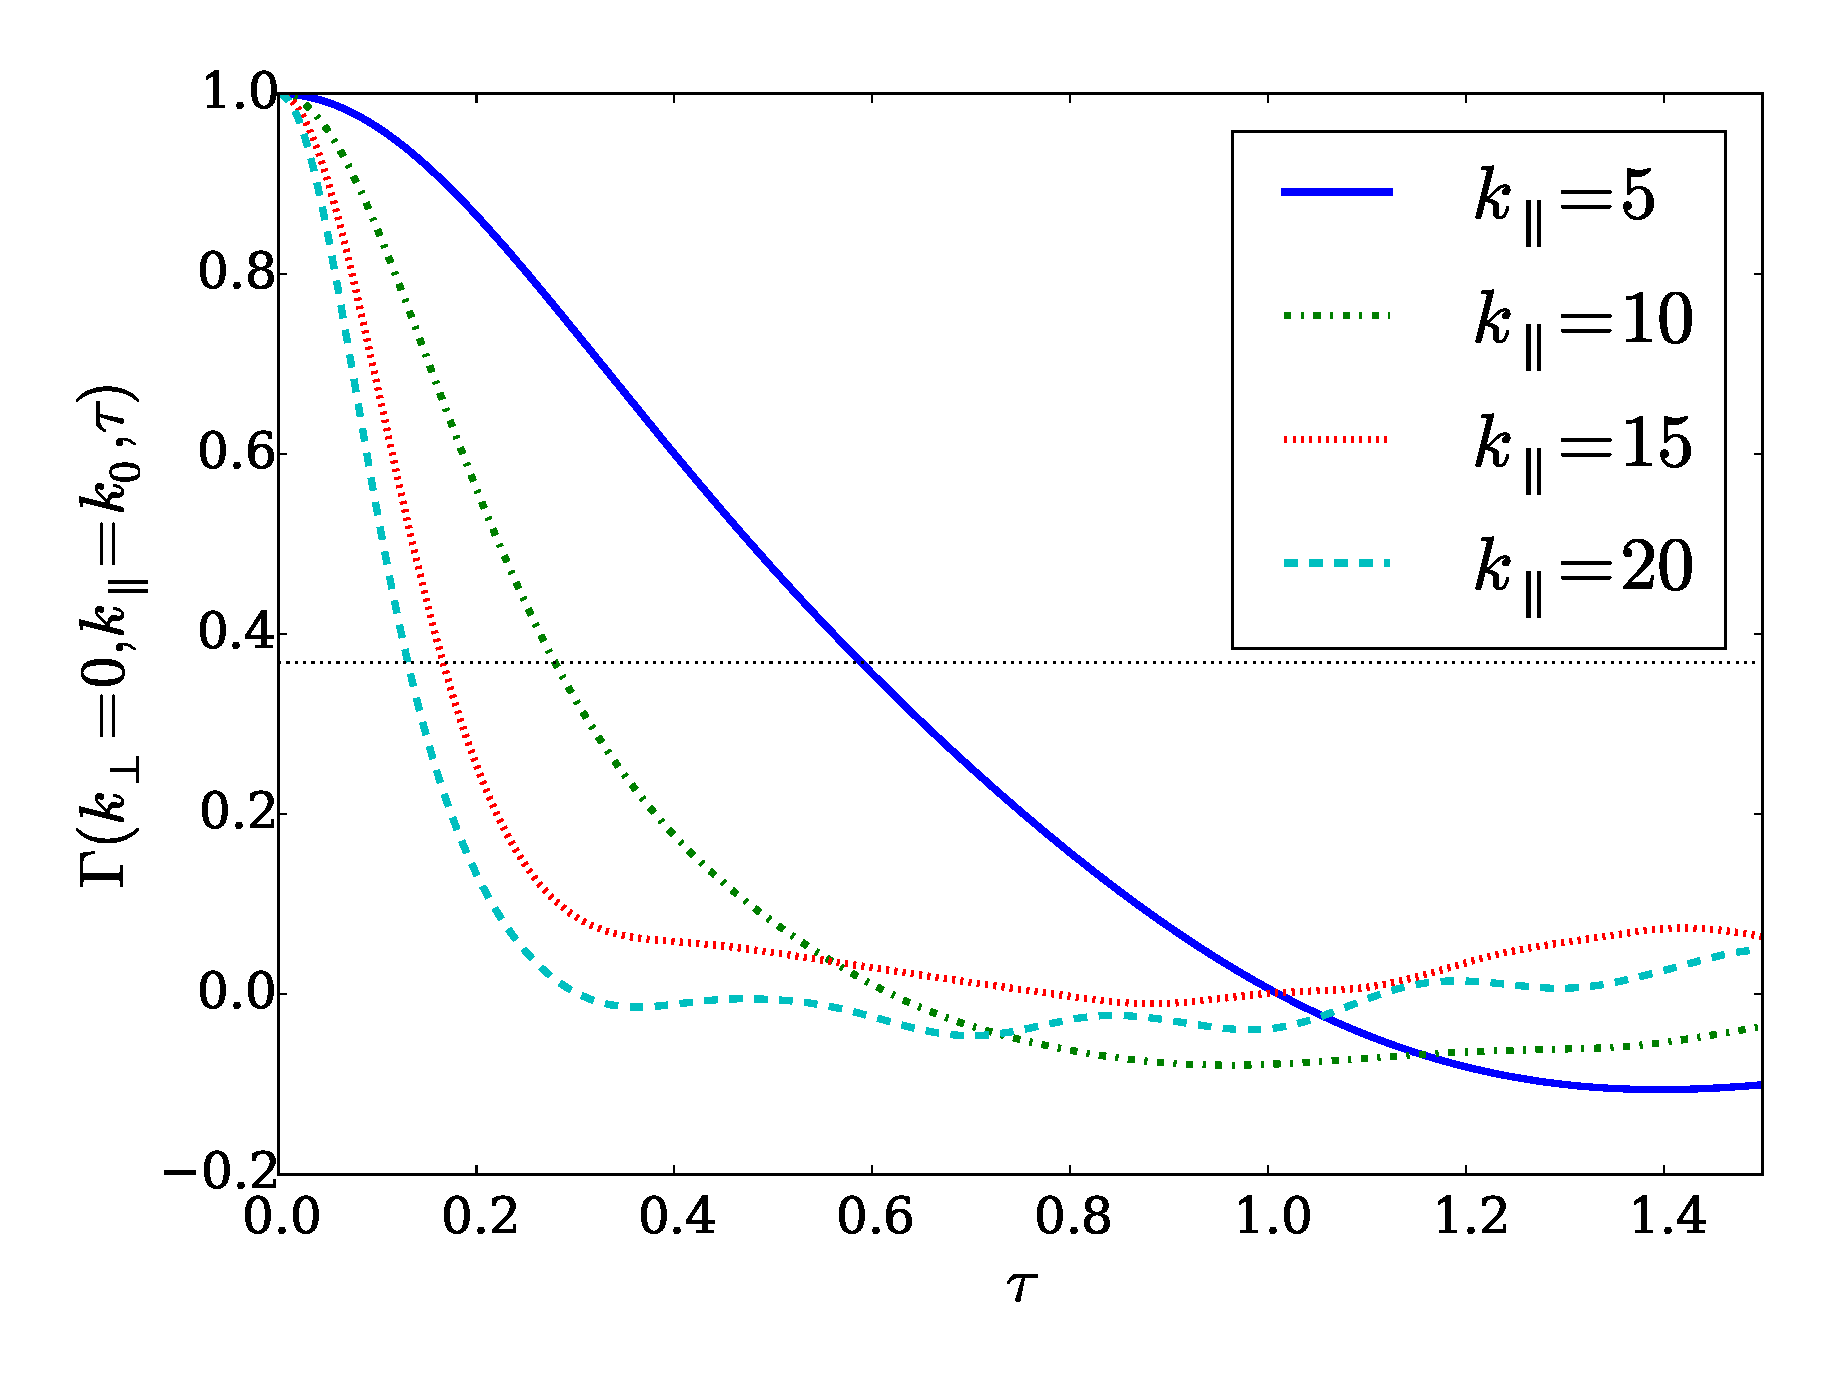
\includegraphics[width=0.9\columnwidth]{P1/fig4_B1_b_kperp.eps}
      \end{center}
    \end{minipage}
    \column{0.5\textwidth}
    \begin{minipage}[t]{1\textwidth}
      \begin{center}
        $\Gamma(k_\perp=k_0,k_\parallel=0,\tau)$ \\
        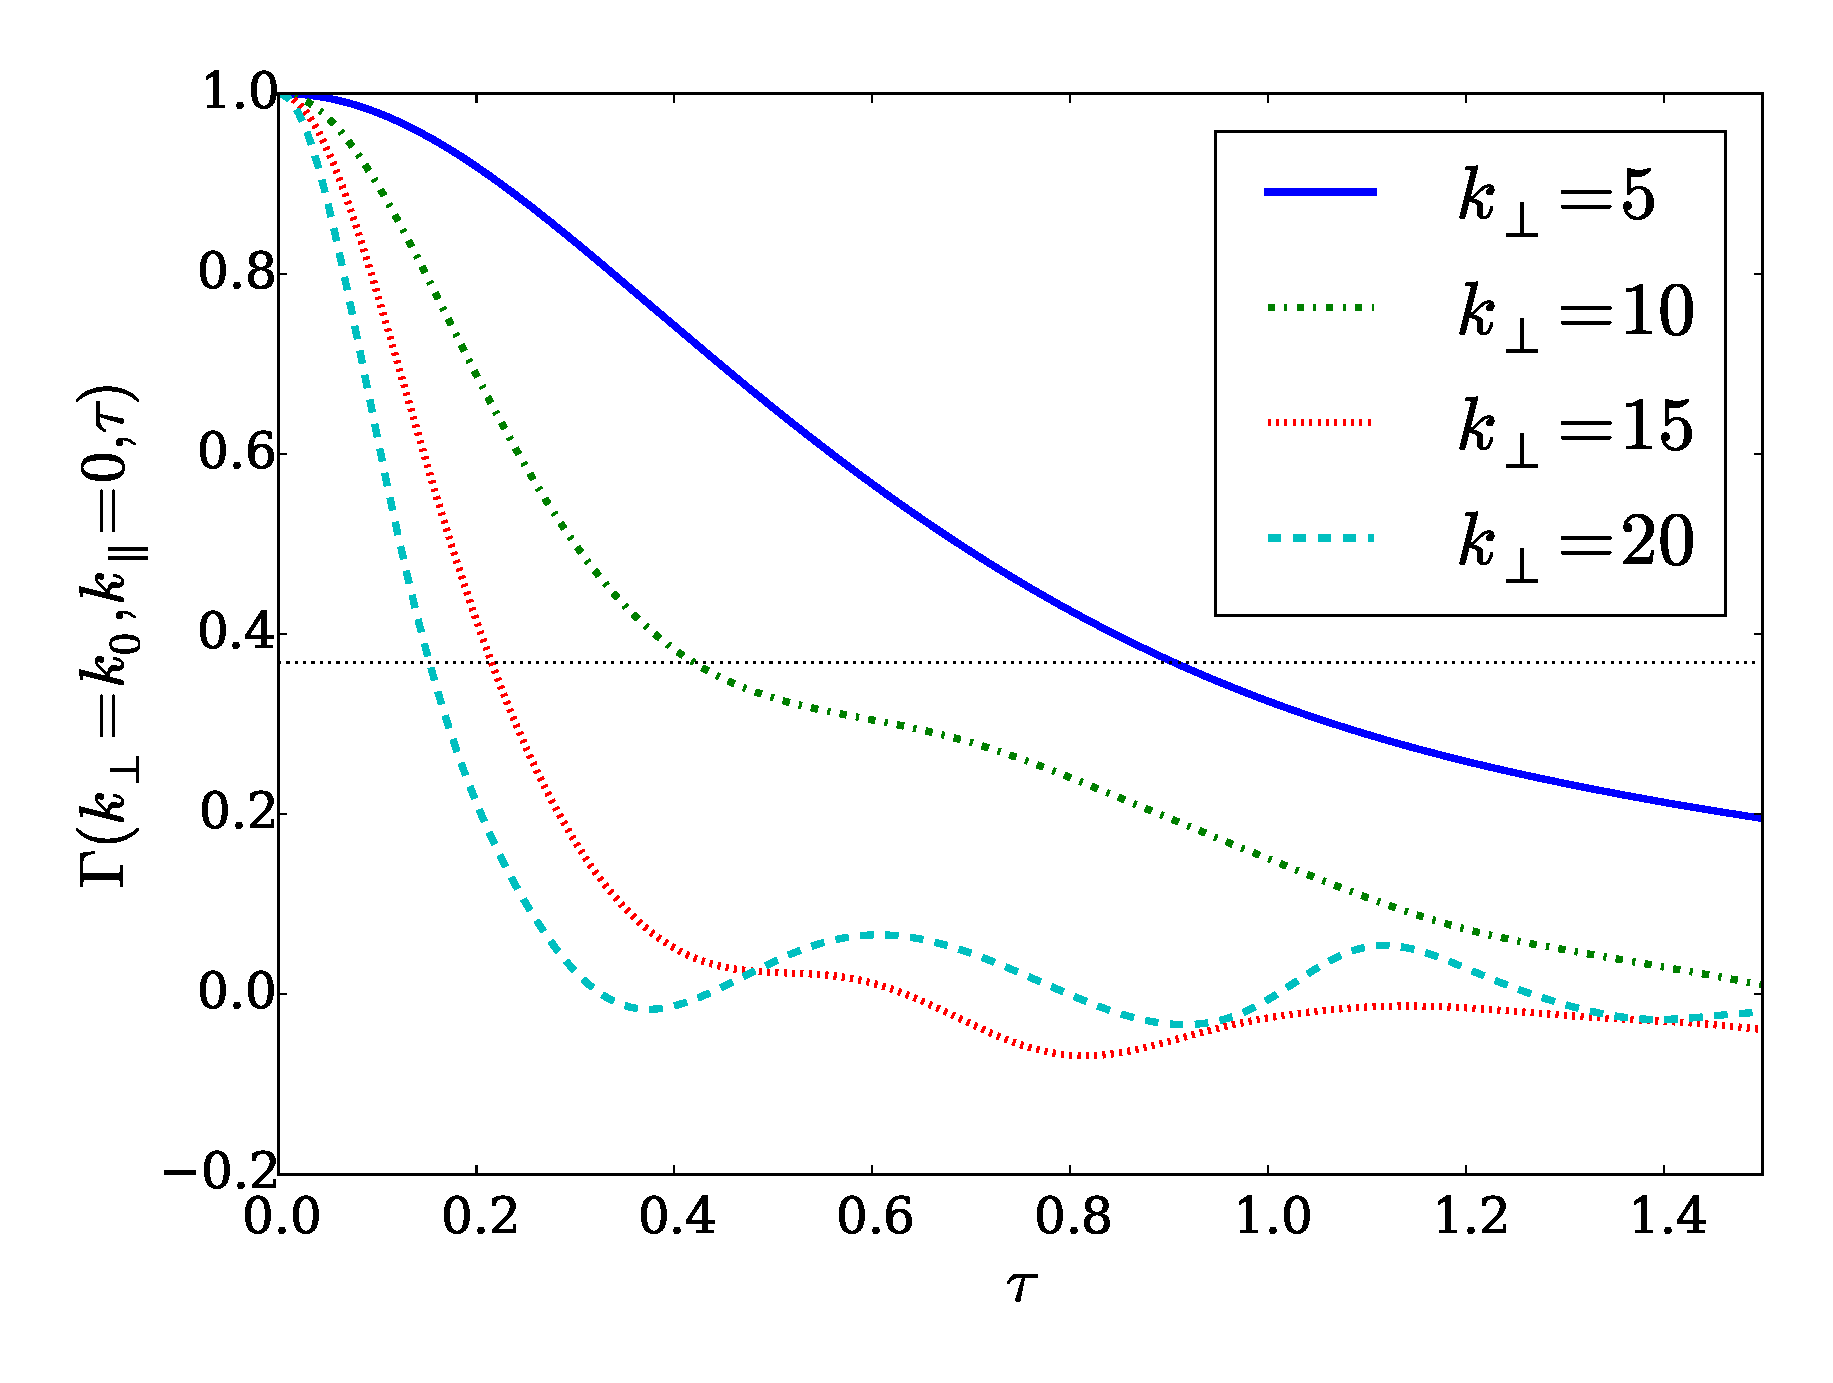
\includegraphics[width=0.9\columnwidth]{P1/fig4_B1_b_kpara.eps}
      \end{center}
    \end{minipage}
  \end{columns}
}
\note[itemize]{
\item ¿Qué tiempo controla la descorrelación temporal? Mecesitamos comparar el
  tiempo de descorrelación en las distintas escalas con el
  comportamiento teórico esperado para cada proceso físico.
\item Correlación aproximadamente decaimiento exponencial
  $\Gamma(\vec{k},\tau) \sim e^{-\tau/\tau_D(\vec{k})}$
\item El valor de $\tau$ para el cual $\Gamma=1/e$ corresponde al
  tiempo de descorrelación $\tau_D$ para cada valor de $\vec{k}$.
}

  


\frame{\frametitle{Tiempos de descorrelación}
  \pause
  {\Large \underline{Tiempo de descorrelación para el caso isotrópico $B_0=0$}}
  \begin{center}
    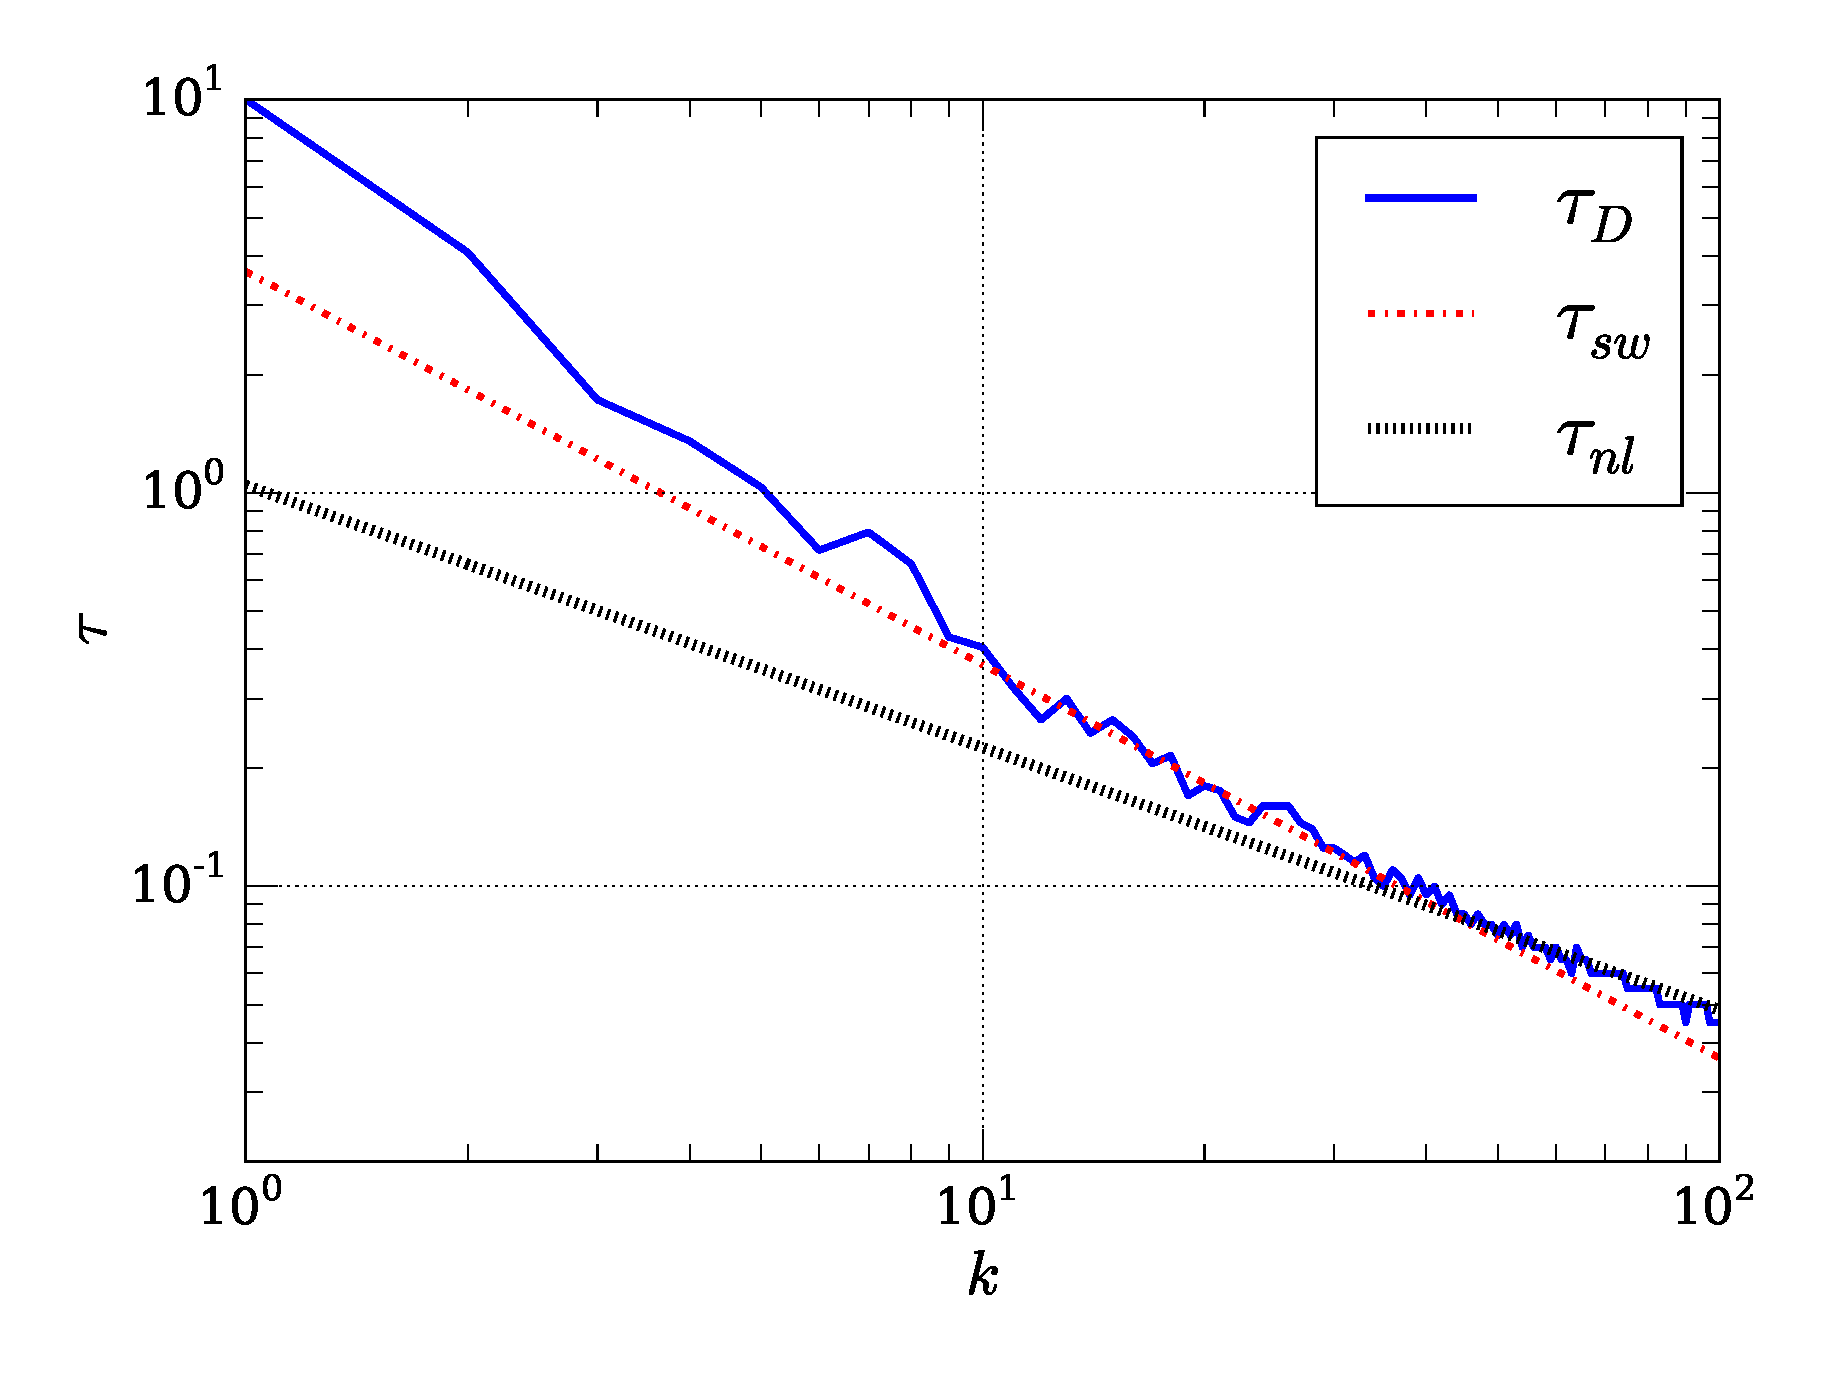
\includegraphics[width=0.7\columnwidth]{P1/fig5_B0_b.eps}
  \end{center}
}
\note[itemize]{
\item $\tau_D$ se encuentra en buen acuerdo con $\tau_{sw}$.
\item Resultados consistentes con Servidio (2011).
}


\frame{\frametitle{Tiempos de descorrelación}
  {\Large \underline{Tiempos de descorrelación: $B_0=1$ y $k_\perp = k_0$}}
  \begin{columns}
    \column{0.5\textwidth}
    \begin{minipage}[t]{1\textwidth}
      \begin{center}
        $k_\perp = 0$\\
        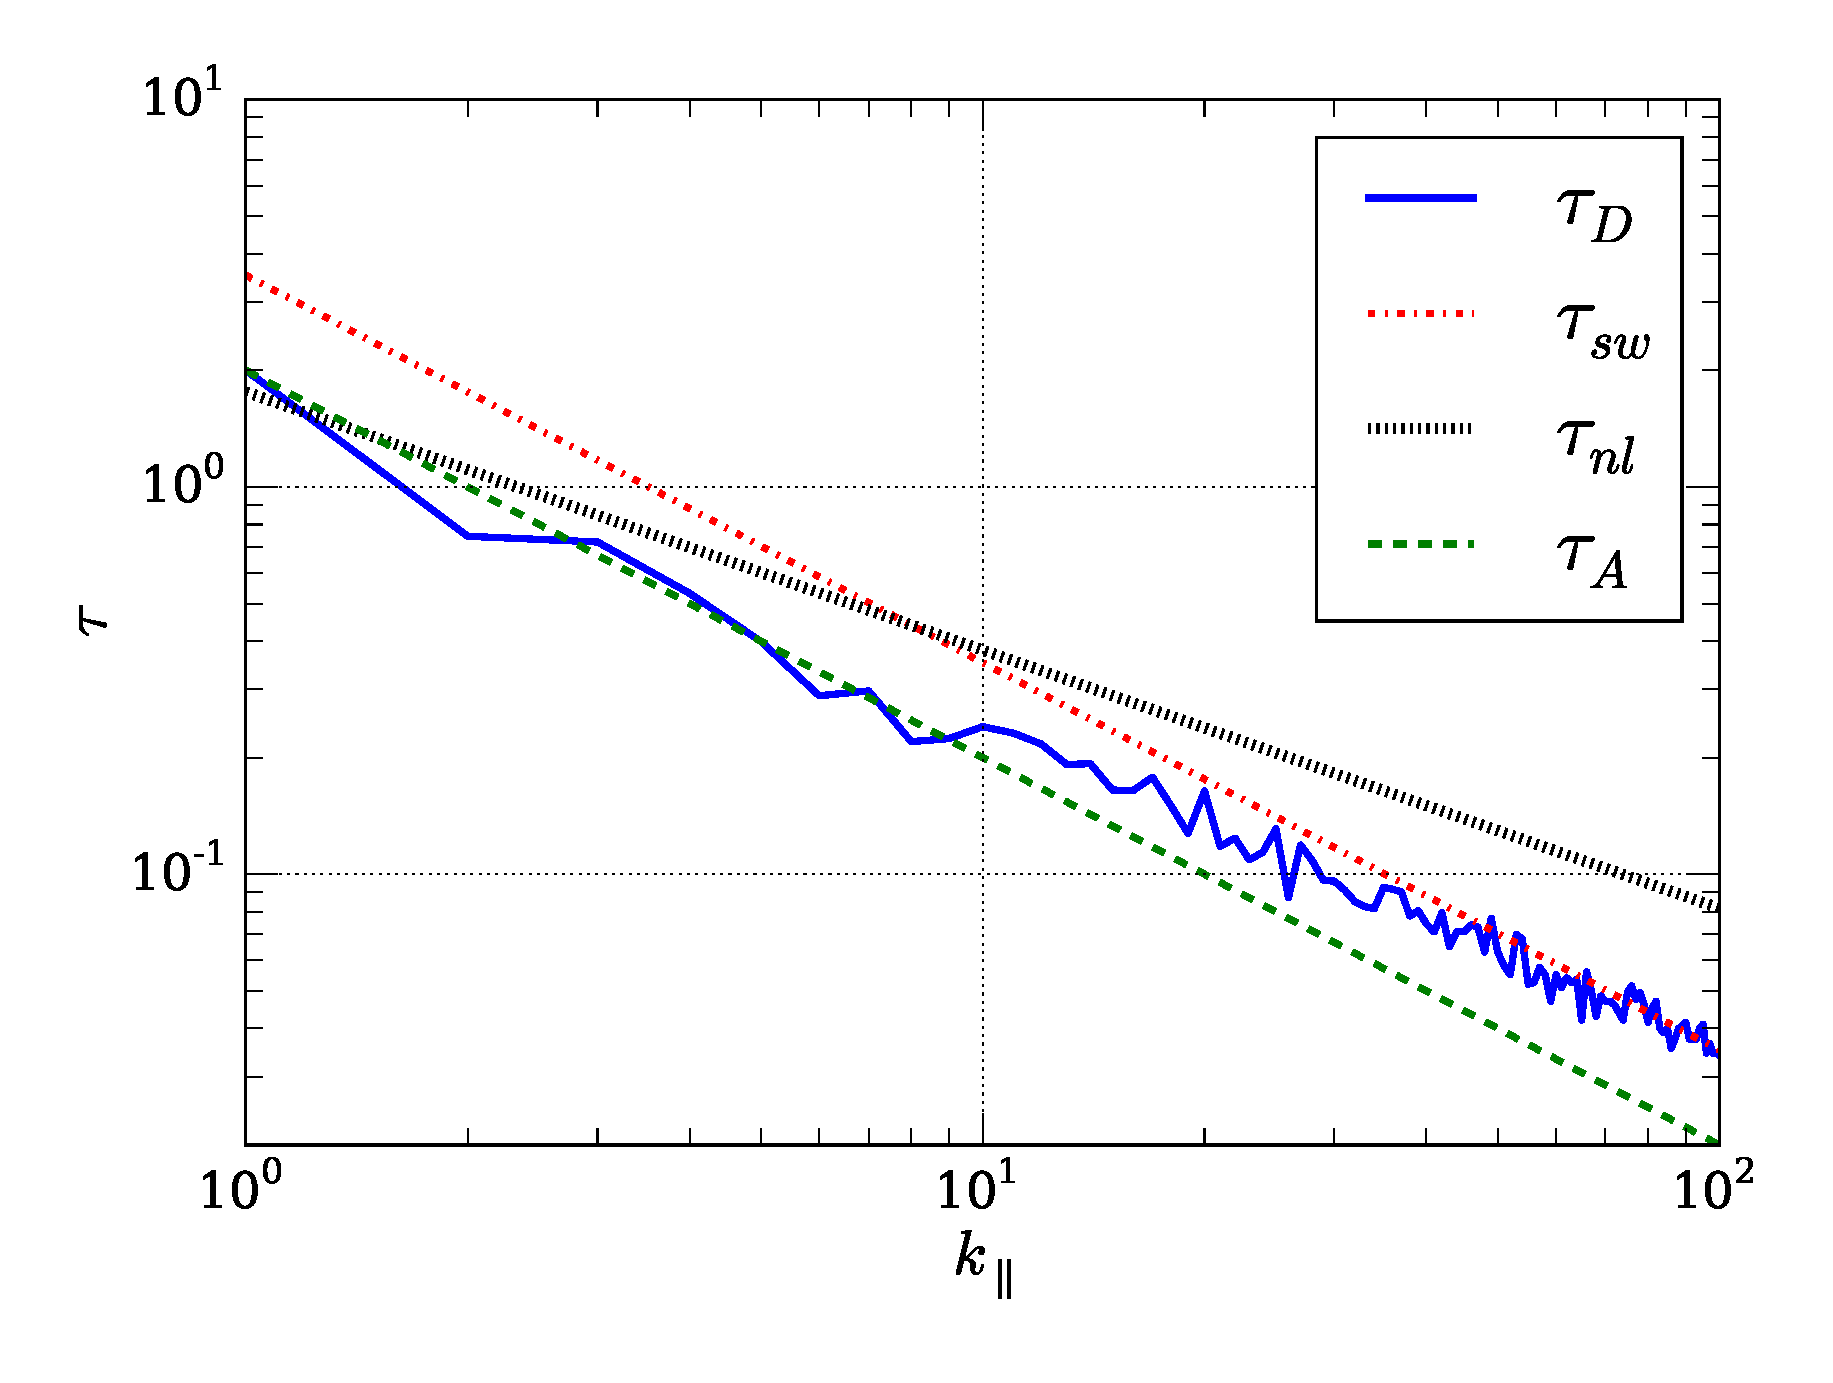
\includegraphics[width=0.76\columnwidth]{P1/fig5_B1_b_kperp_0.eps}
      \end{center}
    \end{minipage}
    \column{0.5\textwidth}
    \begin{minipage}[t]{1\textwidth}
      \begin{center}
        $k_\perp = 10$\\
        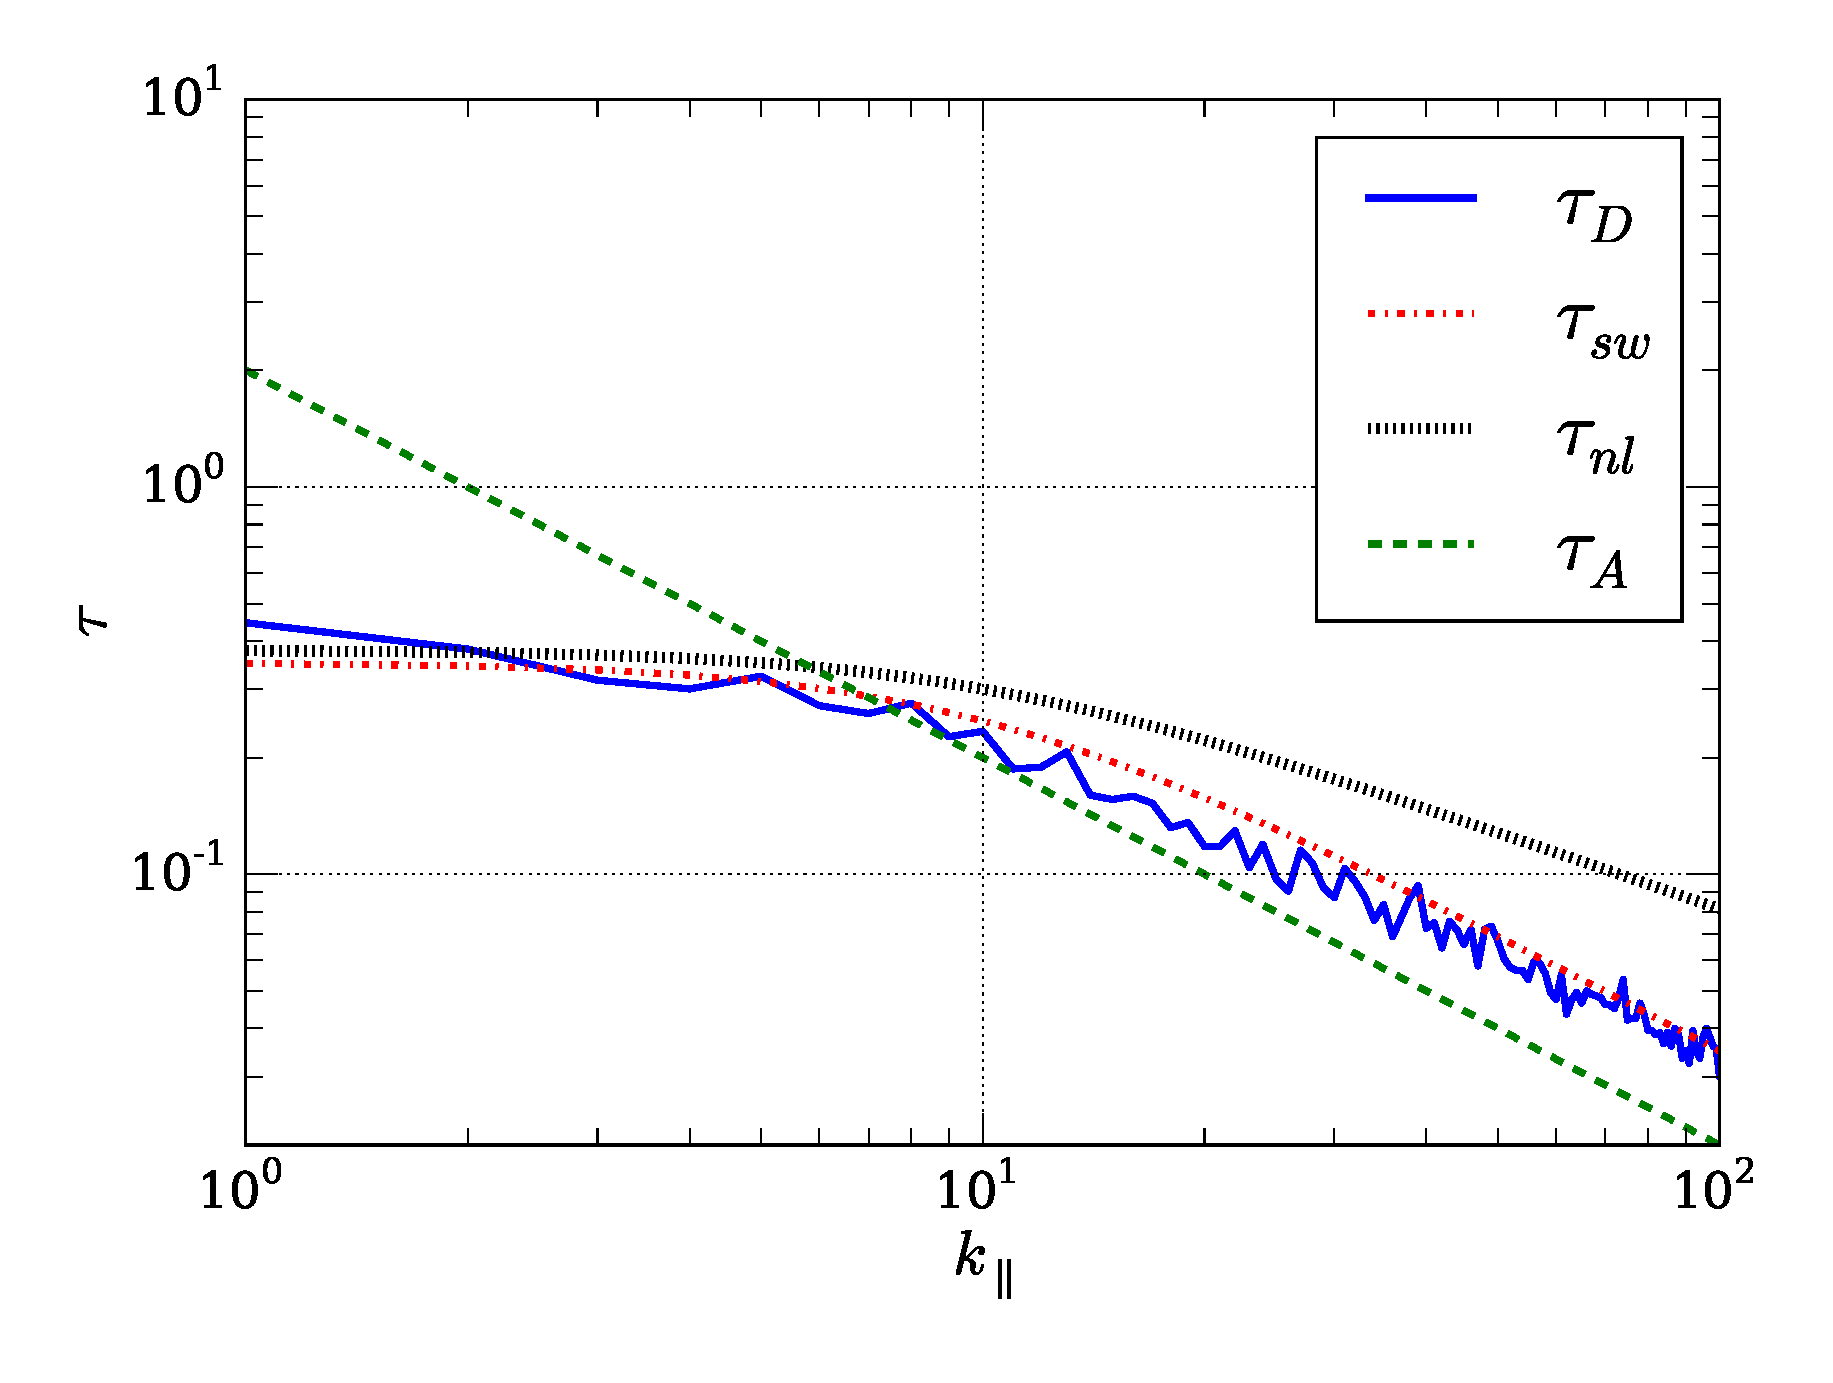
\includegraphics[width=0.76\columnwidth]{P1/fig5_B1_b_kperp_10.eps}
      \end{center}
    \end{minipage}
  \end{columns}
  \vspace{-0.5cm}
  \begin{center}
    $k_\perp = 20$\\
    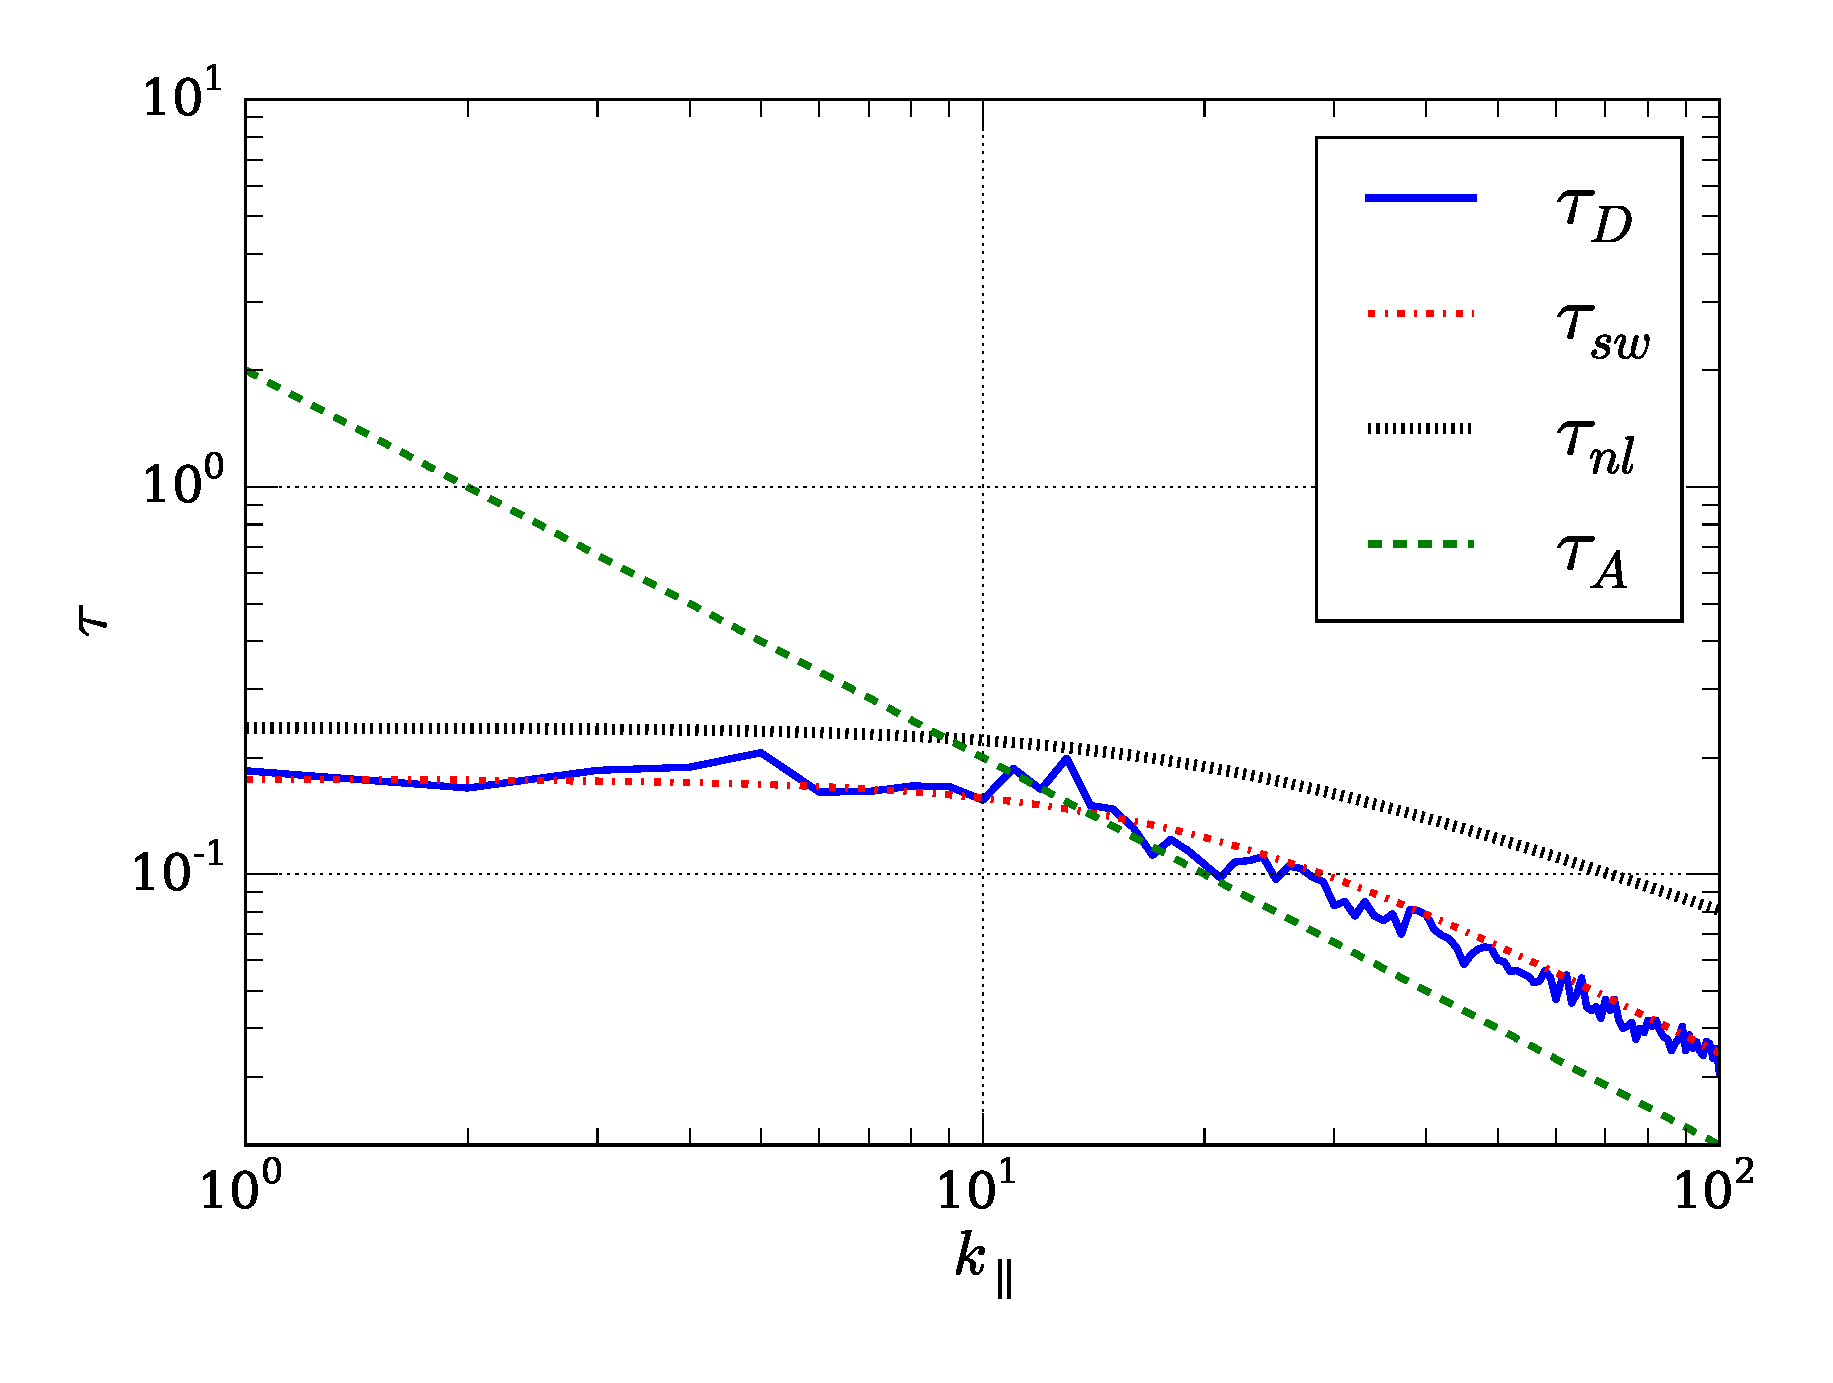
\includegraphics[width=0.38\columnwidth]{P1/fig5_B1_b_kperp_20.eps} \\
  \end{center}
}
\note[itemize]{
\item En el caso general, \textit{sweeping} y Alfvén escalan como
  $k^{-1}$. Con campo guía, podemos usar que Alfvén sólo escala con
  $k_\parallel$.
\item \emph{sweeping} domina $k$ grande, y Alfvén $k$ chico.
}



\frame{\frametitle{Tiempos de descorrelación}
  {\Large \underline{Tiempos de descorrelación: $B_0=1$ y $k_\parallel = k_0$}}
  \begin{columns}
    \column{0.5\textwidth}
    \begin{minipage}[t]{1\textwidth}
      \begin{center}
        $k_\parallel = 0$\\
        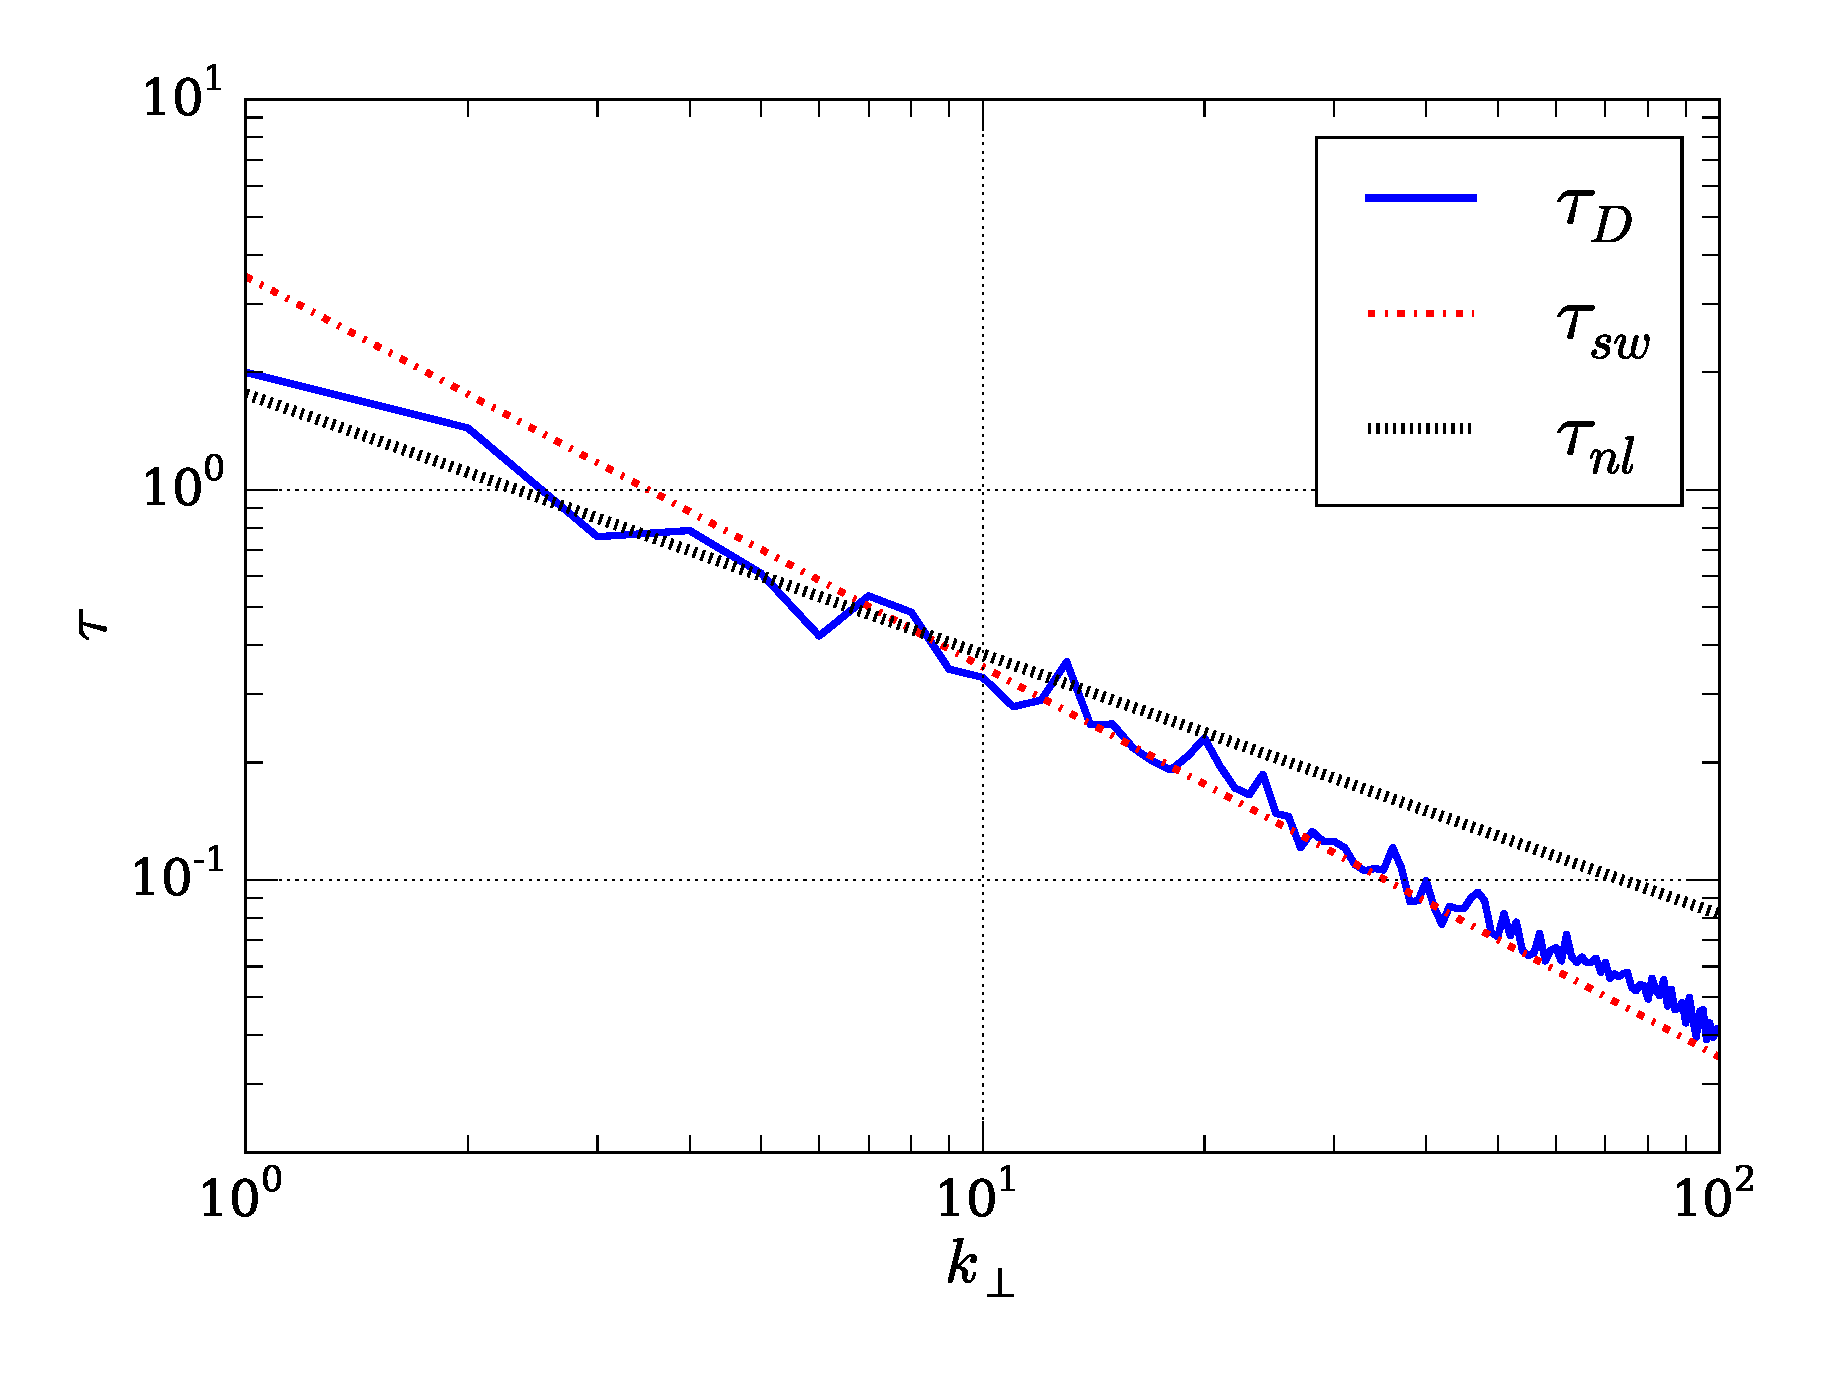
\includegraphics[width=0.76\columnwidth]{P1/fig5_B1_b_kpara_0.eps}
      \end{center}
    \end{minipage}
    \column{0.5\textwidth}
    \begin{minipage}[t]{1\textwidth}
      \begin{center}
        $k_\parallel = 10$\\
        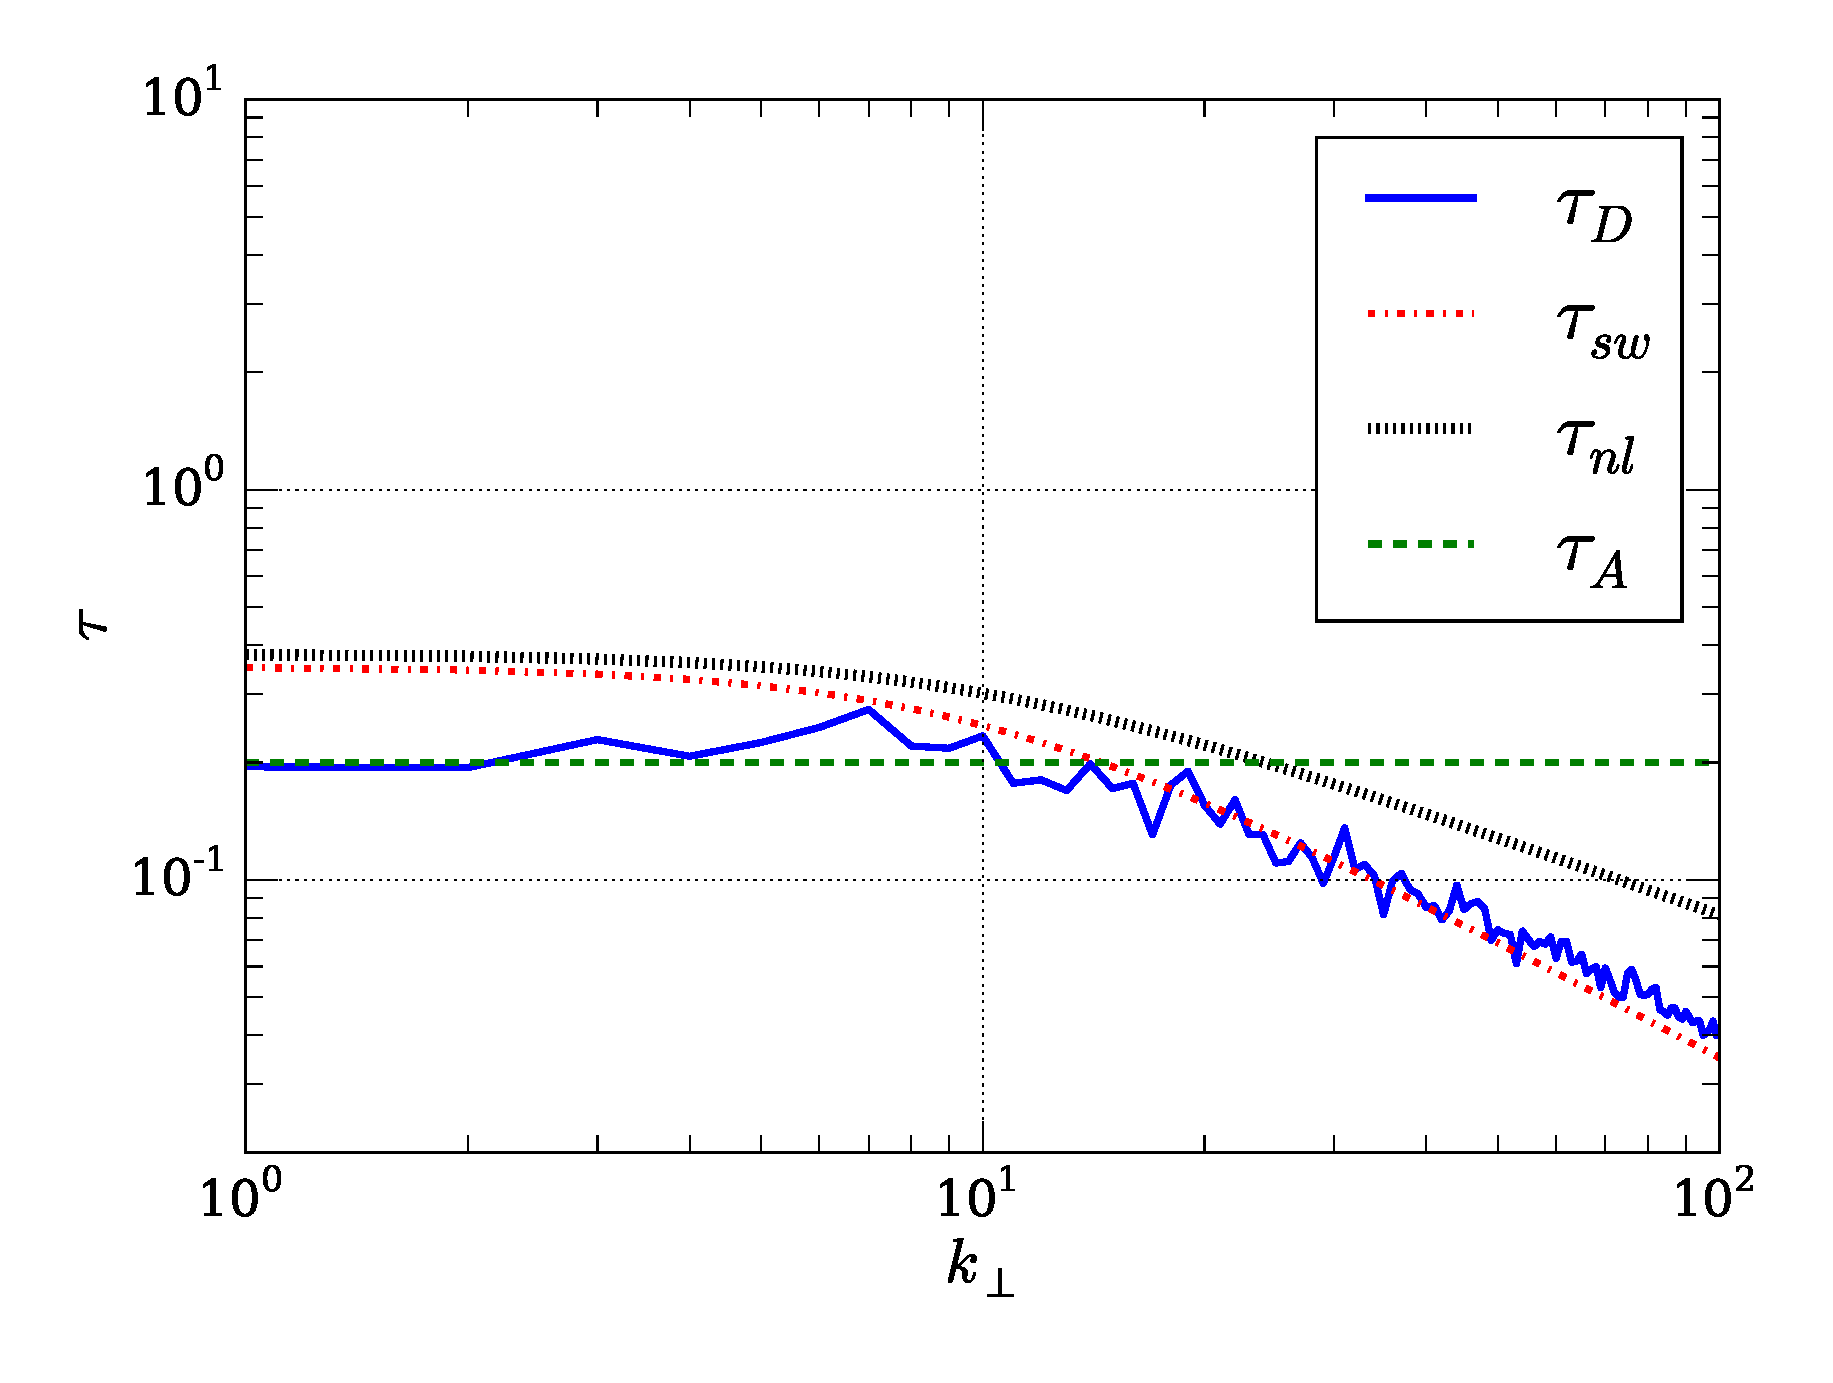
\includegraphics[width=0.76\columnwidth]{P1/fig5_B1_b_kpara_10.eps}
      \end{center}
    \end{minipage}
  \end{columns}
  \vspace{-0.5cm}
  \begin{center}
    $k_\parallel = 20$\\
    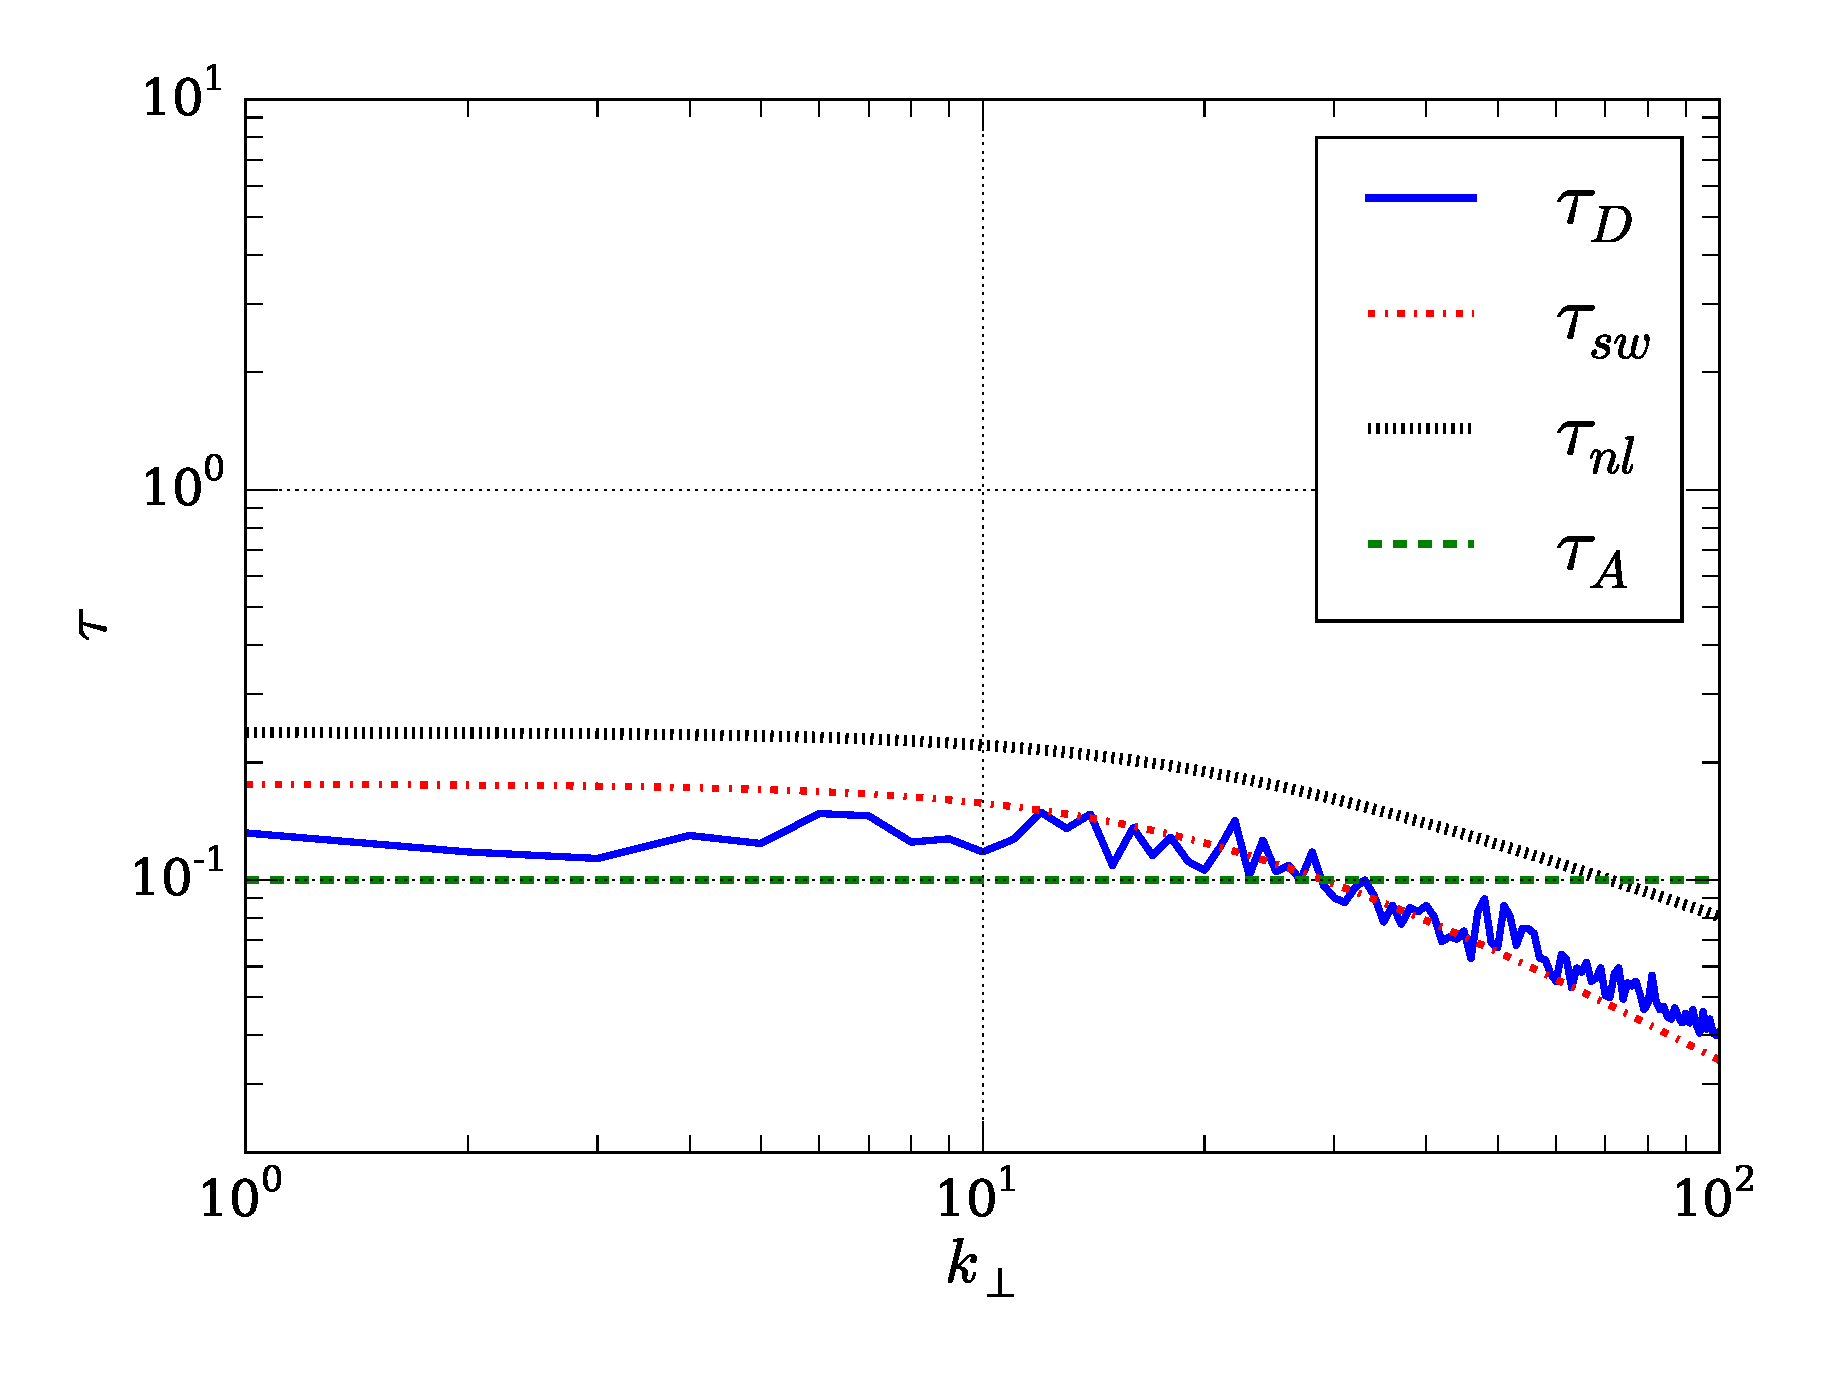
\includegraphics[width=0.38\columnwidth]{P1/fig5_B1_b_kpara_20.eps} \\
  \end{center}
}


\frame{\frametitle{Tiempos de descorrelación}
  {\Large \underline{Tiempos de descorrelación: $B_0=0.25$ y $k_\perp = k_0$}}
  \begin{columns}
    \column{0.5\textwidth}
    \begin{minipage}[t]{1\textwidth}
      \begin{center}
        $k_\perp = 0$\\
        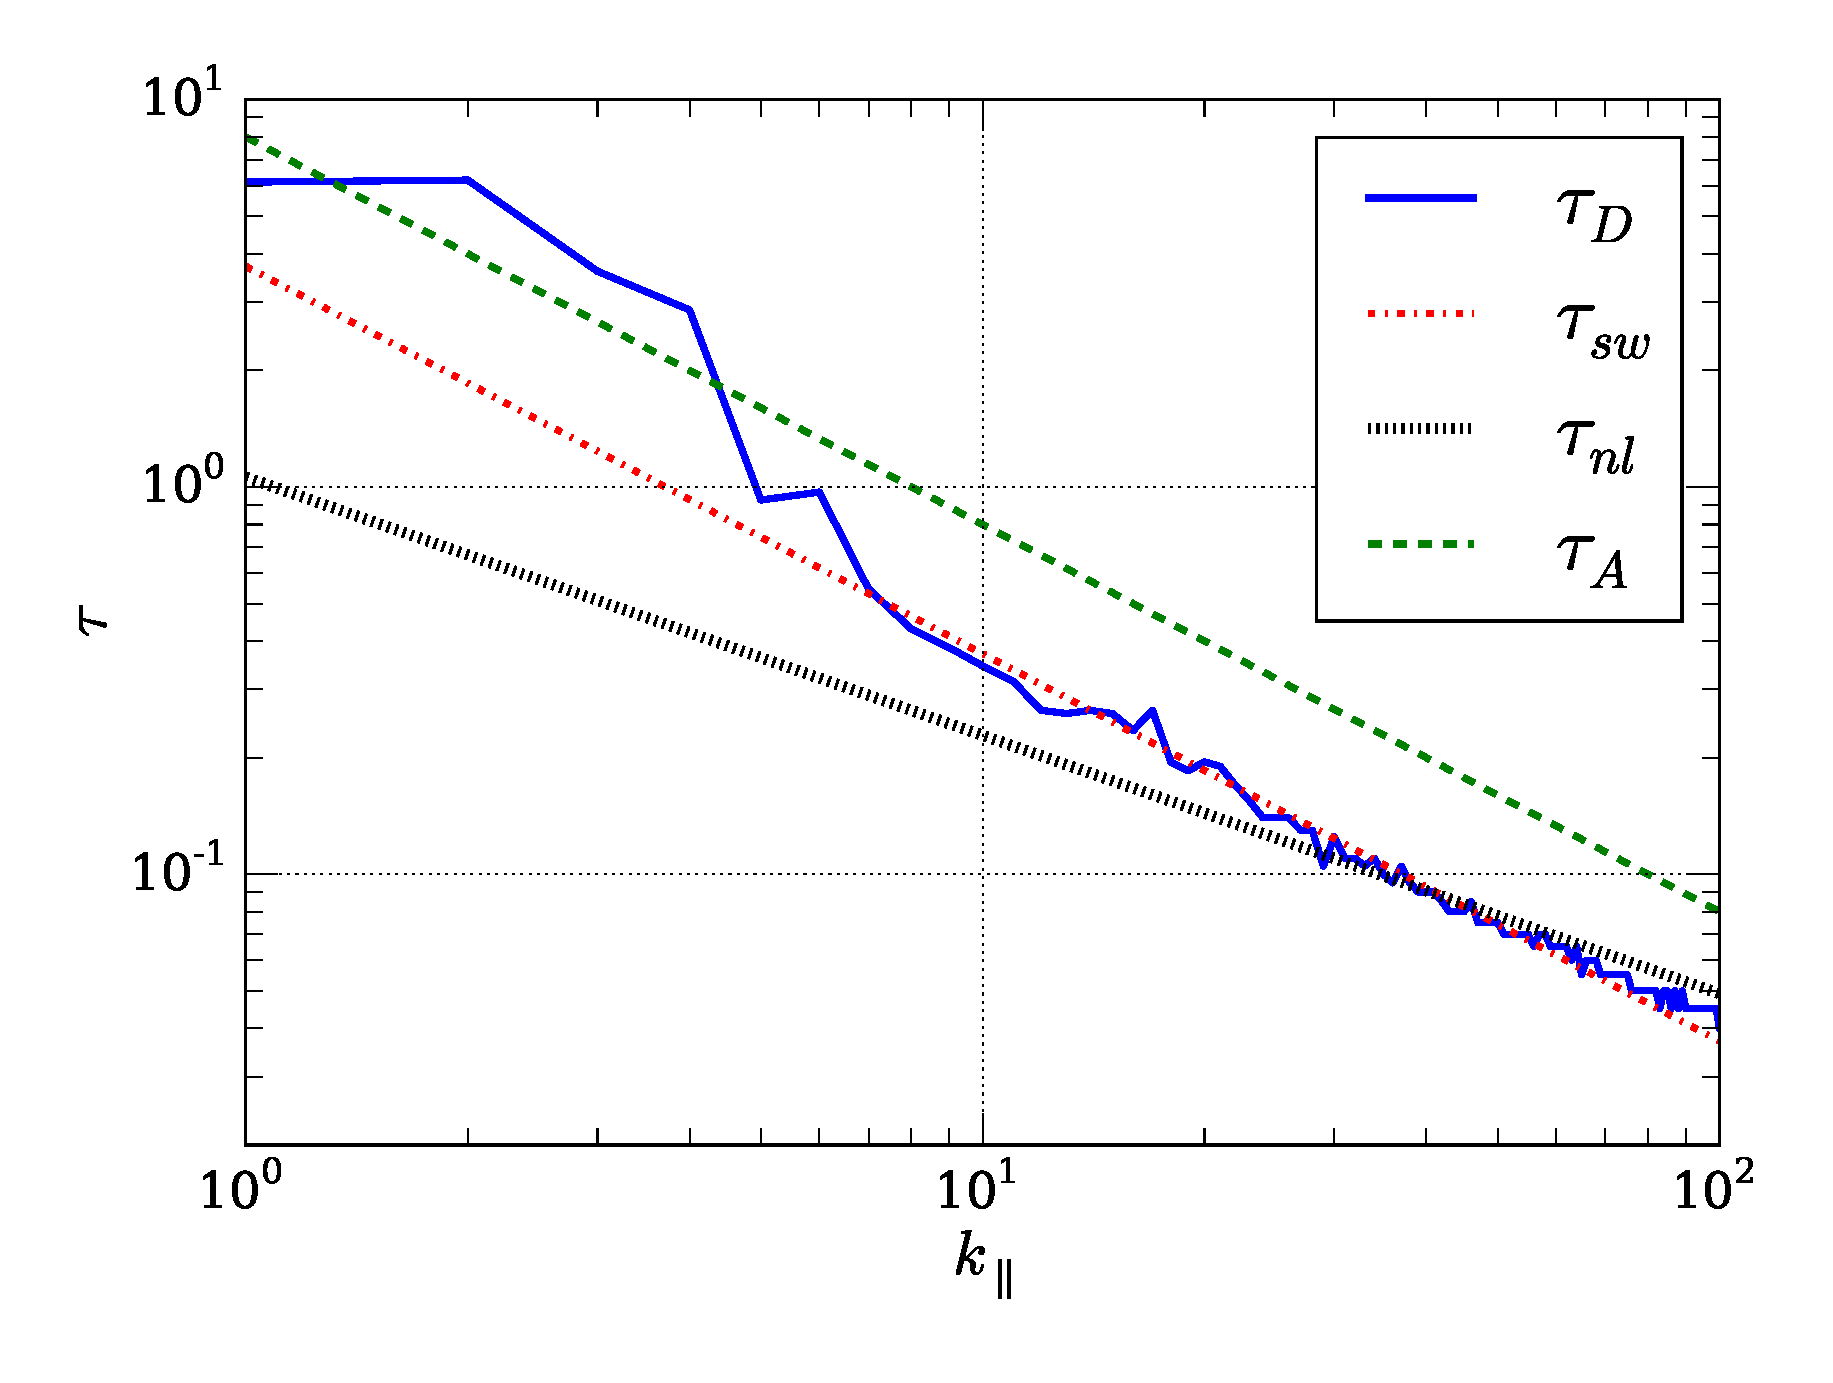
\includegraphics[width=0.76\columnwidth]{P1/fig5_B025_b_kperp_0.eps}
      \end{center}
    \end{minipage}
    \column{0.5\textwidth}
    \begin{minipage}[t]{1\textwidth}
      \begin{center}
        $k_\perp = 10$\\
        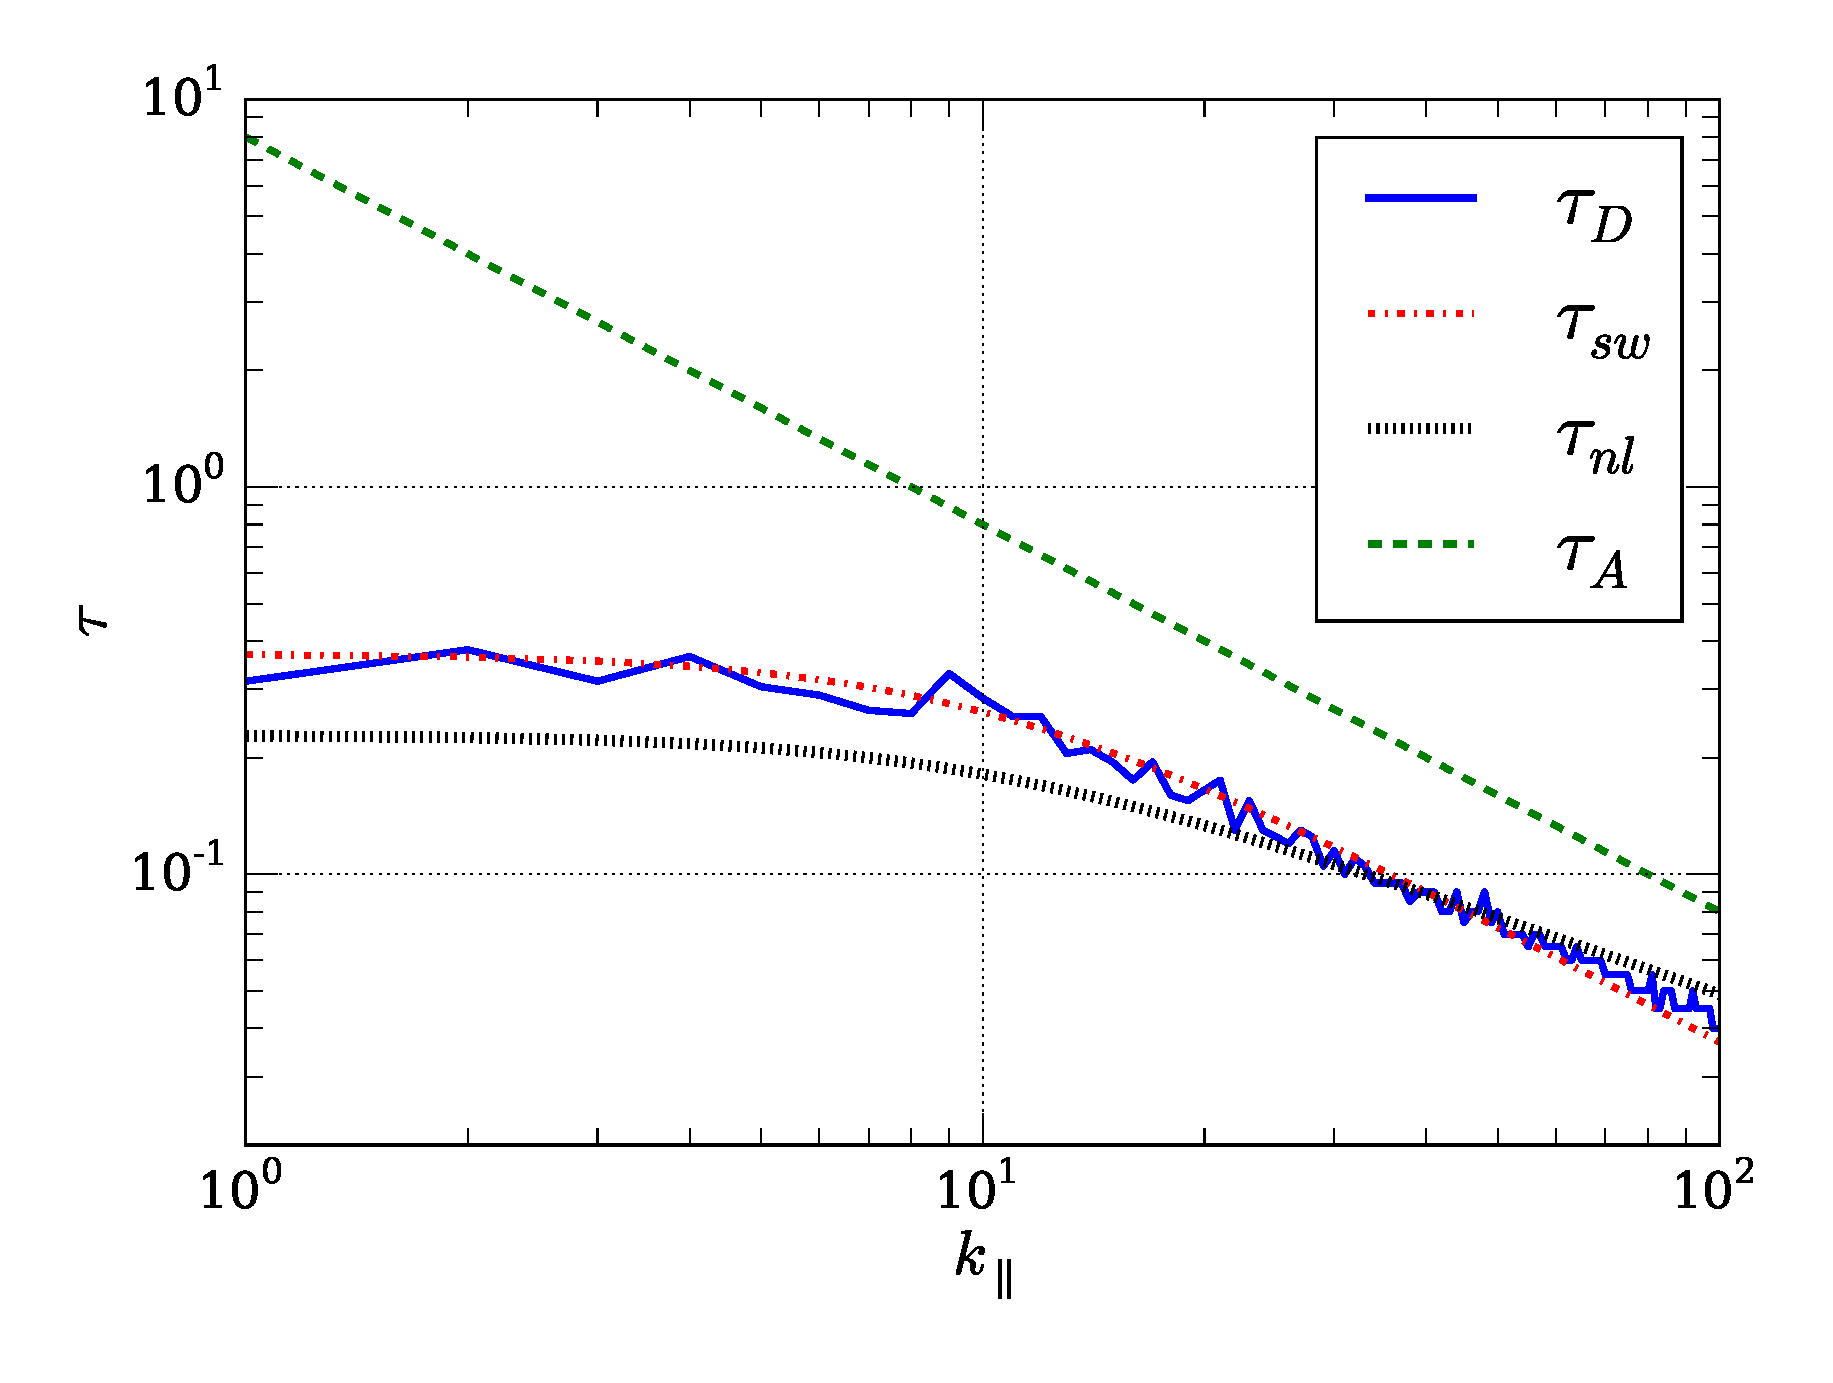
\includegraphics[width=0.76\columnwidth]{P1/fig5_B025_b_kperp_10.eps}
      \end{center}
    \end{minipage}
  \end{columns}
  \vspace{-0.5cm}
  \begin{center}
    $k_\perp = 20$\\
    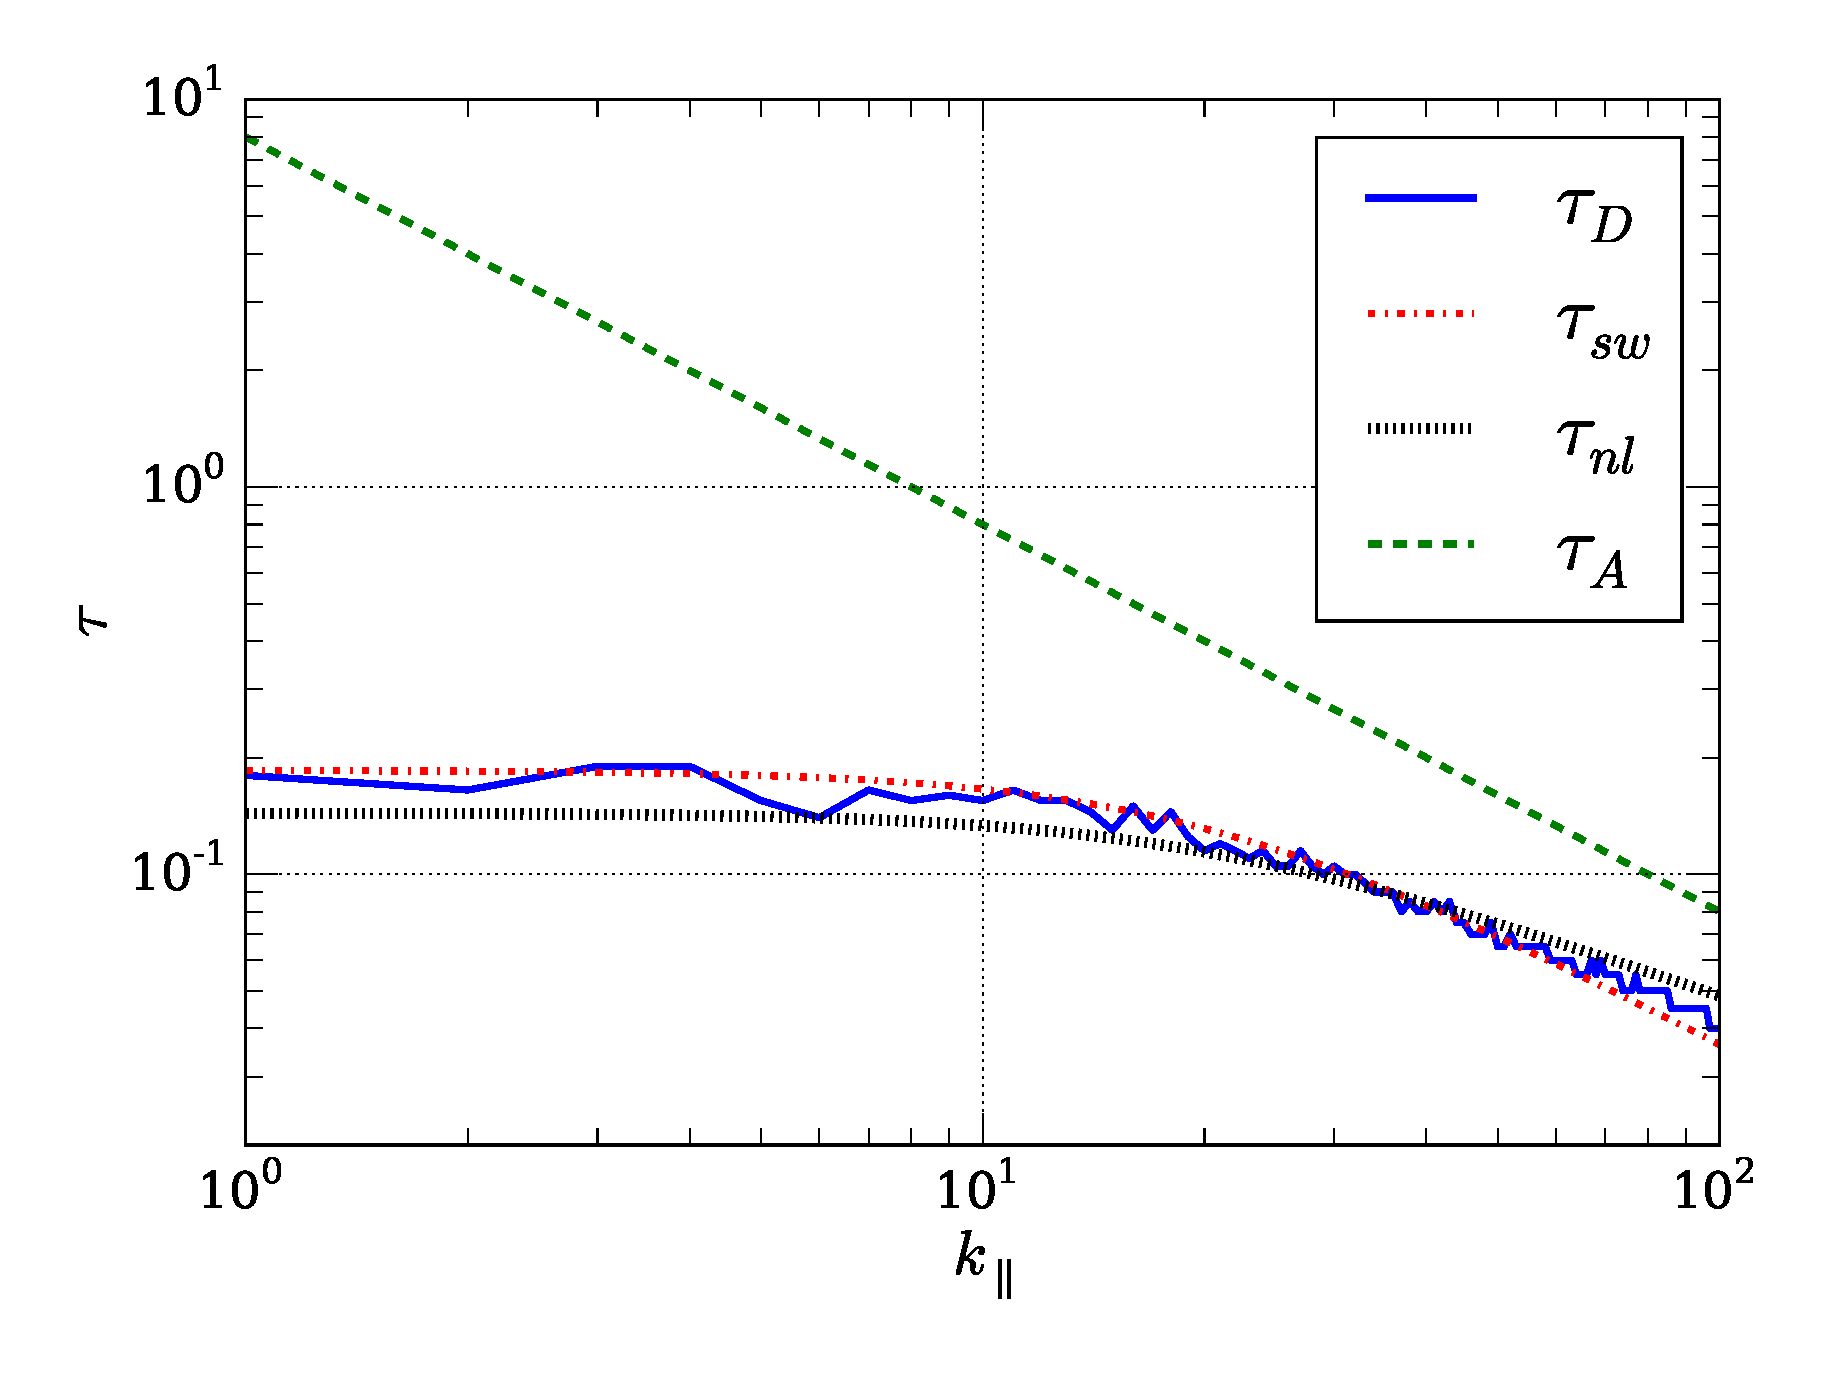
\includegraphics[width=0.38\columnwidth]{P1/fig5_B025_b_kperp_20.eps} \\
  \end{center}
}
\note[itemize]{
\item Tiempos de descorrelación más cercanos al tiempo de
  \textit{sweeping}. Consistente con el resultado del espectro
  energético.
}


\frame{\frametitle{Tiempos de descorrelación}
  {\Large \underline{Tiempos de descorrelación: $B_0=0.25$ y $k_\parallel = k_0$}}
  \begin{columns}
    \column{0.5\textwidth}
    \begin{minipage}[t]{1\textwidth}
      \begin{center}
        $k_\parallel = 0$\\
        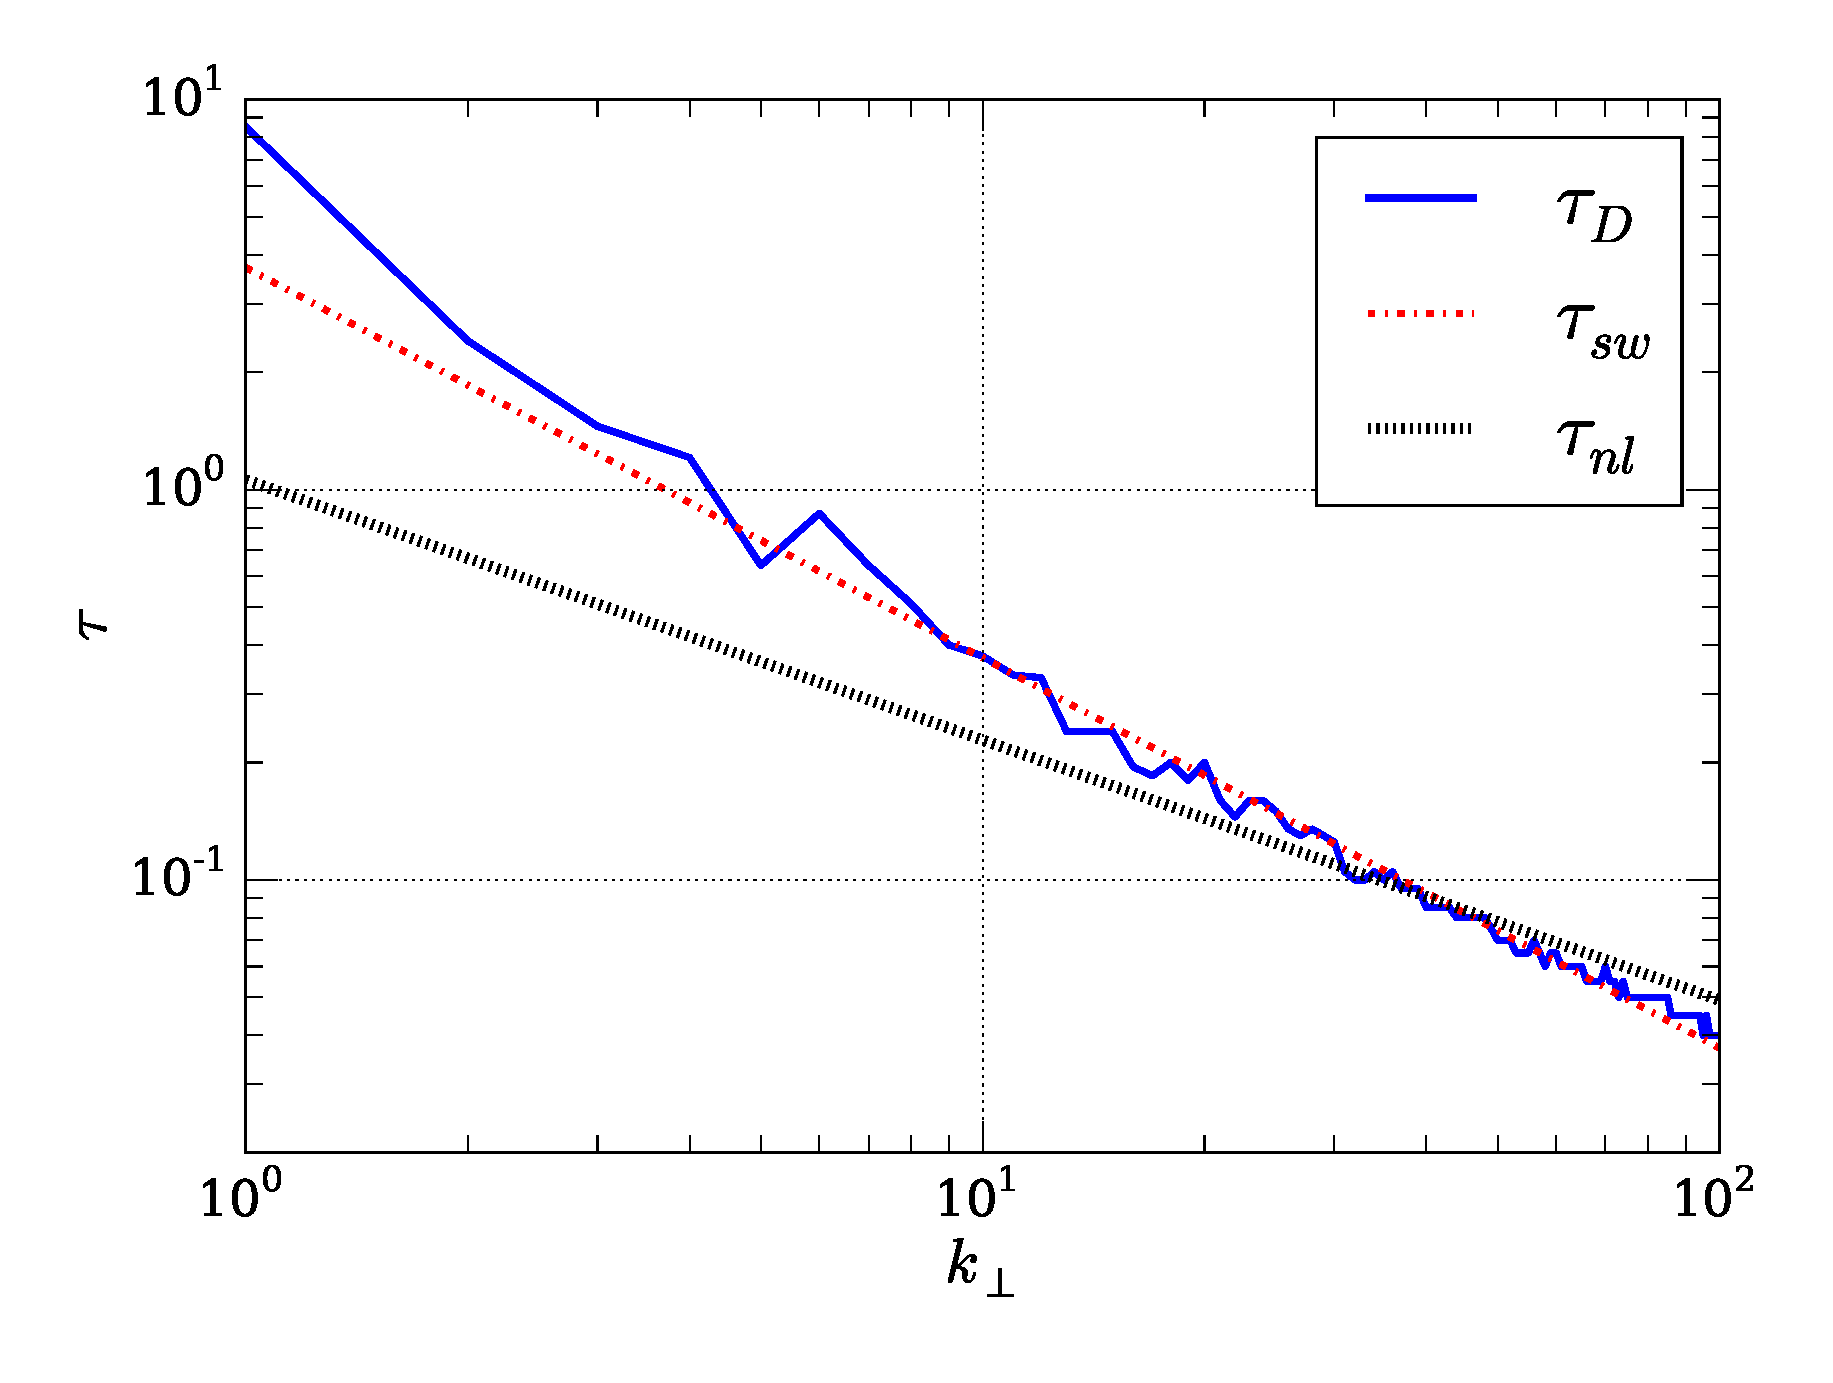
\includegraphics[width=0.76\columnwidth]{P1/fig5_B025_b_kpara_0.eps}
      \end{center}
    \end{minipage}
    \column{0.5\textwidth}
    \begin{minipage}[t]{1\textwidth}
      \begin{center}
        $k_\parallel = 10$\\
        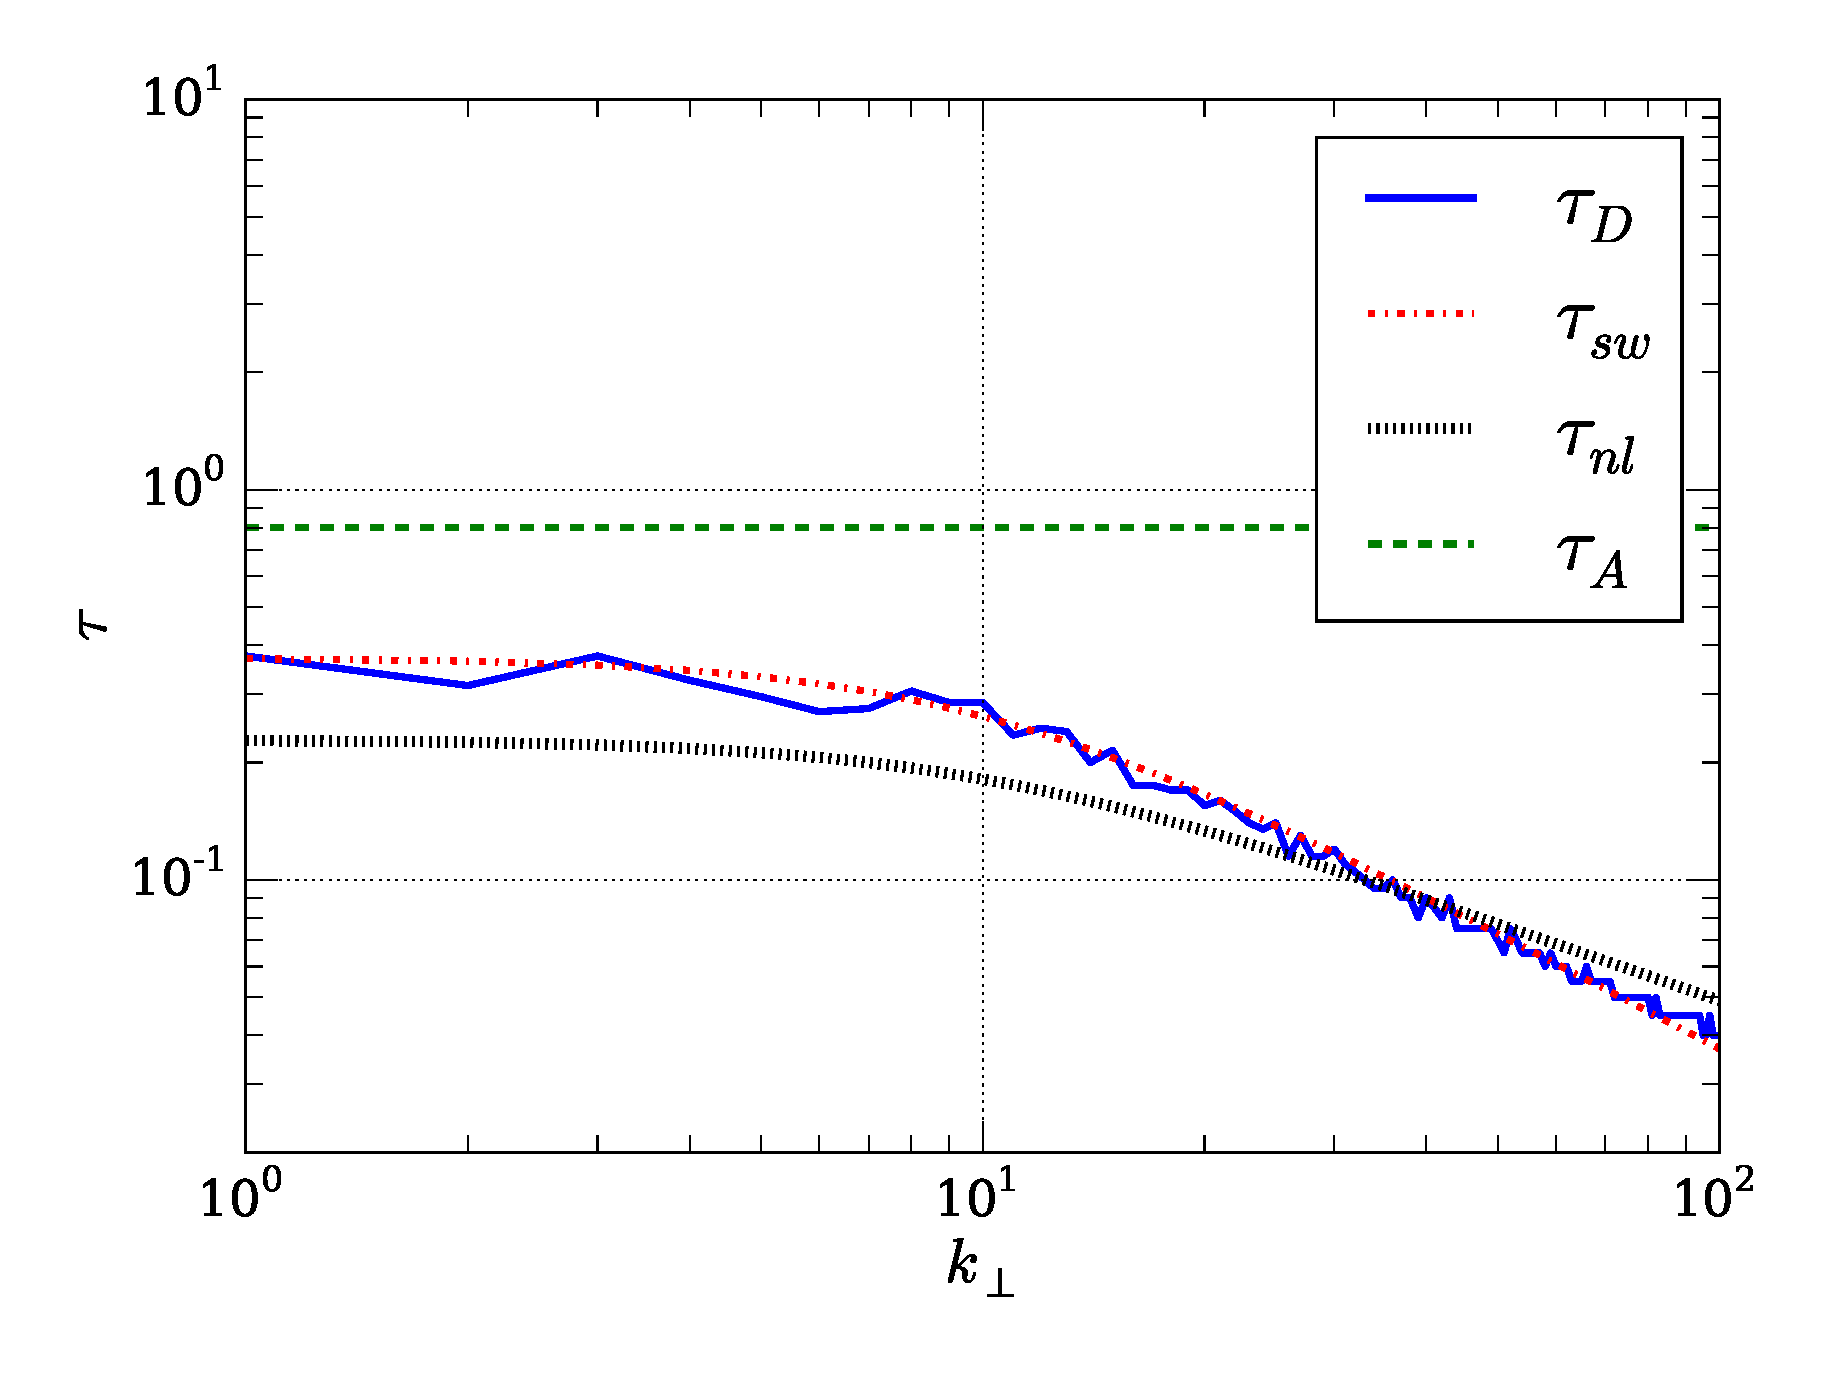
\includegraphics[width=0.76\columnwidth]{P1/fig5_B025_b_kpara_10.eps}
      \end{center}
    \end{minipage}
  \end{columns}
  \vspace{-0.5cm}
  \begin{center}
    $k_\parallel = 20$\\
    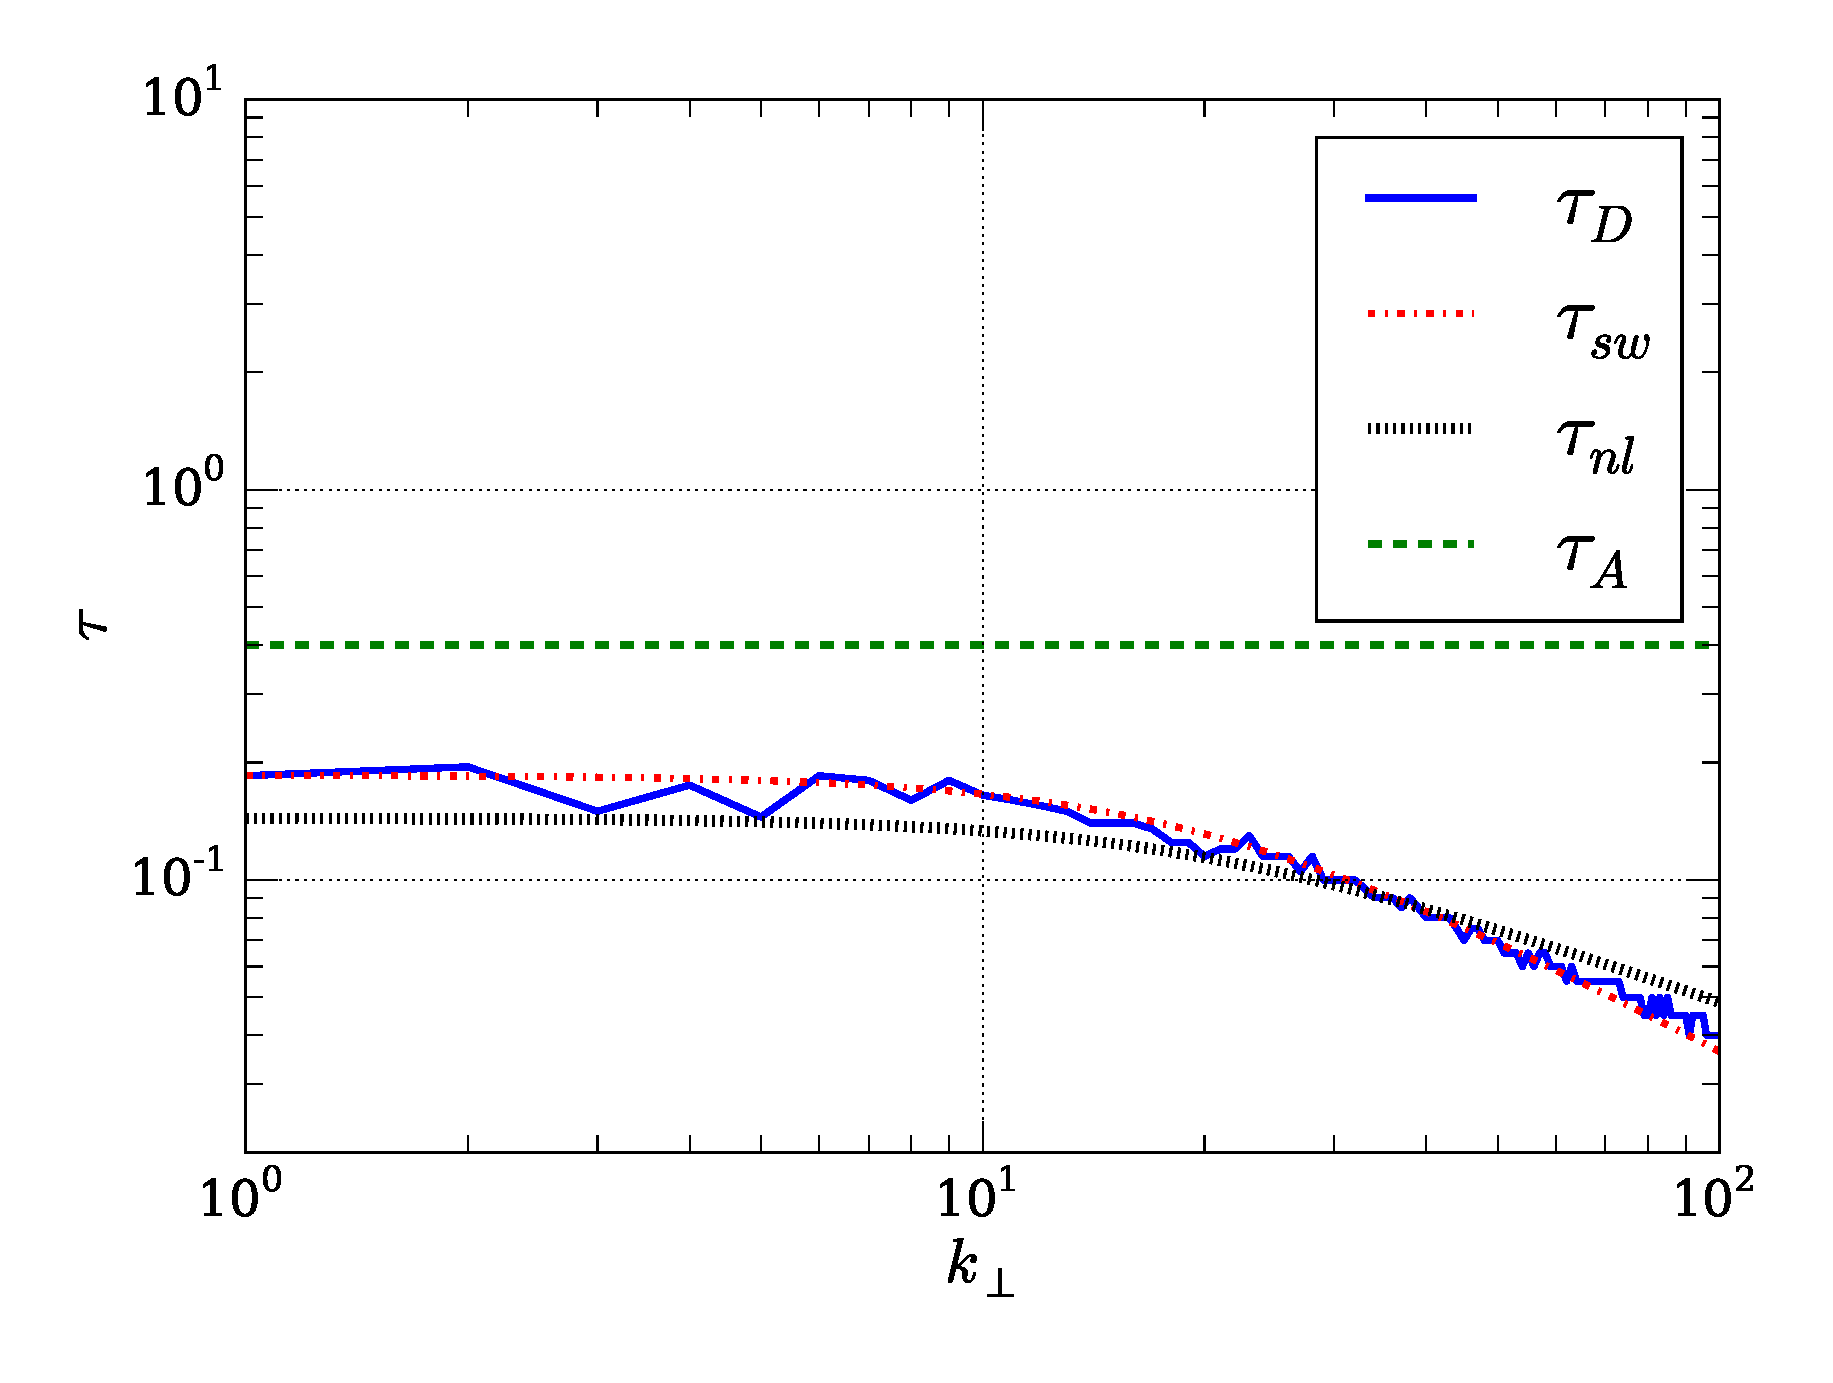
\includegraphics[width=0.38\columnwidth]{P1/fig5_B025_b_kpara_20.eps} \\
  \end{center}
}
\note[itemize]{
\item 
}


\frame{\frametitle{Tiempos de descorrelación}
  {\Large \underline{Tiempos de descorrelación: $B_0=8$ y $k_\perp = k_0$}}
  \begin{columns}
    \column{0.5\textwidth}
    \begin{minipage}[t]{1\textwidth}
      \begin{center}
        $k_\perp = 0$\\
        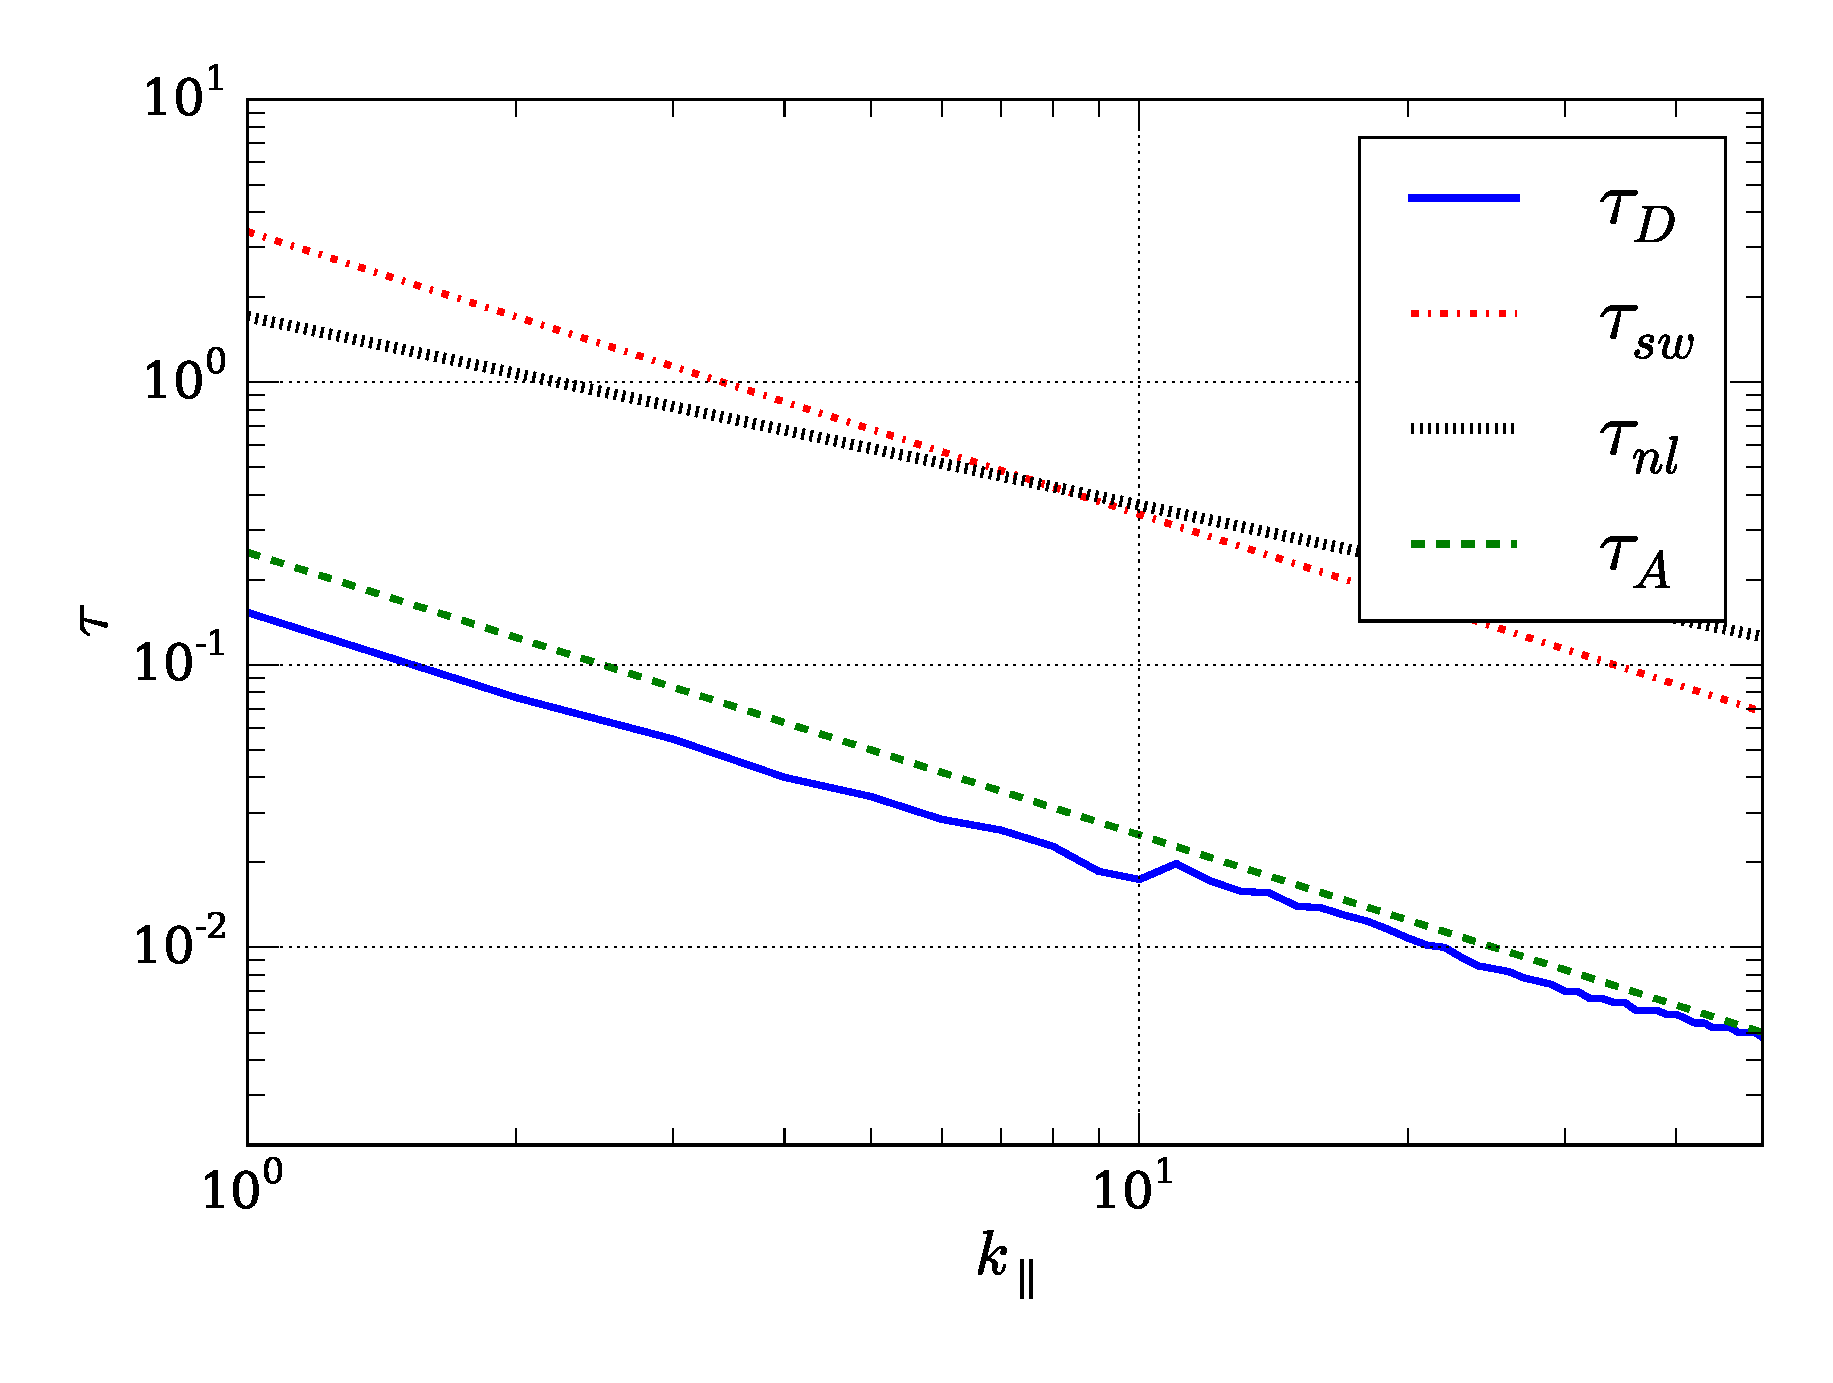
\includegraphics[width=0.76\columnwidth]{P1/fig5_B8_b_kperp_0.eps}
      \end{center}
    \end{minipage}
    \column{0.5\textwidth}
    \begin{minipage}[t]{1\textwidth}
      \begin{center}
        $k_\perp = 10$\\
        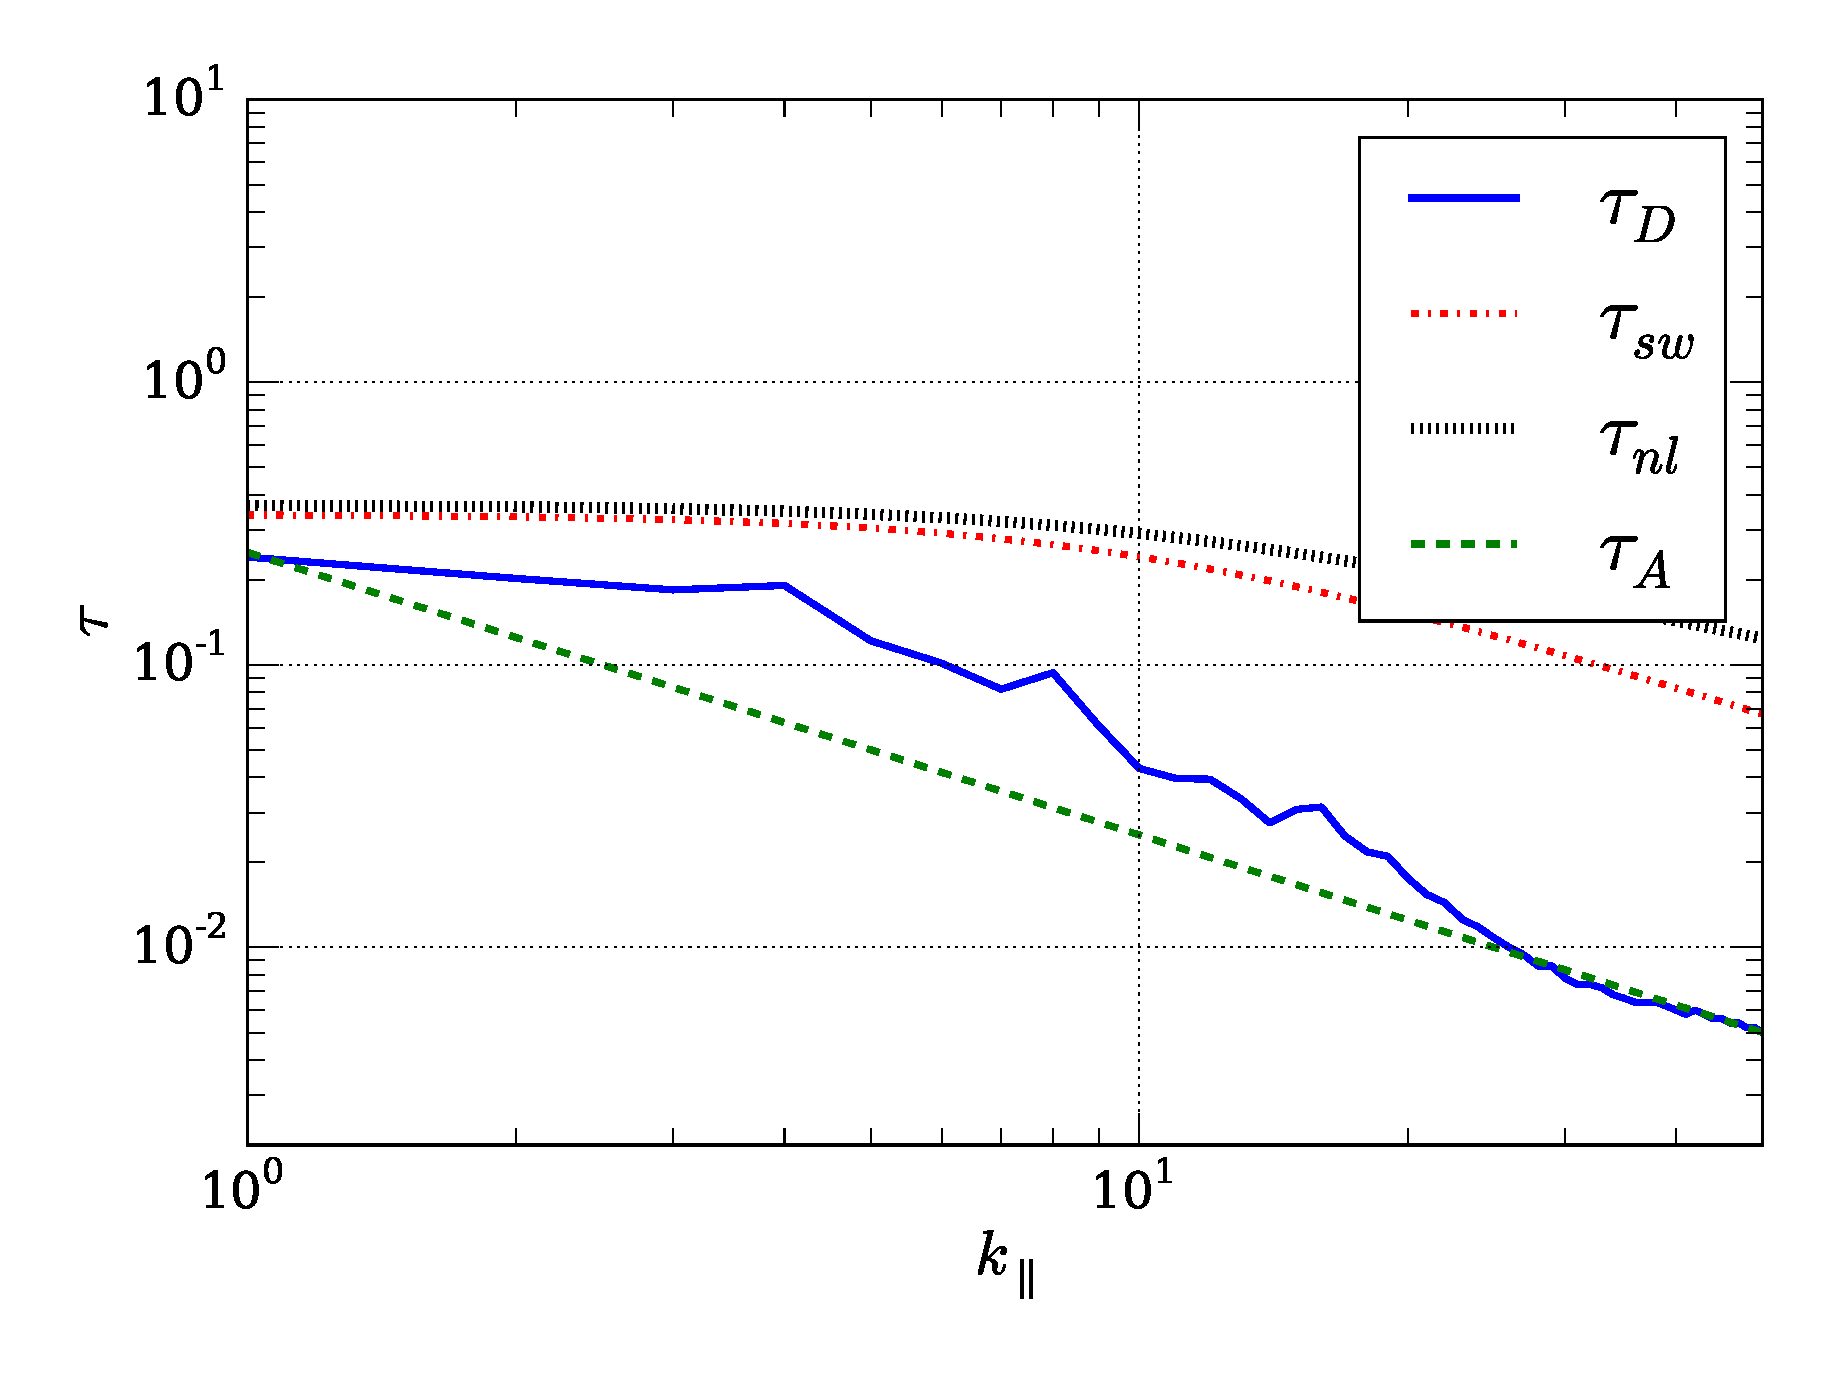
\includegraphics[width=0.76\columnwidth]{P1/fig5_B8_b_kperp_10.eps}
      \end{center}
    \end{minipage}
  \end{columns}
  \vspace{-0.5cm}
  \begin{center}
    $k_\perp = 20$\\
    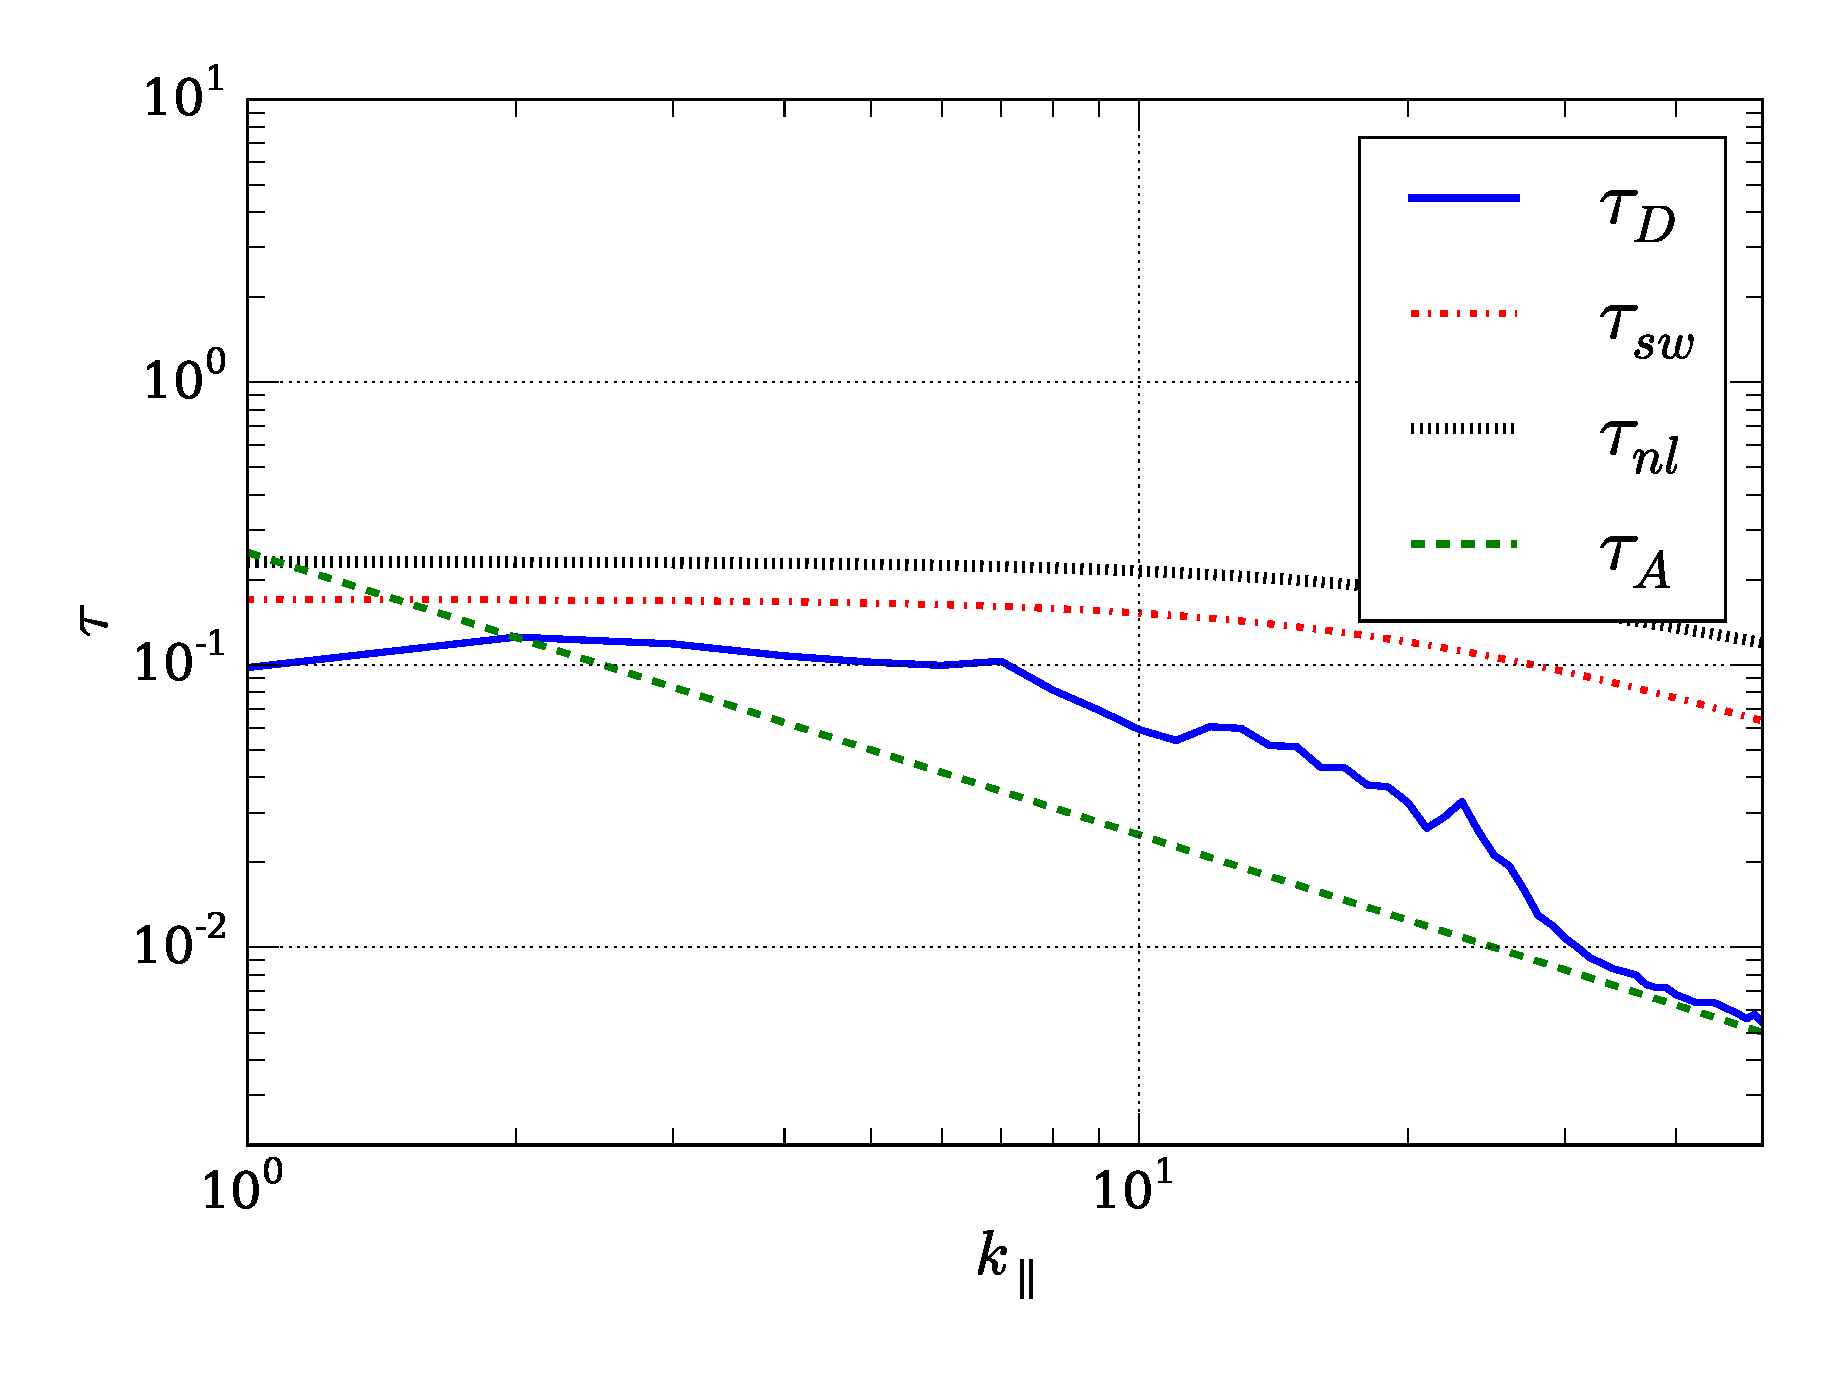
\includegraphics[width=0.38\columnwidth]{P1/fig5_B8_b_kperp_20.eps} \\
  \end{center}
}
\note[itemize]{
\item Para valores pequeños de $k_\perp$, el tiempo de Alfvén
  domina. Después, $\tau_D$ se acerca al \emph{sweeping}.
}




\frame{\frametitle{Tiempos de descorrelación}
  {\Large \underline{Tiempos de descorrelación: $B_0=8$ y $k_\parallel = k_0$}}
  \begin{columns}
    \column{0.5\textwidth}
    \begin{minipage}[t]{1\textwidth}
      \begin{center}
        $k_\parallel = 0$\\
        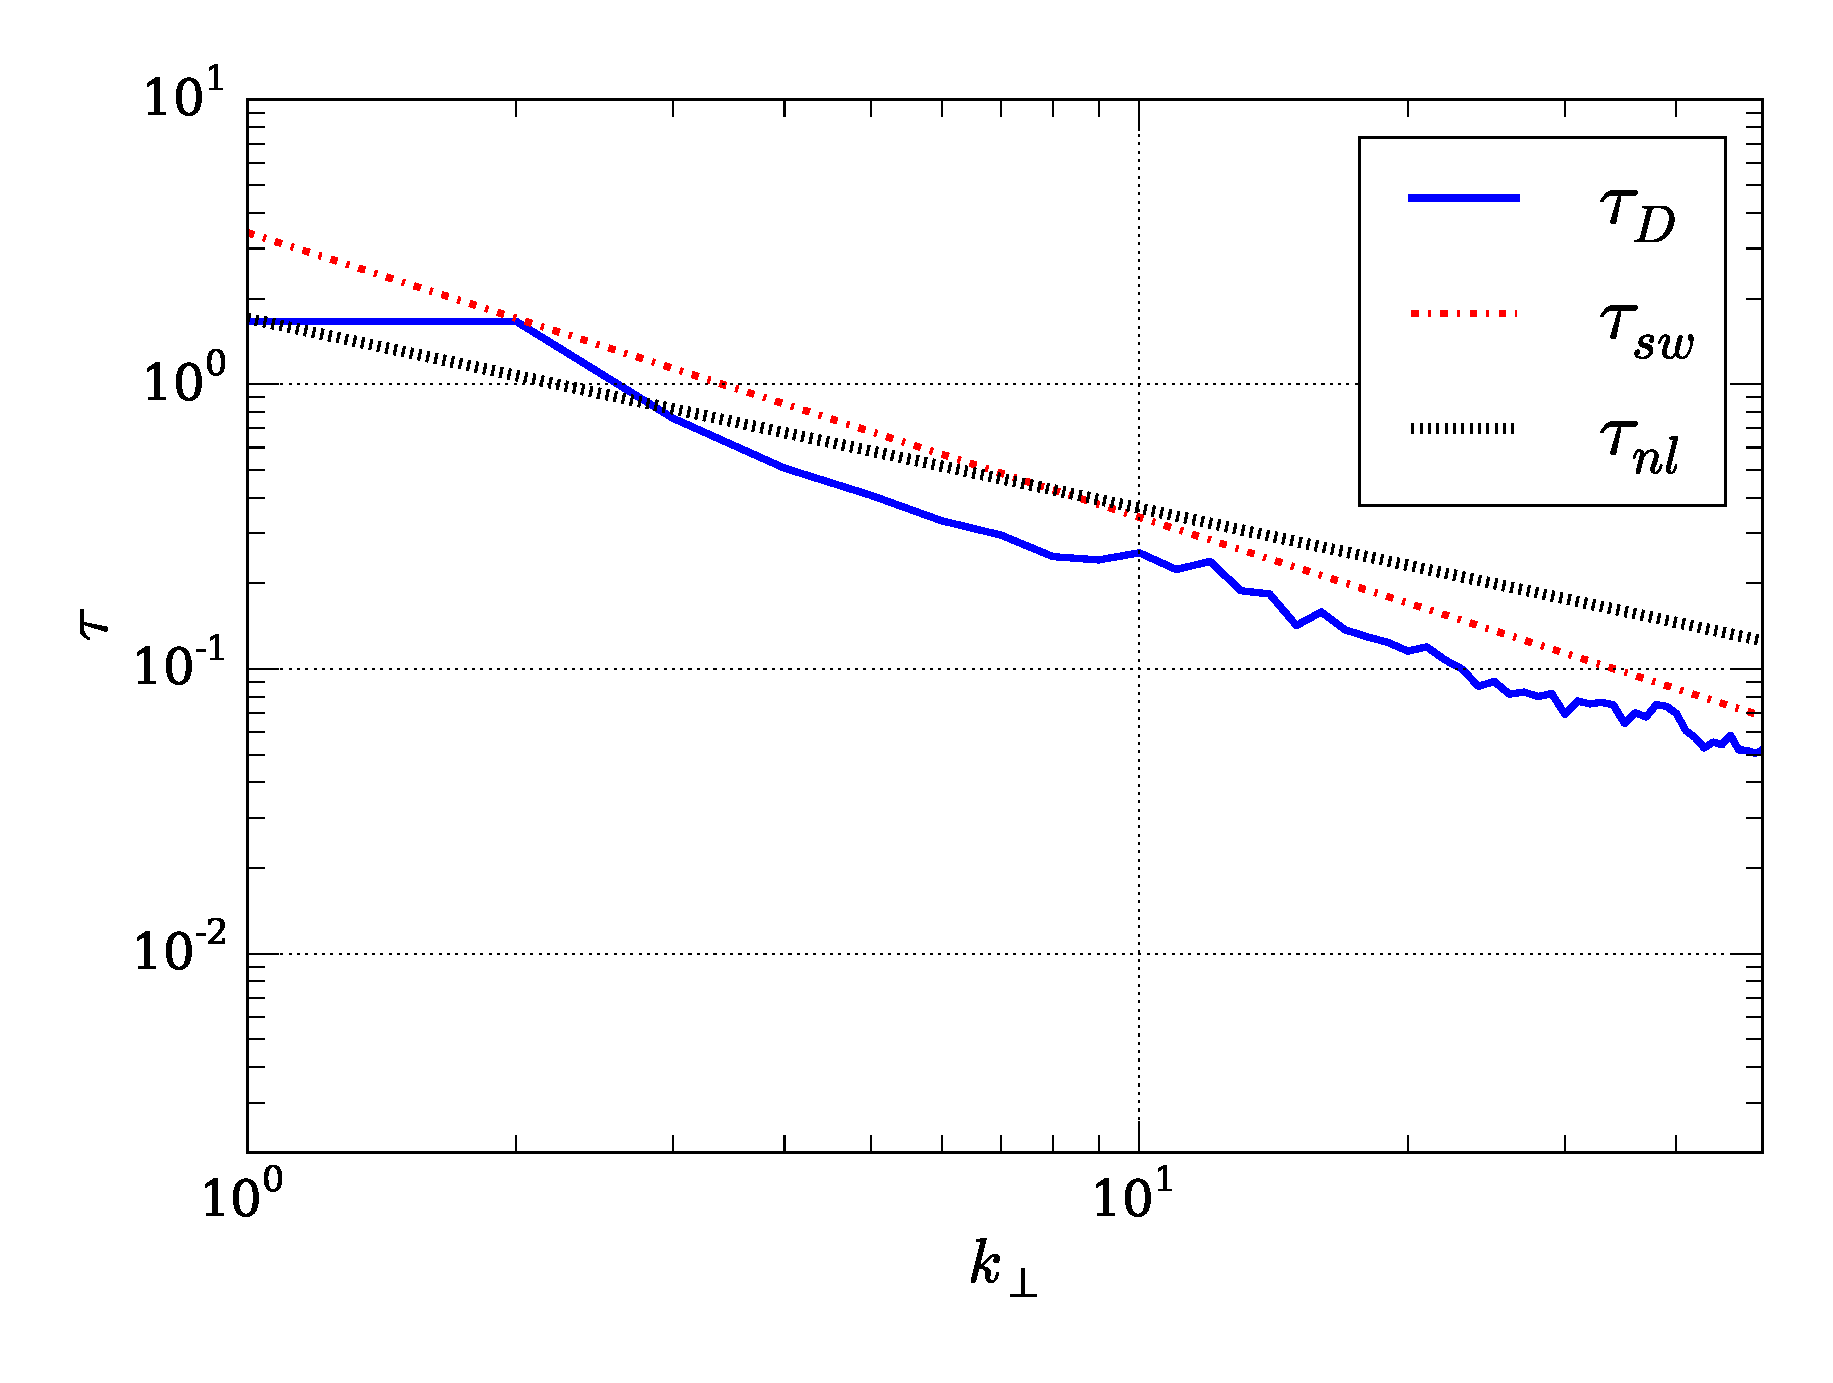
\includegraphics[width=0.76\columnwidth]{P1/fig5_B8_b_kpara_0.eps}
      \end{center}
    \end{minipage}
    \column{0.5\textwidth}
    \begin{minipage}[t]{1\textwidth}
      \begin{center}
        $k_\parallel = 10$\\
        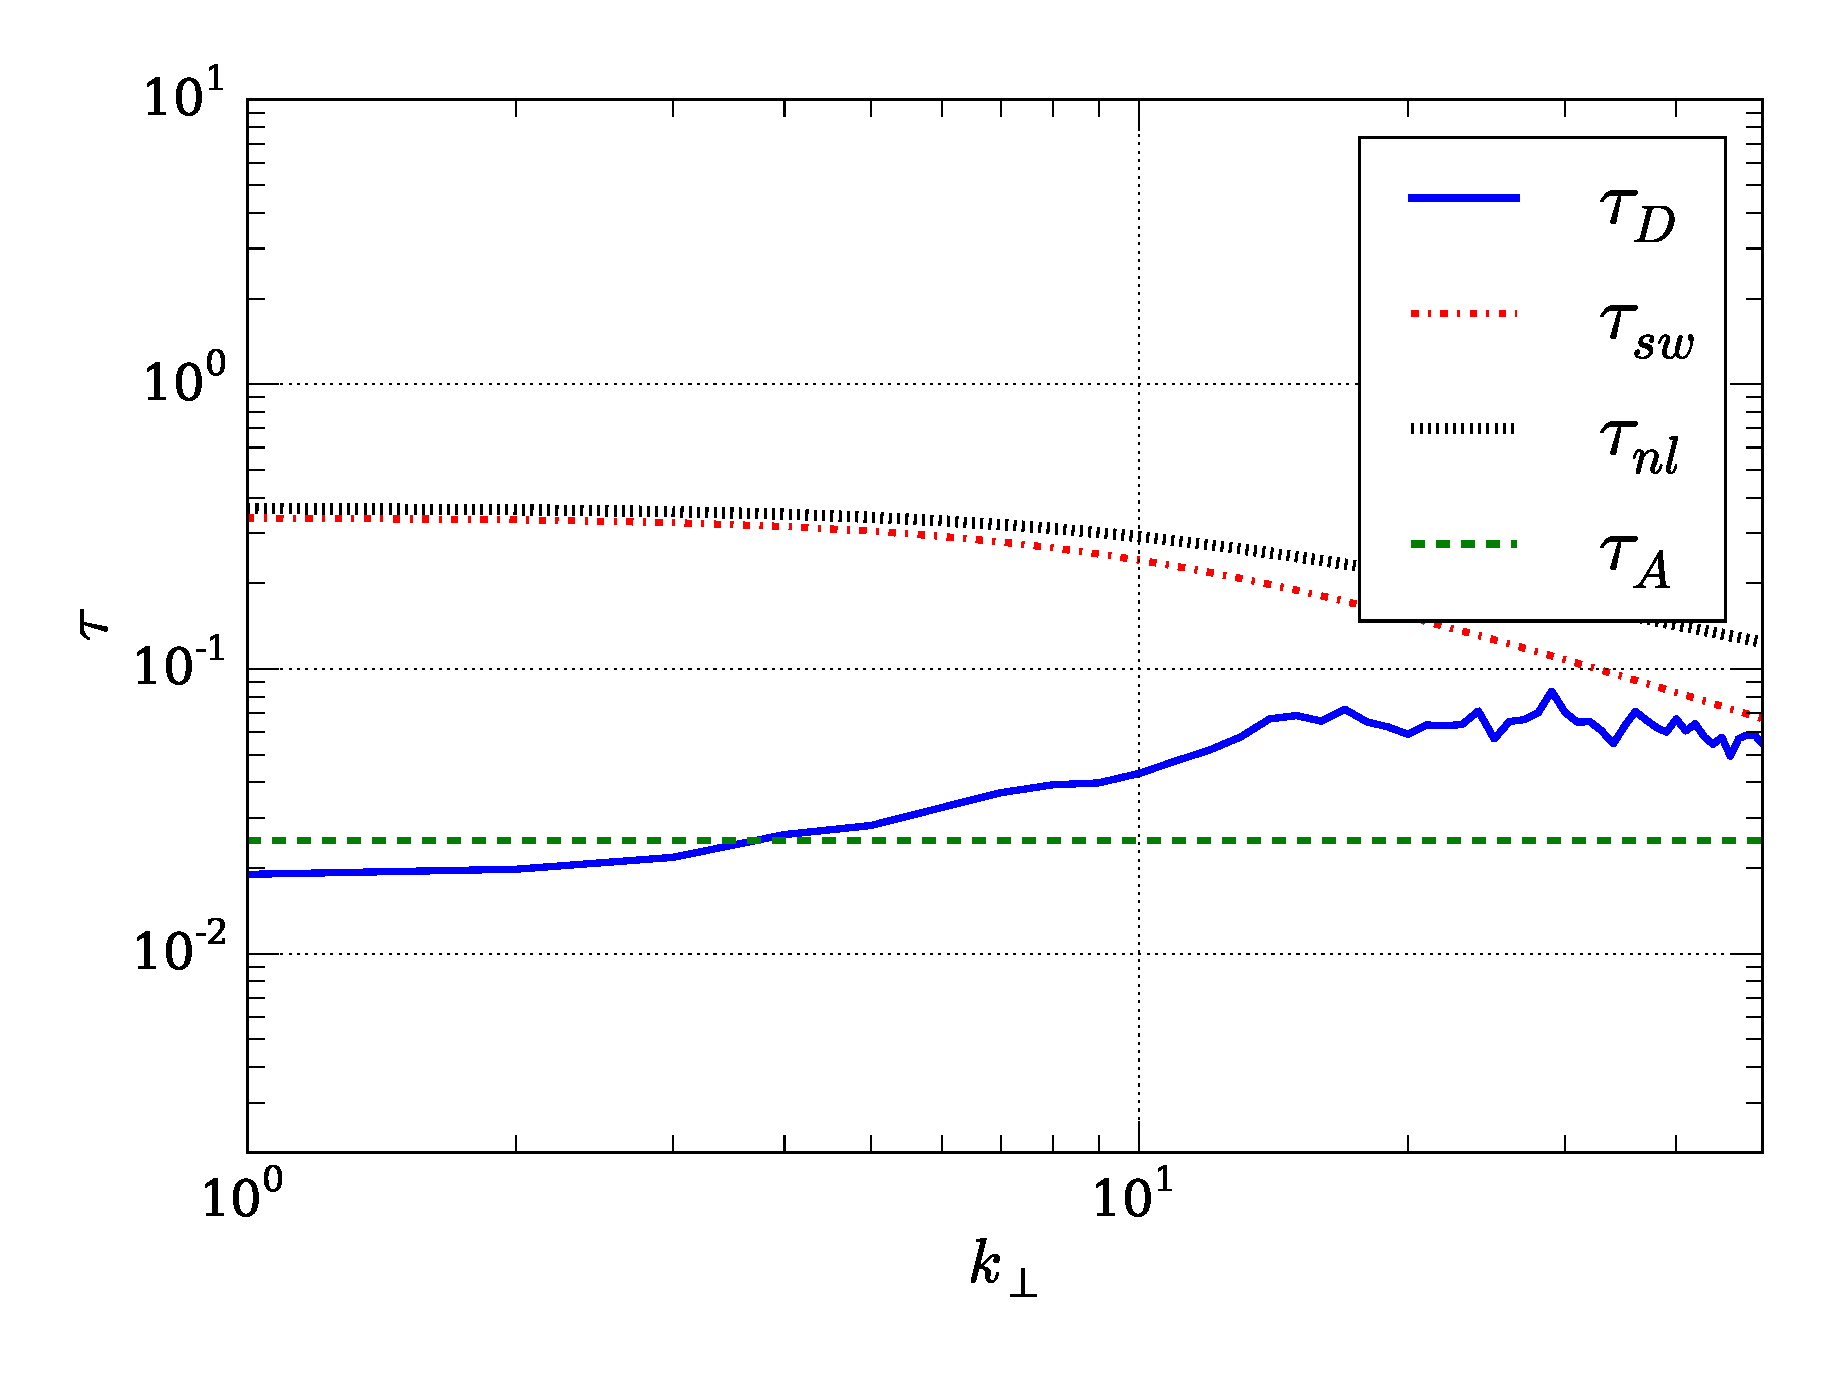
\includegraphics[width=0.76\columnwidth]{P1/fig5_B8_b_kpara_10.eps}
      \end{center}
    \end{minipage}
  \end{columns}
  \vspace{-0.5cm}
  \begin{center}
    $k_\parallel = 20$\\
    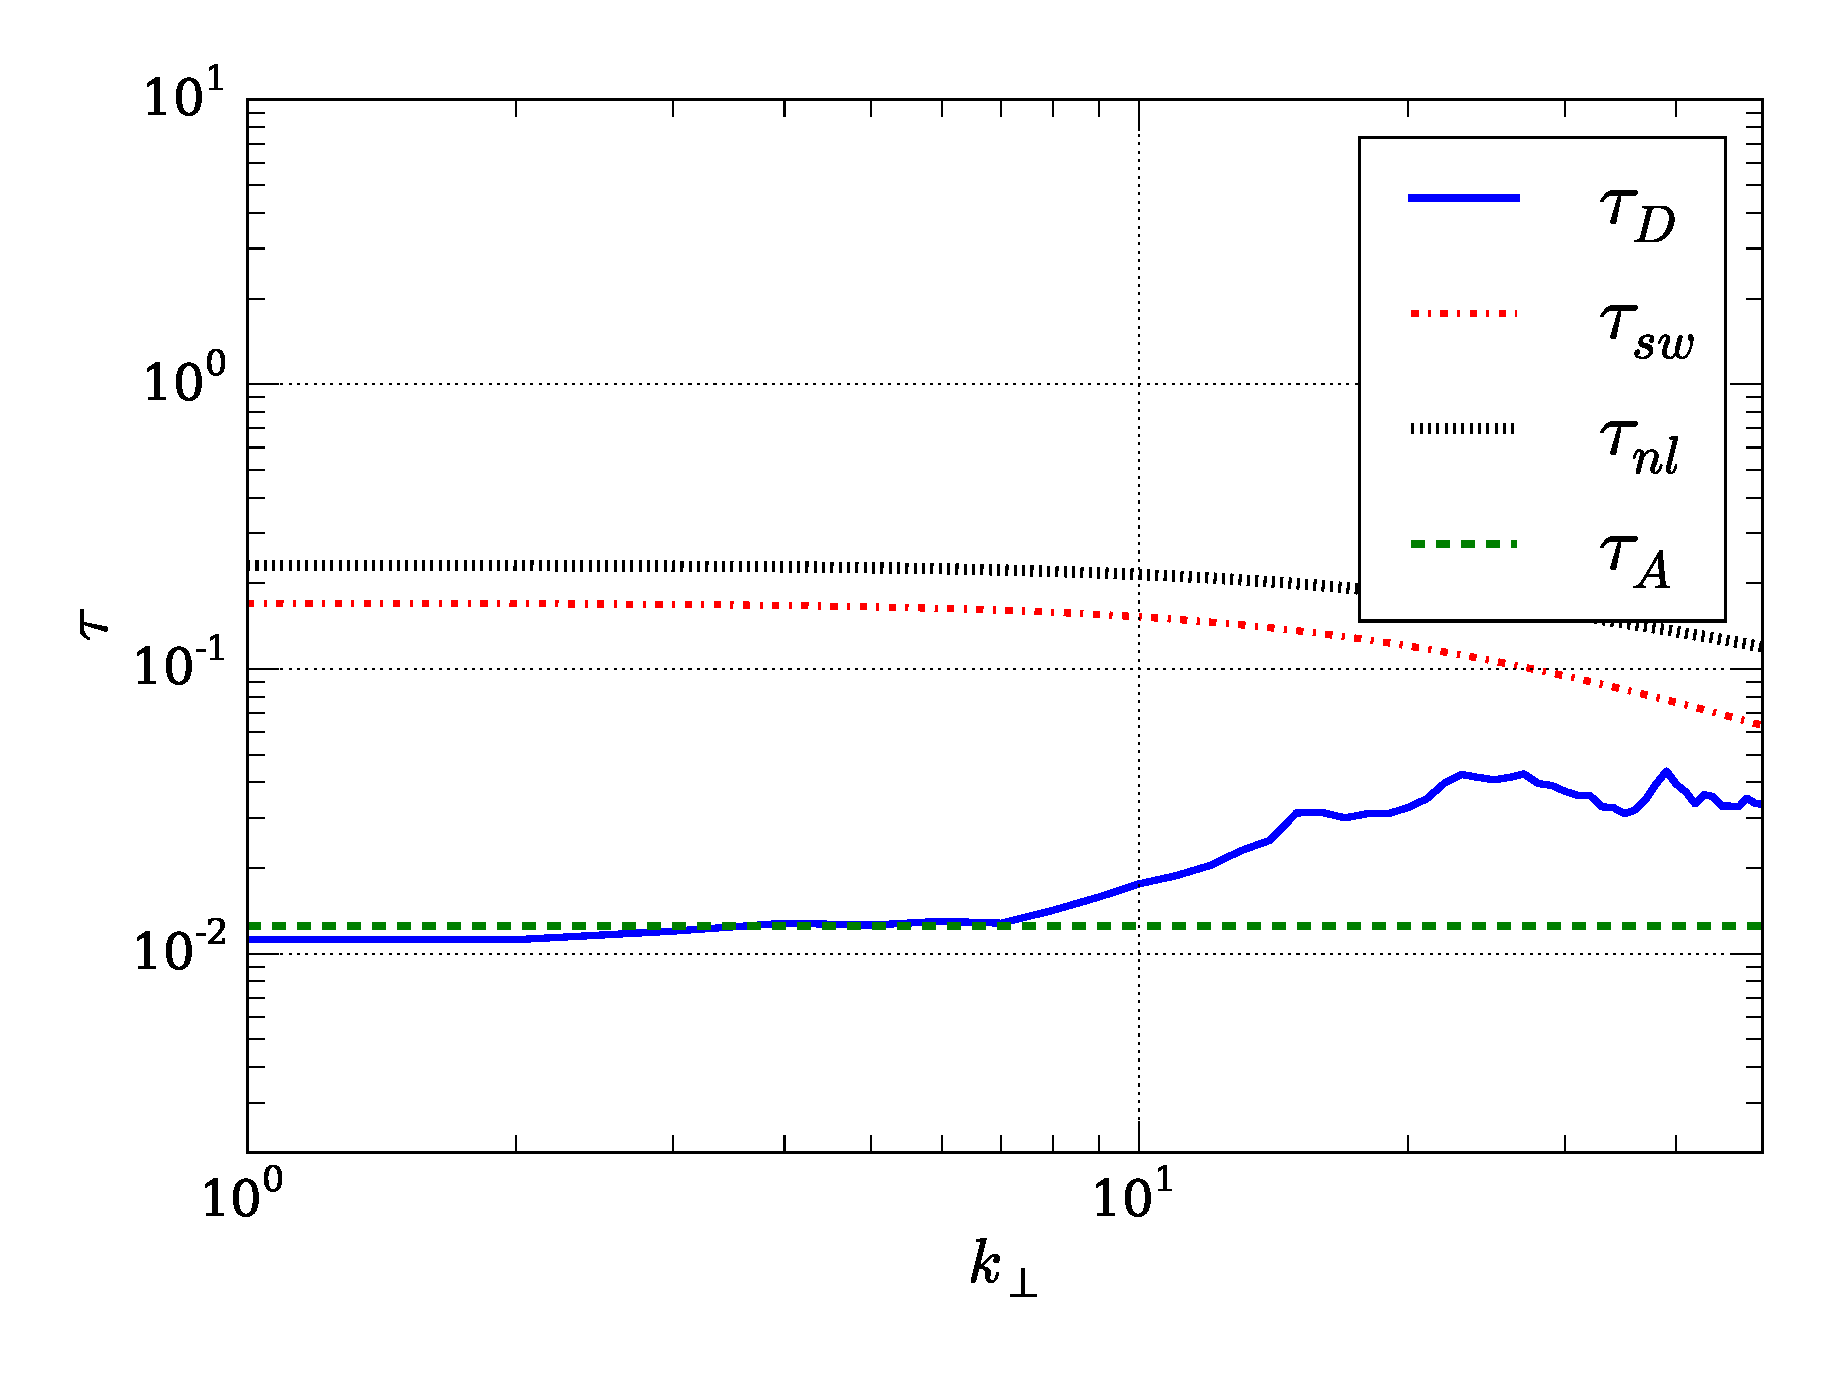
\includegraphics[width=0.38\columnwidth]{P1/fig5_B8_b_kpara_20.eps} \\
  \end{center}
}
\note[itemize]{
\item Para valores pequeños de $k_\perp$, el tiempo de Alfvén
  domina. Después, $\tau_D$ se acerca al \emph{sweeping}.
}


%\section{Conclusions}
\frame{\frametitle{Conclusiones hasta aquí...}
\pause
  \begin{itemize}
  \item Los efectos no locales (en el espacio espectral) juegan un rol
    importante en la turbulencia MHD y la descorrelación se encuentra
    principalmente dominada por el \emph{sweeping} y las interacciones
    Alfv\'enicas.
  \item El análisis presentado aquí permite \textbf{distinguir entre esos dos
    efectos}: las interacciones de \emph{sweeping} dominan la
    descorrelación para valores moderados de $B_0$, mientras que para
    grandes valores del campo medio $B_0$ y a grandes escalas las
    descorrelaciones están controladas mayoritariamente por las
    interacciones Alfv\'enicas.
  \item \textbf{El sistema elige el
    tiempo de descorrelación más corto disponible}. Aún
    para grandes valores del campo guía $B_0$, para escalas
    suficientemente pequeñas en las que el tiempo de \emph{sweeping}
    se vuelve más rápido que el tiempo de Alfv\'en, luego de un amplio
    rango de escalas dominadas por las ondas de Alfv\'en, el sistema
    transiciona hacia un comportamiento dominado por el
    \emph{sweeping}.
  \end{itemize}
}
\note[itemize]{
\item 2) SW+Alfvén confirma Servidio.
\item 3) Un constructo simple y relevante es que la tasa de
  descorrelación es la suman de las tasas asociadas con cada escala de
  tiempo relevante.
}


\frame{\frametitle{Conclusiones hasta aquí...}
  \begin{itemize}
  \item Extrapolación difícil de las conclusiones para aplicaciones
    espaciales y astrofísicas, pero sí resultados cualitativos.
  \item En MHD, tanto el \emph{sweeping} como la propagación de ondas
    de Alfv\'en contribuyen a la variación de tiempo total en un punto
    (espectro Euleriano en frecuencias), y por lo tanto influyen en
    una predicción limitante.
  \end{itemize}
}
\note[itemize]{
\item Por ejemplo, el viento solar admite $\delta B/B_0 \sim
    1$ en la escala más externa. Aún si el cociente es menor, por
    ejemplo a escalas menores en el rango inercial, el presente
    resultado sugiere que \textbf{el efecto de \textit{sweeping} se mantendría
    importante en establecer la tasa del tiempo de descorrelación en
    el ambiente interplanetario}.
\item
\item HELICIDAD CRUZADA
\item Para estudiar teniendo en cuenta el sentido de las propagaciónes, variables de Elsässer. Ahora el sentido de las propagaciones nos importa.

}





\frame{\frametitle{Variando la helicidad cruzada: Campos de Els\"asser}
  Las ecuaciones MHD en función de los campos de Els\"asser:
  \begin{equation*}\label{eq:ElsasserFields}
    \vec{z}^\pm = \vec{v} \pm \vec{b}
  \end{equation*}
  \begin{equation*}\label{eq:NS-Elsasser}
    \partial_t \vec{z}^\pm  = \pm  \vec{V_A} \cdot \nabla \vec{z}^\pm  - 
    \vec{z}^\mp \cdot \nabla \vec{z}^\pm - \nabla{P} + 
    \frac{1}{R} \nabla^2 \vec{z}^\pm
  \end{equation*}

  \begin{itemize}
    \item Asumimos: $P = p/\rho$ y $R = R_m$
  \end{itemize}
  \pause\vspace{10pt}
  \begin{columns}
    \column{0.8\textwidth}
    \begin{minipage}[t]{1\textwidth}
      \begin{center} 
  Invariantes ideales de MHD incompresible:
  \begin{equation*}
    E = \frac{1}{2}\int{\left(\left|\vec{v}\right|^2 +
      \left|\vec{b}\right|^2 \right)\,dV} =
    \frac{1}{4}\int{\left(\left|\vec{z}^+\right|^2 +
      \left|\vec{z}^-\right|^2 \right)\,dV}
  \end{equation*}
  \begin{equation*}
    H_c = \int{\vec{v}\cdot\vec{b} \, dV} =
    \frac{1}{4}\int{\left(\left|\vec{z}^+\right|^2 
    - \left|\vec{z}^-\right|^2 \right)\,dV}
  \end{equation*}
      \end{center}
    \end{minipage}
    \column{0.2\textwidth}
    \begin{minipage}[t]{1\textwidth}
      \begin{center}
        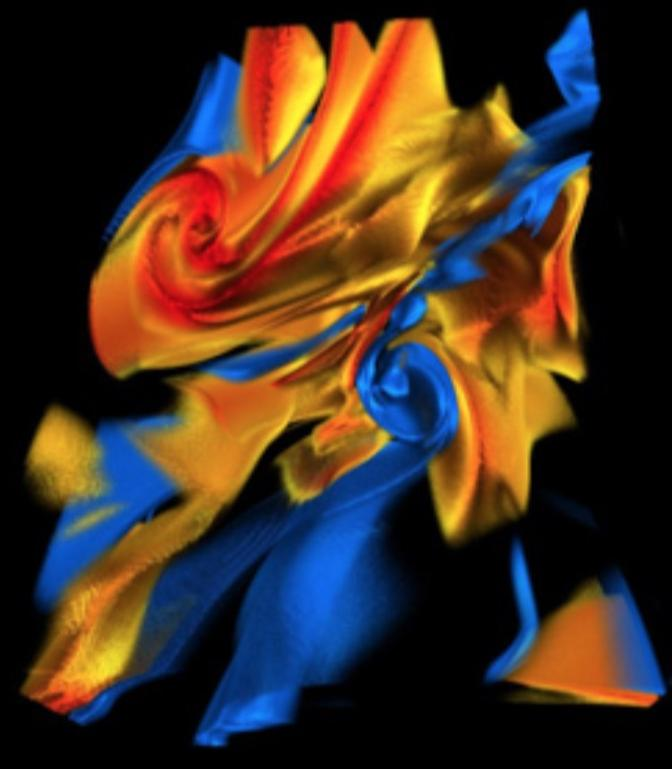
\includegraphics[width=\columnwidth]{extra/helicidad1.jpg}
      \end{center}
    \end{minipage}
  \end{columns}

}
\note[itemize]{
\item Para estudiar teniendo en cuenta el sentido de las propagaciónes, variables de Elsässer. Ahora el sentido de las propagaciones nos importa.
  \item Campos de las perturbaciones.
  \item Miembro derecho: térmico convectivo separado en parte lineal
    (propagación Alfvénica con $\vec{V_A}=\vec{B_0}$) y parte no
    lineal (interacción de fluctuaciones contrapropagantes).
  \item La helicidad cruzada es de relevancia para el viento solar y
    para los plasmas espaciales, pues los flujos de gran escala con
    helicidad cruzada se encuentran usualmente en el medio
    interplanetario.
}



\frame{\frametitle{Campos de Els\"asser}
  \begin{equation*}
    H_c = \int{\vec{v}\cdot\vec{b} \, dV} =
    \frac{1}{4}\int{\left(\left|\vec{z}^+\right|^2 
    - \left|\vec{z}^-\right|^2 \right)\,dV}
  \end{equation*}
  Podemos definir la helicidad cruzada normalizada:
  \begin{equation*}
    \sigma_c = H_c/E
  \end{equation*}
  \vspace{-20pt}
  \begin{itemize}
    \item $\sigma_c$ mide la cantidad de fluctuaciones
      contrapropagantes en el sistema.
    \item $\sigma_c = \pm 1$ corresponde a un único tipo de
      fluctuaciones $\vec{z}^\pm$, mientras $\sigma_c=0$ representa
      equipartición entre ambos campos.
    \item El estudio espacio-temporal de las variables de Els\"asser
      nos permitirá separar las dos posibles polarizaciones de las
      ondas de Alfvén, así como también las direcciones de
      propagación, y cuantificar cualquier desbalance entre ellas.
  \end{itemize}
}
\note[itemize]{
  \item
  \item SIMULACIONES
}




\frame{\frametitle{Simulaciones realizadas}
  \begin{table}
    \centering
    \begin{tabular}{|l||c||c||c||c||c||c|}
      \hline
      & $B_0=0$ & $B_0 = 0.25$ & $B_0 = 1$ & $B_0 = 2$ & $B_0 = 4$ & $B_0 = 8$ \\ \hline\hline
      & $0$ & $0$ & $0$ & $0$ & $0$ & $0$ \\ \cline{2-7} 
      $\sigma_c \approx $ & $0.3$ & $0.3$ & $0.3$ & $0.3$ & $0.3$ & $0.3$ \\ \cline{2-7} 
      & $0.9$ & $0.9$ & $0.9$ & $0.9$ & $0.9$ & $0.9$ \\ \hline
    \end{tabular}
    %\caption{Lista de simulaciones numéricas realizadas, con un campo guía
    %  $\vec{B} = B_0 \hat{x}$ y helicidad cruzada normalizada $\sigma_c$.}
    \label{tab:listSim}
  \end{table}
  \begin{itemize}
    \item Correlaciones entre los forzados mecánico y magnético para
      cambiar el nivel de helicidad cruzada en el flujo.
    \item Los $\sigma_c$ corresponden al promedio temporal en el estado
      turbulento estacionario.
    \item Todas las simulaciones fueron realizadas hasta que el
      sistema alcanzase un estado turbulento estacionario.
  \end{itemize}
}
\note[itemize]{
  \item Cada simulación tiene una helicidad cruzada instantánea que
    fluctúa en el tiempo alrededor de los valores medios reportados.
}







\frame{\frametitle{Espectros de energía y escalas de tiempo dominantes}
  Los espectros energéticos perpendiculares reducidos y los
  isocontornos del espectro axisimétrico de energía son similares a
  los ya obtenidos.
  \begin{columns}
    \column{0.4\textwidth}
    \begin{minipage}[t]{1\textwidth}
      \begin{center} 
        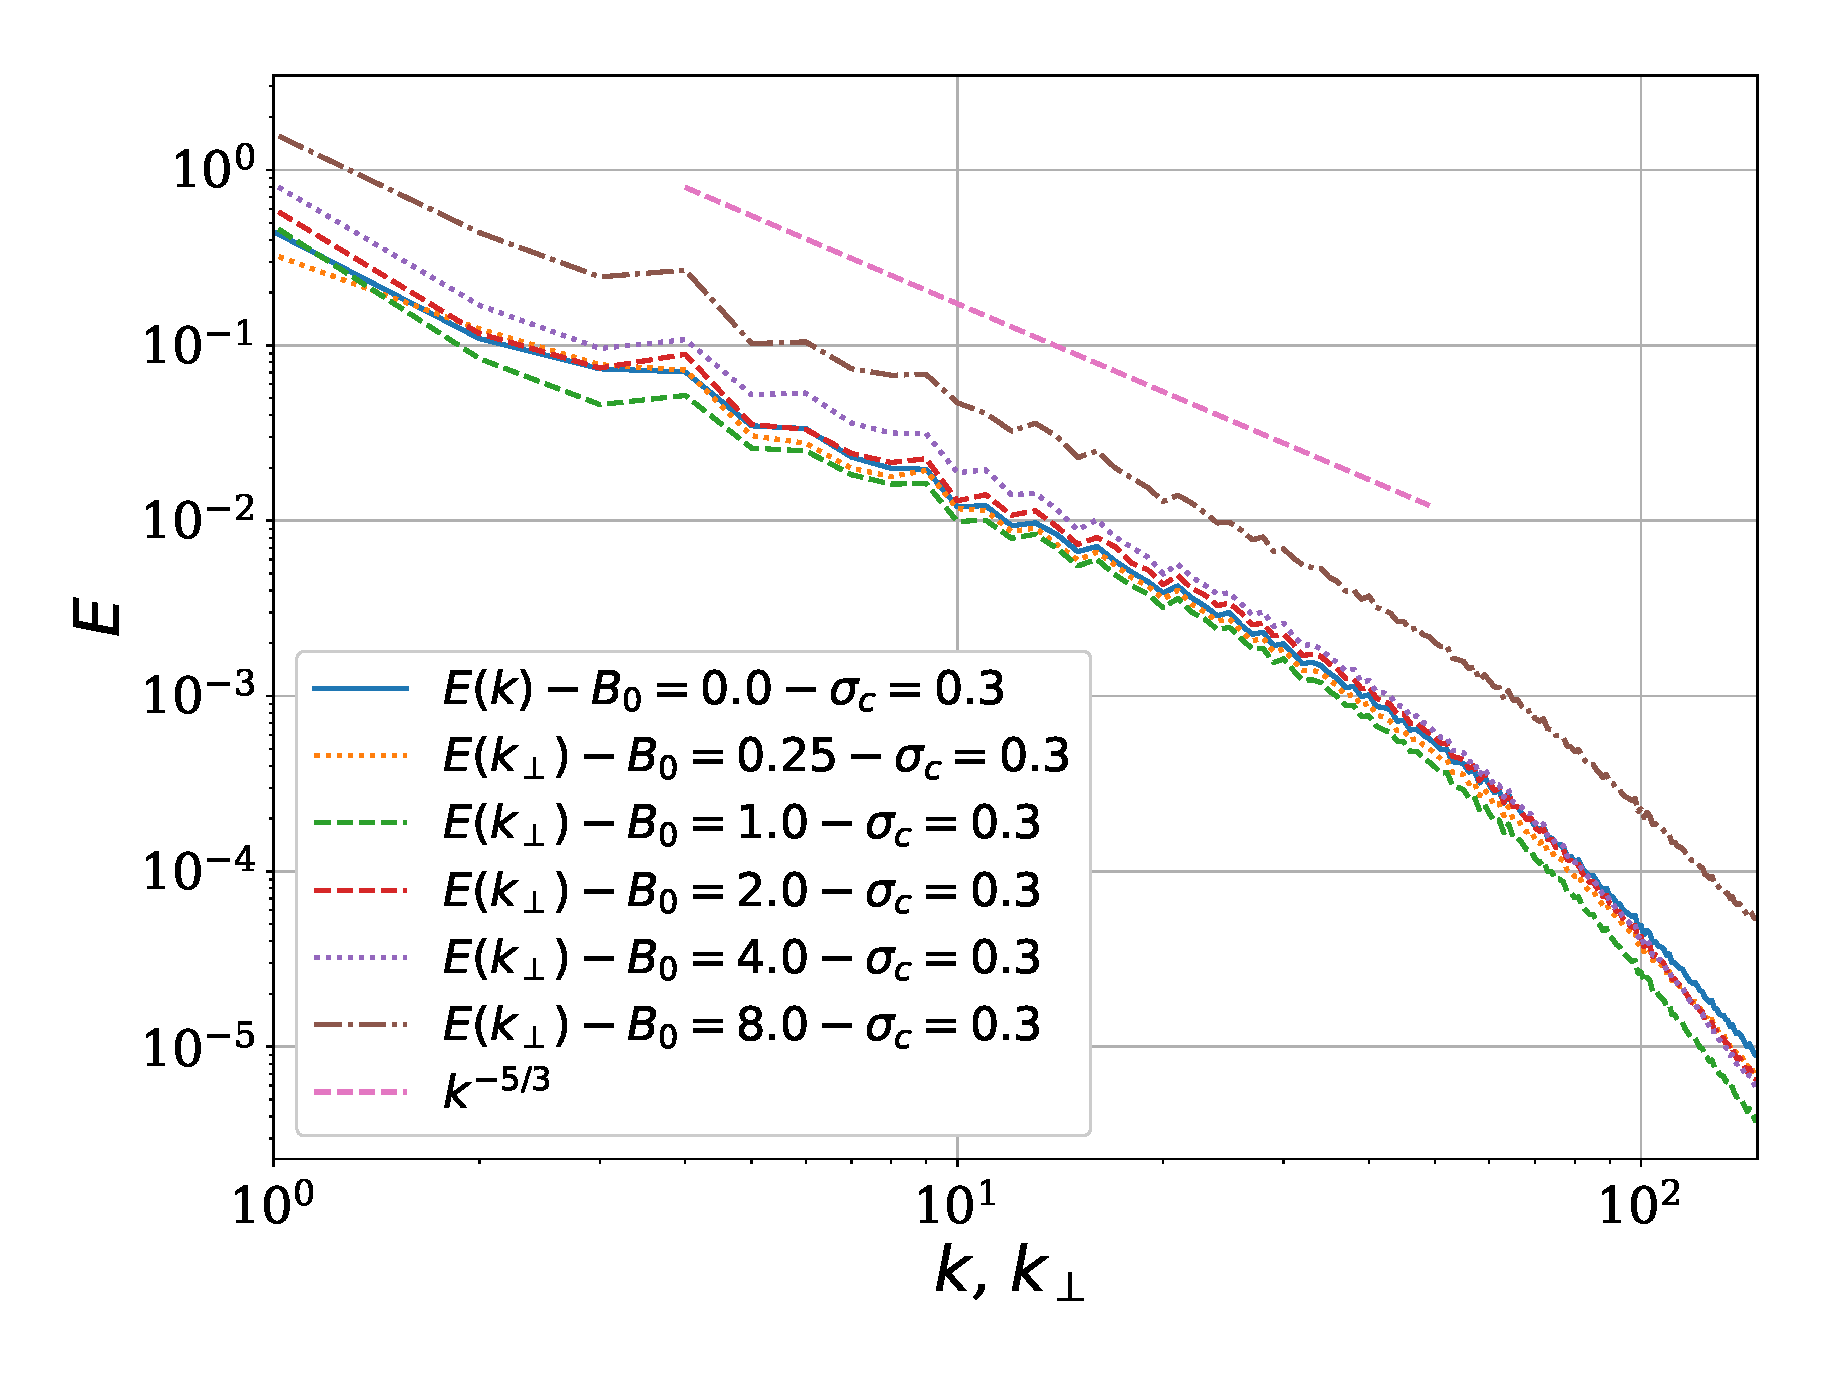
\includegraphics[width=\columnwidth]{P2/fig1_E.eps}
      \end{center}
    \end{minipage}
    \column{0.3\textwidth}
    \begin{minipage}[t]{1\textwidth}
      \begin{center}
        {\large $B_0 = 0$}\\
        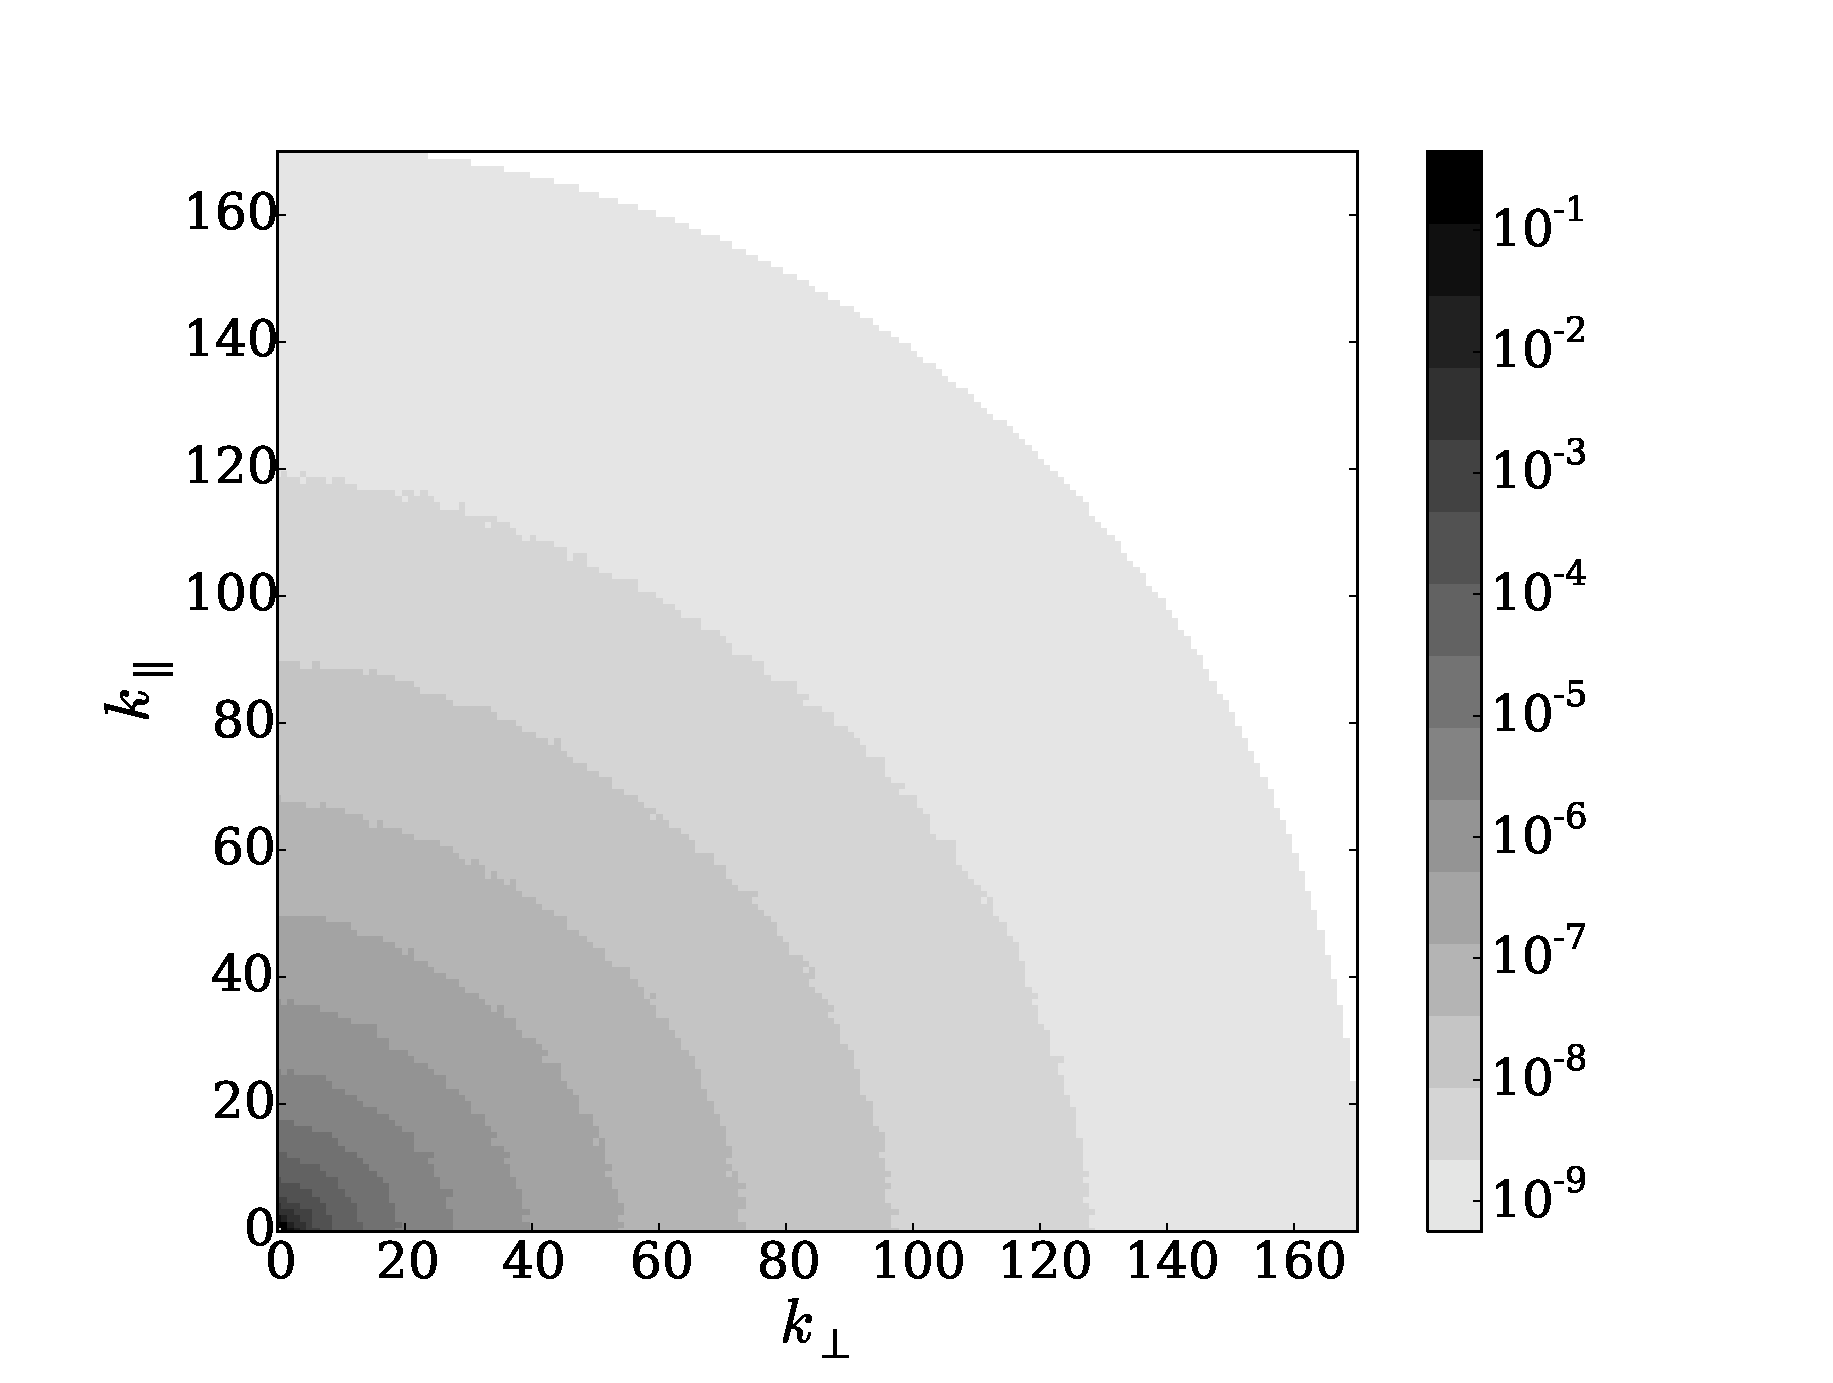
\includegraphics[width=\columnwidth]{P1/fig2_B0.eps} \\
        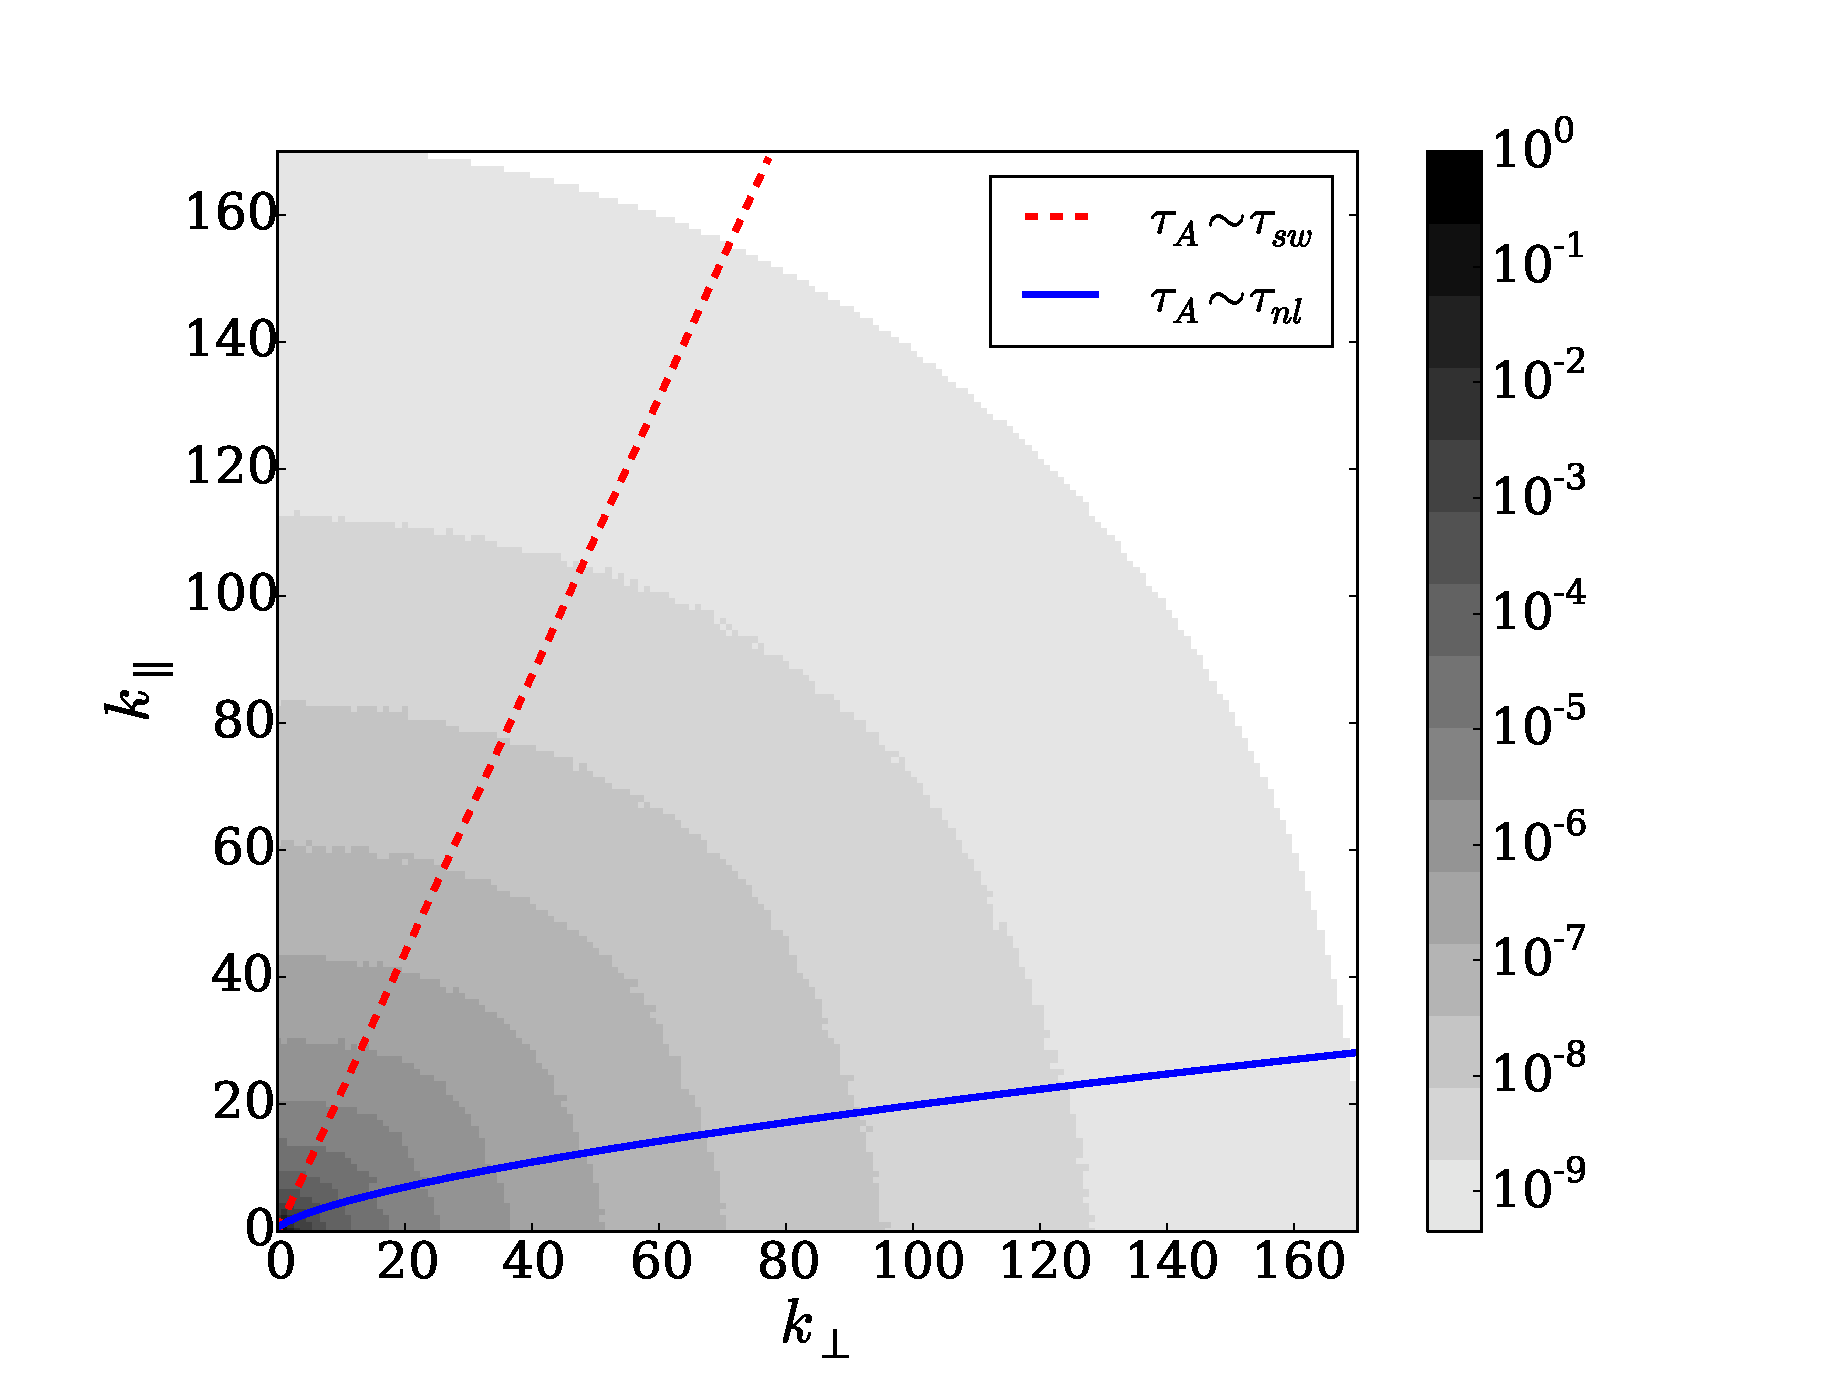
\includegraphics[width=\columnwidth]{P1/fig2_B1.eps} \\
        {\large $B_0 = 1$}
      \end{center}
    \end{minipage}
    \column{0.3\textwidth}
    \begin{minipage}[t]{1\textwidth}
      \begin{center}
        {\large $B_0 = 4$}\\
        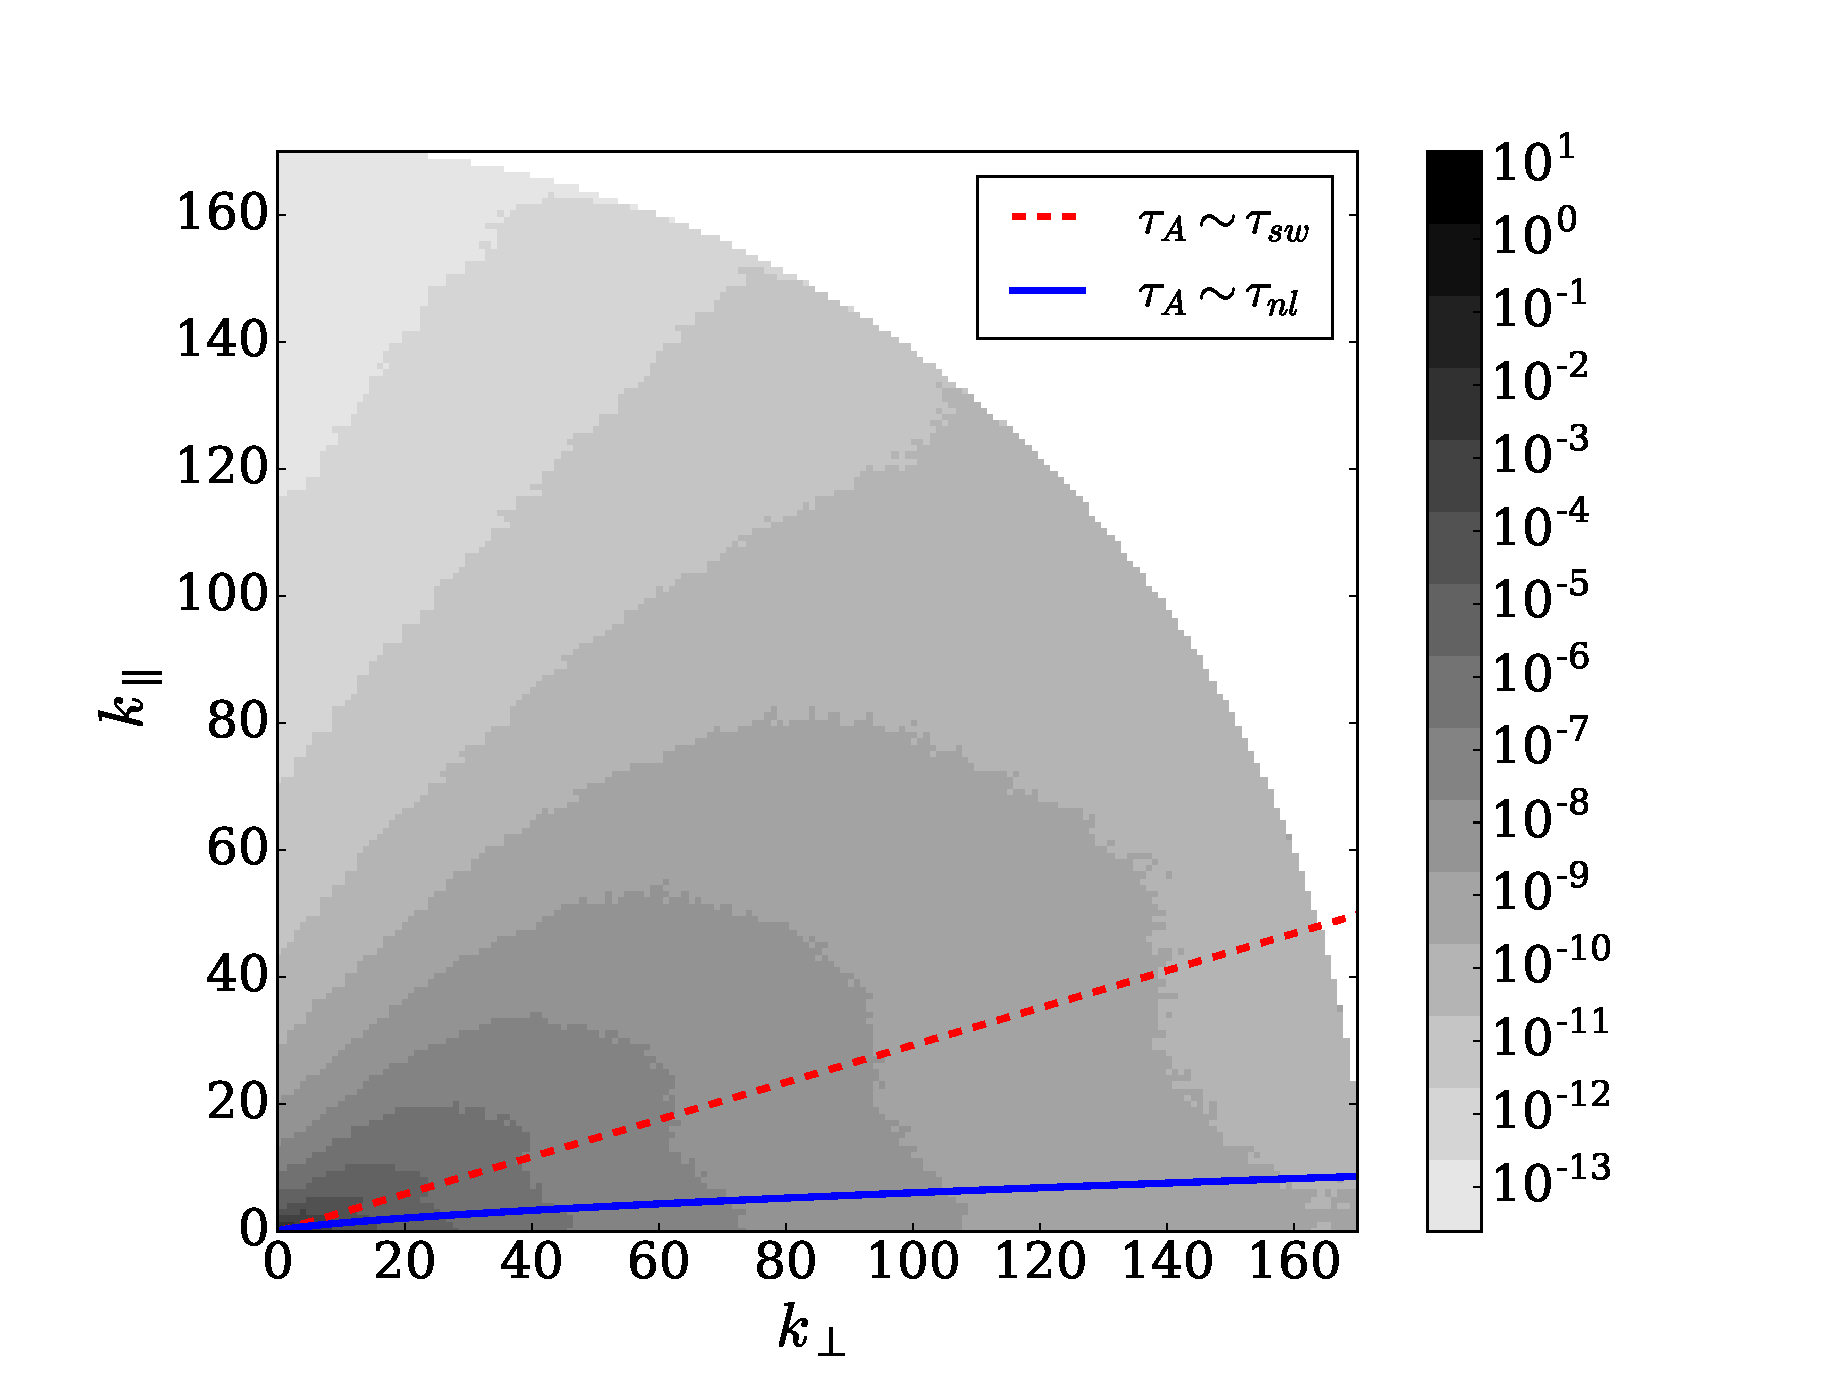
\includegraphics[width=\columnwidth]{P1/fig2_B4.eps} \\
        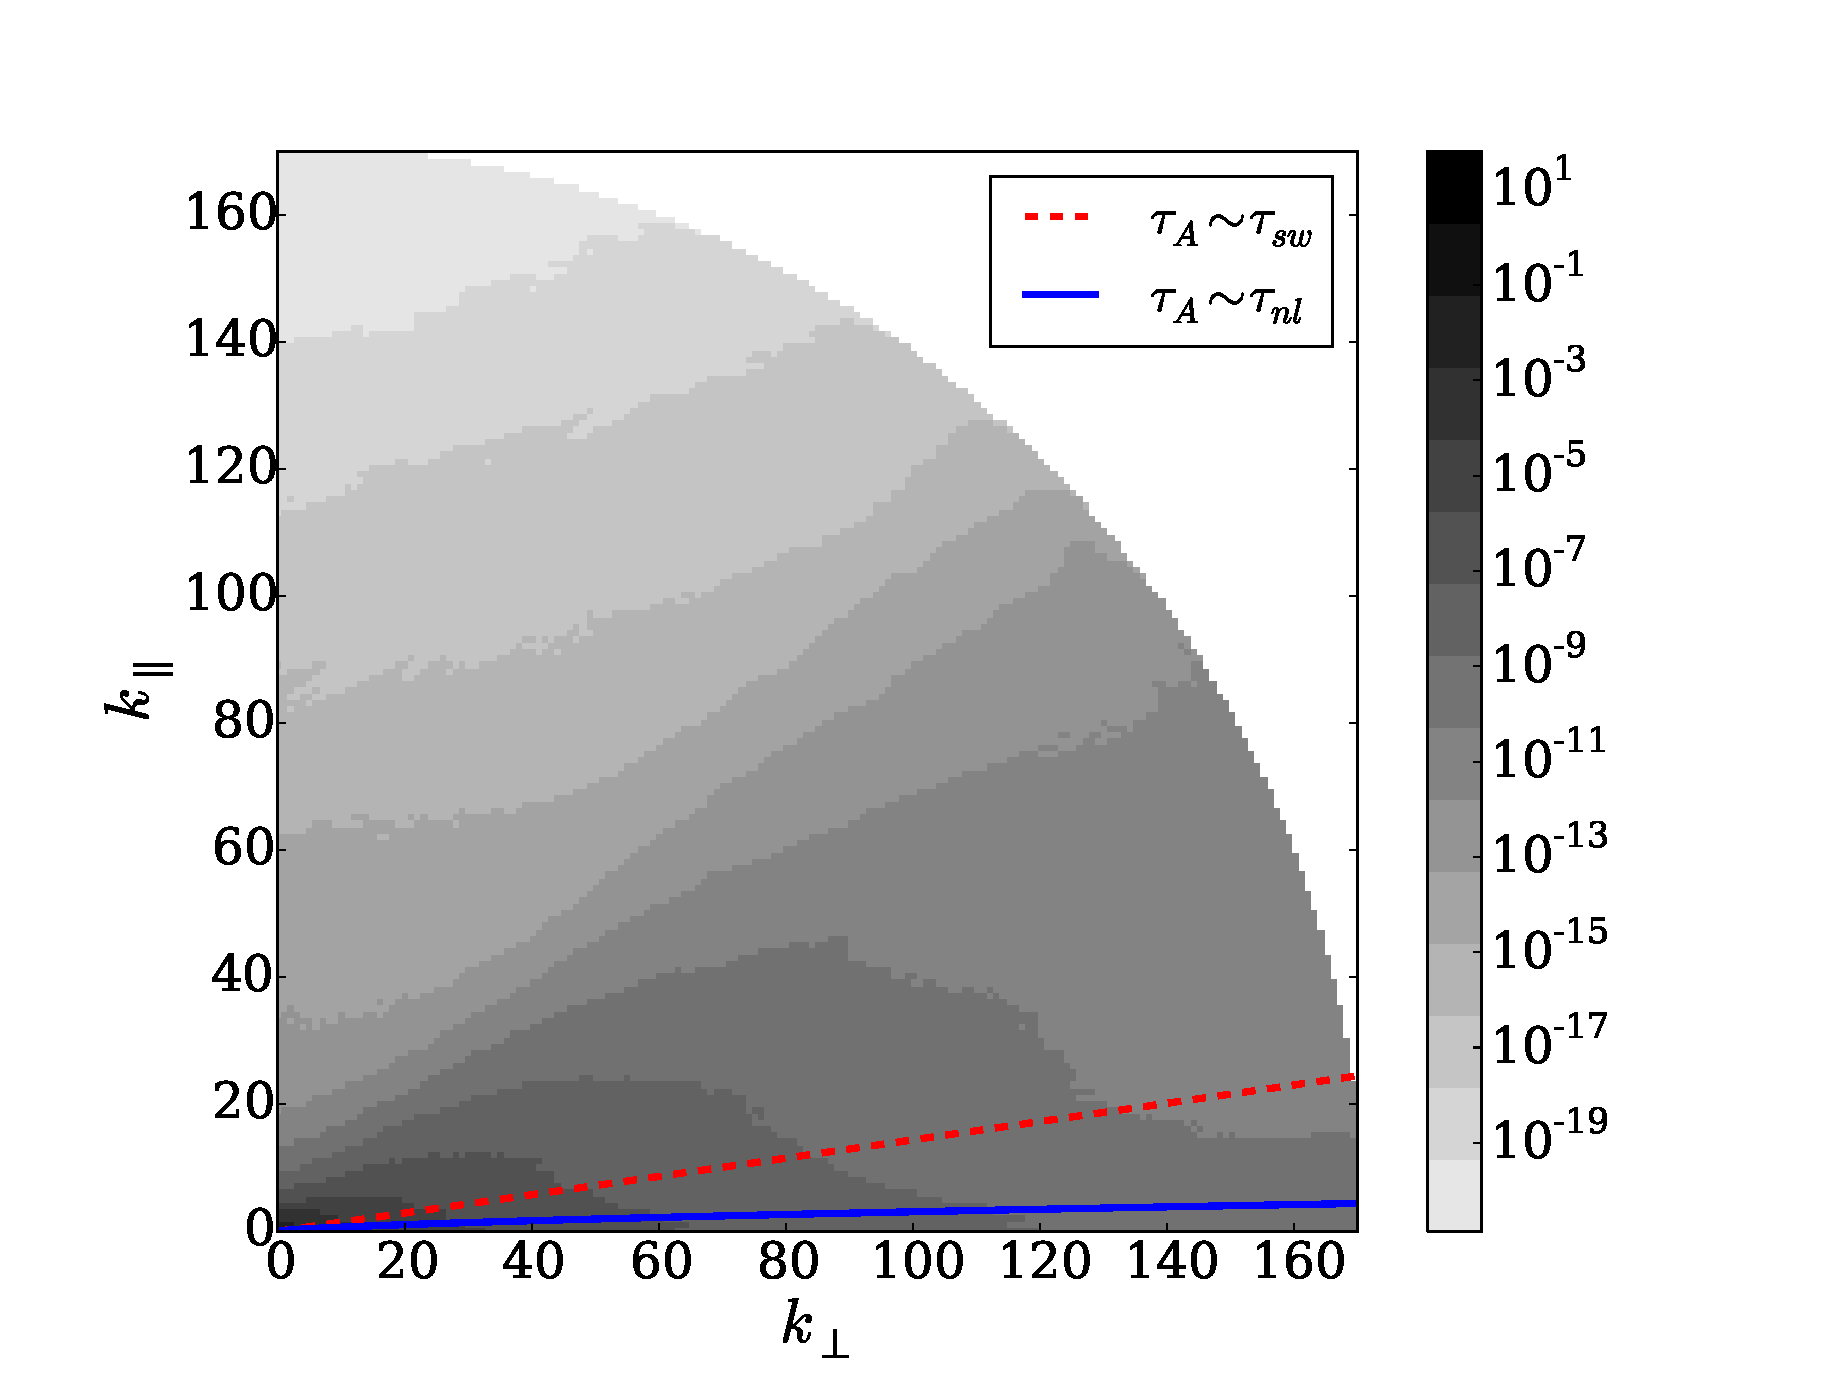
\includegraphics[width=\columnwidth]{P1/fig2_B8.eps} \\
        {\large $B_0 = 8$}
      \end{center}
    \end{minipage}
  \end{columns}
}
\note[itemize]{
  \item Los isocontornos cambian de
    forma a medida que cruzan cada una de estas líneas para $B_0$ grande.
  \item Aumento de anisotropía a medida que $B_0$ se incrementa, así
    como también la mayor superficie cubierta por modos en los que el
    período de Alfv\'en es el tiempo más rápido.  }




\frame{\frametitle{Espectros espacio-temporales}
}
\note[itemize]{
\item Acá están los principales resultados.
\item Espectro normalizado, con $k_\perp=0$ y en función de
  $k_\parallel$ y $\omega$.
}






\frame{\frametitle{Espectros espacio-temporales}
  {\large \underline{Espectro energético normalizado $E({\bf k}, \omega)/E({\bf k})$}}
  {\large, $B_0 = 0$}\vspace{10pt}
  \begin{columns}
    \column{0.5\textwidth}
    \begin{minipage}[t]{1\textwidth}
      \begin{center}
        {$\vec{z}^-$, $\sigma_c = 0.3$} \\
        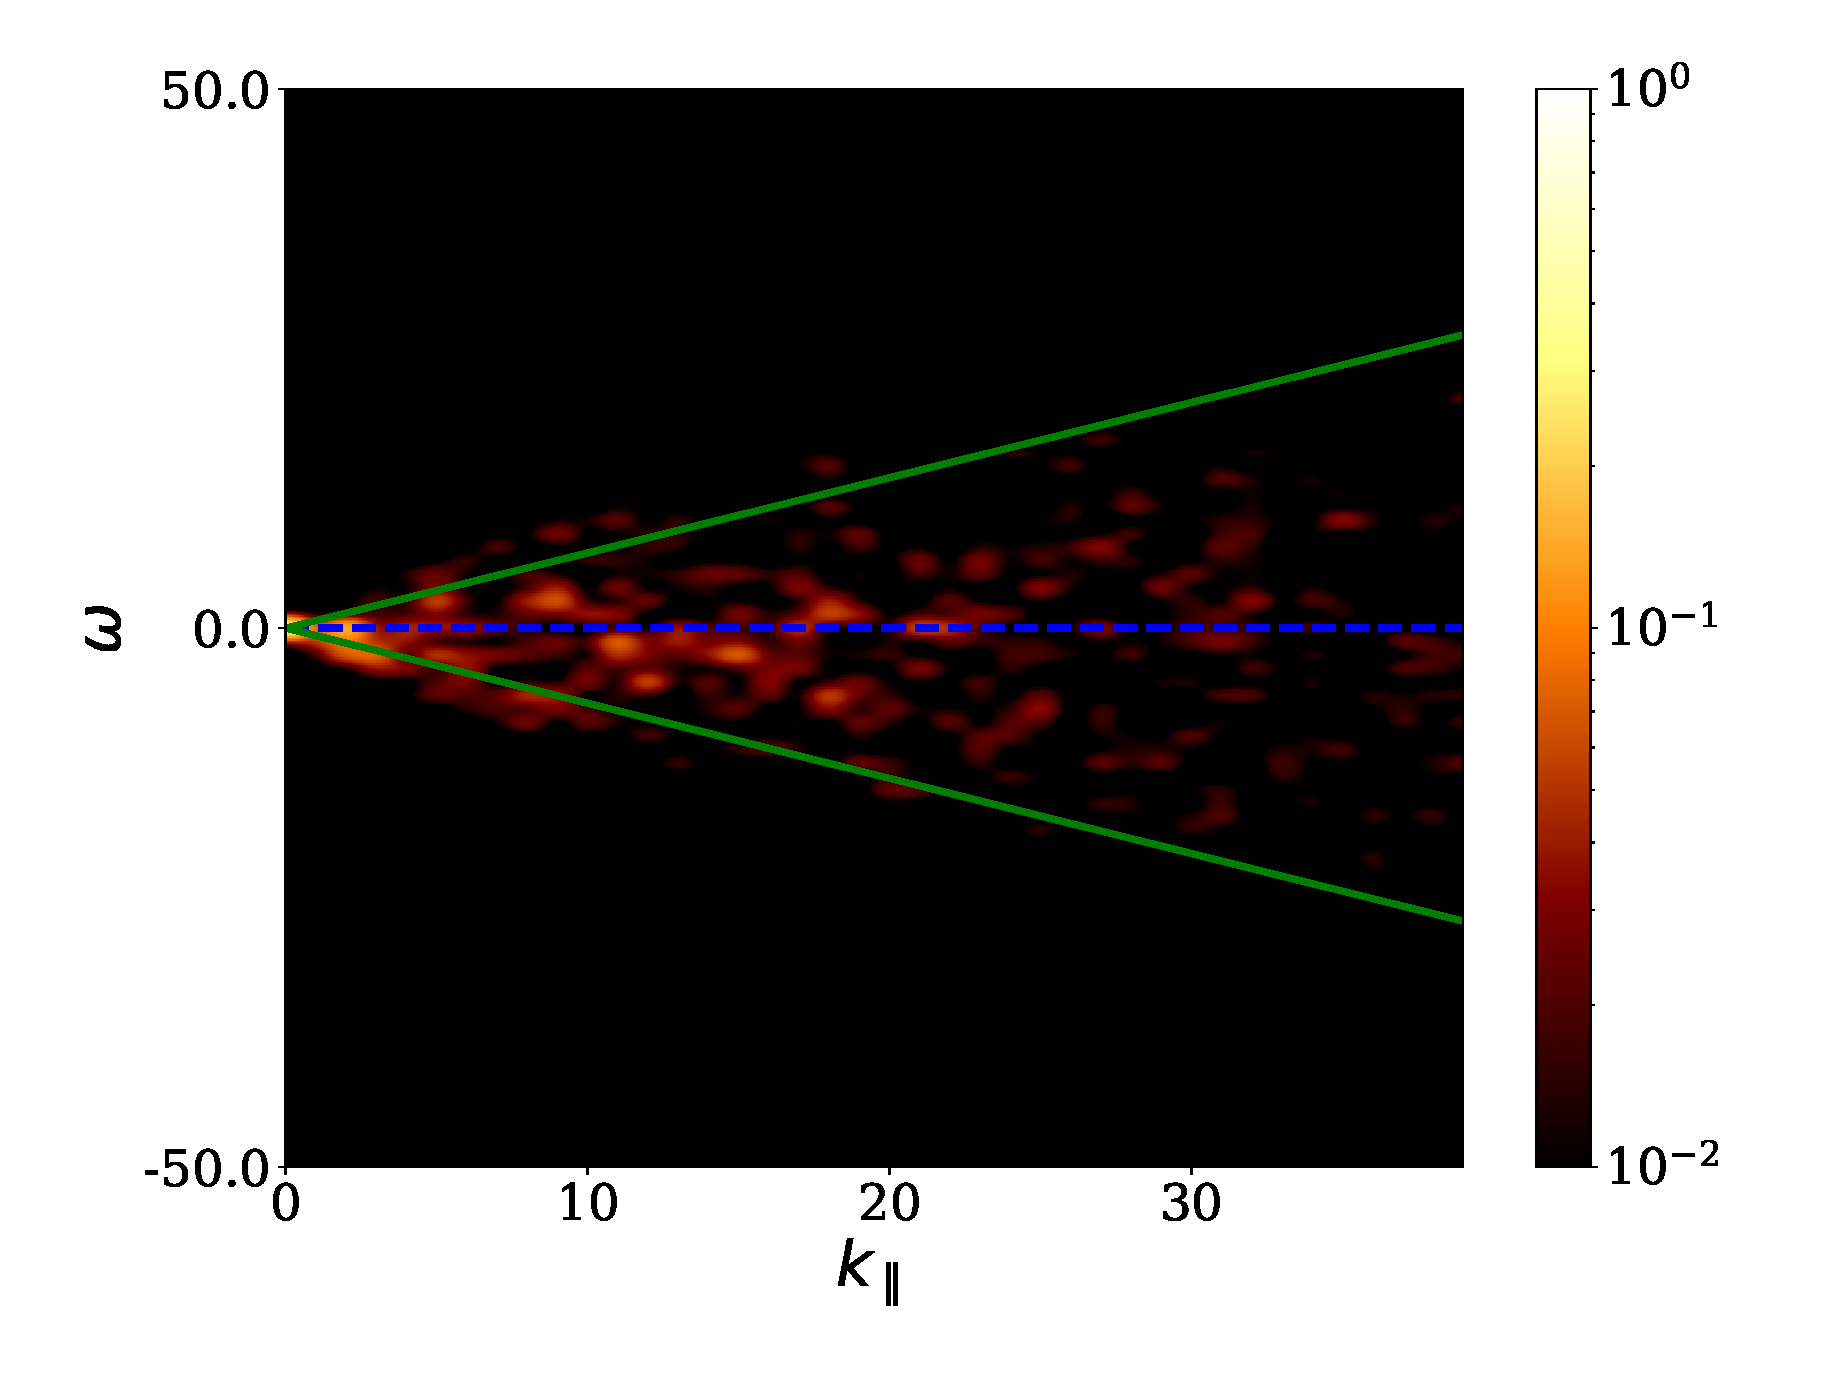
\includegraphics[width=0.65\textwidth]{{P2/fig3_B0.0_y_Hc0.3_zm_kperp0}.eps} \\
        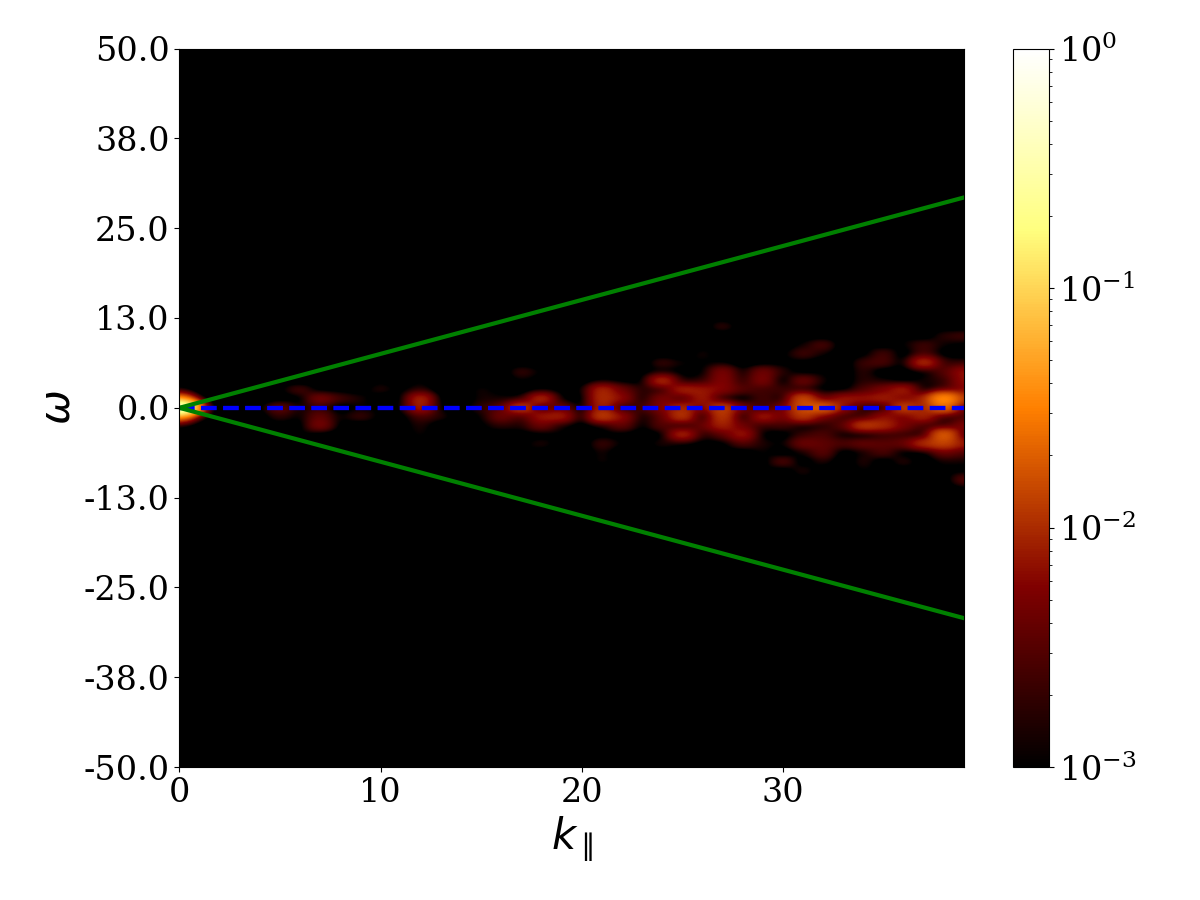
\includegraphics[width=0.65\textwidth]{{P2/fig3_B0.0_y_Hc0.9_zm_kperp0}.eps} \\
        {$\vec{z}^-$, $\sigma_c = 0.9$}
      \end{center}
    \end{minipage}
    \column{0.5\textwidth}
    \begin{minipage}[t]{1\textwidth}
      \begin{center}
        {$\vec{z}^+$, $\sigma_c = 0.3$} \\
        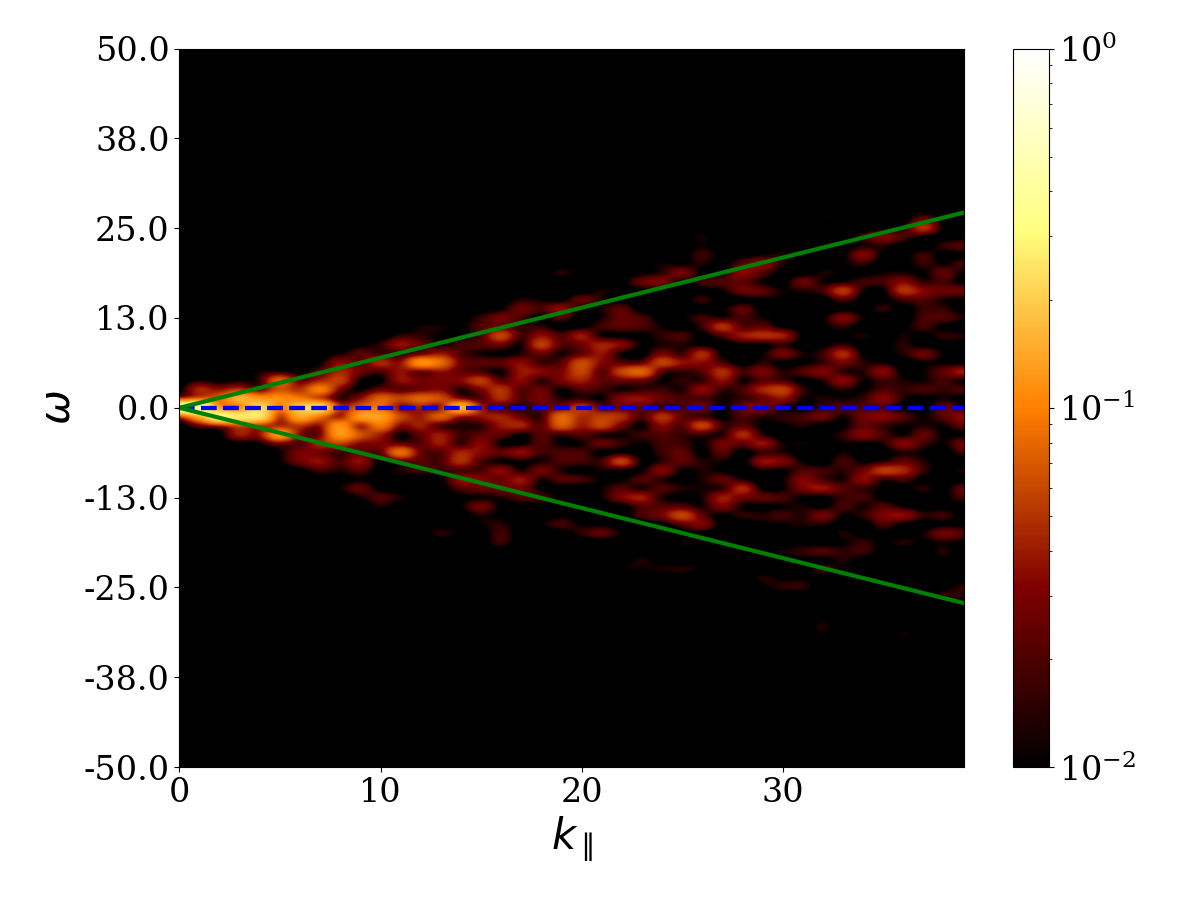
\includegraphics[width=0.65\textwidth]{{P2/fig3_B0.0_y_Hc0.3_zp_kperp0}.eps} \\
        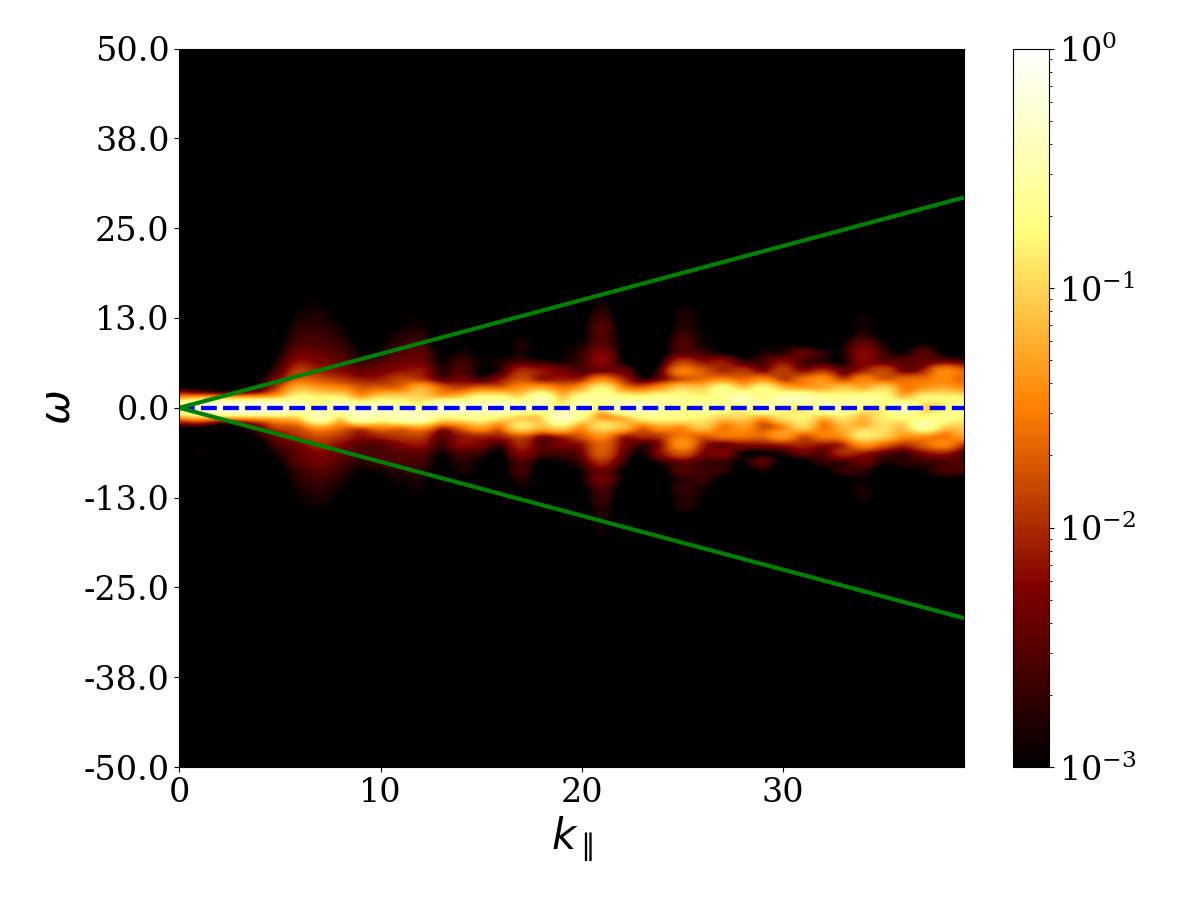
\includegraphics[width=0.65\textwidth]{{P2/fig3_B0.0_y_Hc0.9_zp_kperp0}.eps} \\
        {$\vec{z}^+$, $\sigma_c = 0.9$}
      \end{center}
    \end{minipage}
  \end{columns}
}
\note[itemize]{
\item $k_\perp=0$ fijo. Líneas de \emph{sweeping} y Alfvén.
\item Espectro: Fourier en $t$ y $r$ de $\vec{z}^\pm$. Acumulación de
  energía.
\item Alfvén ($\omega=0$) indistinguible de los modos lentos (ej, \textit{eddies}).
\item E en todo el embudo, evidenciando turbulencia fuerte
  en todas las escalas, más que turbulencia de ondas o propagación
  lineal de ondas.
\item Para $\sigma_c$ grande, energía en $\omega\approx 0$ y en
  $\vec{z}^+$.
\item Para $B_0=0$ y $\sigma_c=0$, la escala de tiempo dominante es la
  del \textit{sweeping}, mientras que para grandes valores de
  $\sigma_c$, se vuelven dominantes o bien la escala temporal no
  lineal o el tiempo de Alfvén.
\item Mayor $\sigma_c$, más E en $\vec{z}^+$.
}



\frame{\frametitle{Espectros espacio-temporales}
  {\large \underline{Espectro energético normalizado $E({\bf k}, \omega)/E({\bf k})$}}
  {\large, $B_0 = 1$}\vspace{10pt}
  \begin{columns}
    \column{0.33\textwidth}
    \begin{minipage}[t]{1\textwidth}
      \begin{center}
        {$\vec{z}^+$, $\sigma_c = 0.0$} \\
        \includegraphics[width=0.95\textwidth]{{P2/fig3_B1.0_y_Hc0.0_zp_kperp0}.eps} \\
        \includegraphics[width=0.95\textwidth]{{P2/fig3_B1.0_y_Hc0.0_zm_kperp0}.eps} \\
        {$\vec{z}^-$, $\sigma_c = 0.0$}
      \end{center}
    \end{minipage}
    \column{0.33\textwidth}
    \begin{minipage}[t]{1\textwidth}
      \begin{center}
        {$\vec{z}^+$, $\sigma_c = 0.3$} \\
        \includegraphics[width=0.95\textwidth]{{P2/fig3_B1.0_y_Hc0.3_zp_kperp0}.eps} \\
        \includegraphics[width=0.95\textwidth]{{P2/fig3_B1.0_y_Hc0.3_zm_kperp0}.eps} \\
        {$\vec{z}^-$, $\sigma_c = 0.3$}
      \end{center}
    \end{minipage}
    \column{0.33\textwidth}
    \begin{minipage}[t]{1\textwidth}
      \begin{center}
        {$\vec{z}^+$, $\sigma_c = 0.9$} \\
        \includegraphics[width=0.95\textwidth]{{P2/fig3_B1.0_y_Hc0.9_zp_kperp0}.eps} \\
        \includegraphics[width=0.95\textwidth]{{P2/fig3_B1.0_y_Hc0.9_zm_kperp0}.eps} \\
        {$\vec{z}^-$, $\sigma_c = 0.9$}
      \end{center}
    \end{minipage}
  \end{columns}
}
\note[itemize]{
\item $\sigma_c = 0$, poco Alfvén. Propagación en direcciones
  correctas: $\vec{z}^+$ antiparalelamente, $\vec{z}^-$,
  paralelamente. 
\item $\sigma_c =0.3$ y $0.9$, E en Alfvén.
\item Contrapropagación de ondas: tanto el campo $\vec{z}^+$
  como el $\vec{z}^-$ se propagan en la misma dirección, antiparalela
  al campo guía.
\item Para el caso con $\sigma_c = 0.9$, ambos campos $\vec{z}^+$ y
  $\vec{z}^-$ siguen la misma relación de dispersión $\omega \approx +
  \vec{V}_A\cdot\vec{k}$, y las excitaciones de Alfv\'en dominan sobre
  todas las escalas.
\item Más $B_0$, relevancia del \textit{sweeping} aleatorio decrece, y
  las ondas de Alfvén se vuelven más importantes.
}



\frame{\frametitle{Espectros espacio-temporales}
  {\large \underline{Espectro energético normalizado $E({\bf k}, \omega)/E({\bf k})$}}
  {\large, $B_0 = 0.25$}\vspace{10pt}
  \begin{columns}
    \column{0.33\textwidth}
    \begin{minipage}[t]{1\textwidth}
      \begin{center}
        {$\vec{z}^+$, $\sigma_c = 0.0$} \\
        \includegraphics[width=0.95\textwidth]{{P2/fig3_B0.25_y_Hc0.0_zp_kperp0}.eps} \\
        \includegraphics[width=0.95\textwidth]{{P2/fig3_B0.25_y_Hc0.0_zm_kperp0}.eps} \\
        {$\vec{z}^-$, $\sigma_c = 0.0$}
      \end{center}
    \end{minipage}
    \column{0.33\textwidth}
    \begin{minipage}[t]{1\textwidth}
      \begin{center}
        {$\vec{z}^+$, $\sigma_c = 0.3$} \\
        \includegraphics[width=0.95\textwidth]{{P2/fig3_B0.25_y_Hc0.3_zp_kperp0}.eps} \\
        \includegraphics[width=0.95\textwidth]{{P2/fig3_B0.25_y_Hc0.3_zm_kperp0}.eps} \\
        {$\vec{z}^-$, $\sigma_c = 0.3$}
      \end{center}
    \end{minipage}
    \column{0.33\textwidth}
    \begin{minipage}[t]{1\textwidth}
      \begin{center}
        {$\vec{z}^+$, $\sigma_c = 0.9$} \\
        \includegraphics[width=0.95\textwidth]{{P2/fig3_B0.25_y_Hc0.9_zp_kperp0}.eps} \\
        \includegraphics[width=0.95\textwidth]{{P2/fig3_B0.25_y_Hc0.9_zm_kperp0}.eps} \\
        {$\vec{z}^-$, $\sigma_c = 0.9$}
      \end{center}
    \end{minipage}
  \end{columns}
}
\note[itemize]{
\item Bajo $\sigma_c$, \textit{sweeping} dominante.
\item Energía en embudo de \emph{sweeping} para $\sigma_c$ bajo;
  energía en Alfvén para $\sigma_c$ alto.
\item Con $\sigma_c$ alto, más energía en $\vec{z}^+$.
\item Las fluctuaciones $\vec{z}^+$ se propagan antiparalelamente al
  campo guía, como es esperado. Pero las $\vec{z}^-$ también
  (contradicción?).
}





\frame{\frametitle{Espectros espacio-temporales}
  {\large \underline{Espectro energético normalizado $E({\bf k}, \omega)/E({\bf k})$}}
  {\large, $B_0 = 8$}\vspace{10pt}
  \begin{columns}
    \column{0.33\textwidth}
    \begin{minipage}[t]{1\textwidth}
      \begin{center}
        {$\vec{z}^+$, $\sigma_c = 0.0$} \\
        \includegraphics[width=0.95\textwidth]{{P2/fig3_B8.0_y_Hc0.0_zp_kperp0}.eps} \\
        \includegraphics[width=0.95\textwidth]{{P2/fig3_B8.0_y_Hc0.0_zm_kperp0}.eps} \\
        {$\vec{z}^-$, $\sigma_c = 0.0$}
      \end{center}
    \end{minipage}
    \column{0.33\textwidth}
    \begin{minipage}[t]{1\textwidth}
      \begin{center}
        {$\vec{z}^+$, $\sigma_c = 0.3$} \\
        \includegraphics[width=0.95\textwidth]{{P2/fig3_B8.0_y_Hc0.3_zp_kperp0}.eps} \\
        \includegraphics[width=0.95\textwidth]{{P2/fig3_B8.0_y_Hc0.3_zm_kperp0}.eps} \\
        {$\vec{z}^-$, $\sigma_c = 0.3$}
      \end{center}
    \end{minipage}
    \column{0.33\textwidth}
    \begin{minipage}[t]{1\textwidth}
      \begin{center}
        {$\vec{z}^+$, $\sigma_c = 0.9$} \\
        \includegraphics[width=0.95\textwidth]{{P2/fig3_B8.0_y_Hc0.9_zp_kperp0}.eps} \\
        \includegraphics[width=0.95\textwidth]{{P2/fig3_B8.0_y_Hc0.9_zm_kperp0}.eps} \\
        {$\vec{z}^-$, $\sigma_c = 0.9$}
      \end{center}
    \end{minipage}
  \end{columns}
}
\note[itemize]{
\item En todos los
  casos, la energía se concentra en una región angosta cerca de la
  relación de dispersión de las ondas, $\omega^\pm \approx \pm
  \vec{V}_A\cdot\vec{k}$, o cerca de $\omega \approx 0$, para
  todos los números de onda estudiados.
\item No hay evidencia de contrapropagación de ondas.
}



\frame{\frametitle{Espectros espacio-temporales: contrapropagación de ondas}
  ?`A qué se debe está propagación antiparalela al campo guía de
  $\vec{z}^-$ en algunos casos?
  \pause
  \begin{itemize}
  \item Comportamiento predicho por Hollweg (1990) para el viento
    solar.
  \item Es causado, por ejemplo, por reflexiones de ondas debido a
    fluctuaciones de la densidad en el medio interplanetario,
    utilizando la expansión WKB.
  \item Pero en nuestro caso, el flujo es incompresible y la densidad
    es uniforme en el espacio y constante en el tiempo. ?`Entonces?
  \end{itemize}
}
\note[itemize]{
\item Como en óptica, cuando el índice de refracción cambia, pueden darse reflexiones
}




\frame{\frametitle{Espectros espacio-temporales: contrapropagación de ondas}
  Cualitativamente, se debe a reflexiones en inhomogeneidades de
  gran escala del campo magnético medio (no hay un flujo
  medio de fondo, ni fluctuaciones de
  densidad).\vfill

  \begin{center}
  $\vec{B} = \vec{B_0} + \vec{B_{\text{k bajos}}} + \vec{b_{\text{k altos}}}$
  \end{center}\vfill
  
  Como resultado, el flujo tiene una velocidad de Alfvén
  efectiva que depende de las coordenadas espaciales.\vfill

  Así, este último argumento cualitativo indica (en acuerdo con las
  simulaciones) que las fluctuaciones $\vec{z}^-$ pueden propagarse
  con la misma velocidad de fase y dirección que las fluctuaciones
  $\vec{z}^+$, siempre que $\sigma_c \neq 0$ y $B_0$ no sea demasiado
  fuerte para un valor fijado de la helicidad cruzada normalizada.
}
\note[itemize]{
\item El campo magnético total tiene una parte uniforme, pero también una
  componente fluctuante lentamente variable (por ejemplo, los modos
  con $k=1$, que evolucionan en una escala temporal más lenta que las
  ondas rápidas y las fluctuaciones de pequeñas escalas).
  \item La demostración no es obvia, es necesario hacer la cuenta. Está en la tesis y en un anexo.
}


\frame{\frametitle{Espectros espacio-temporales: contrapropagación de ondas}
En otras palabras, si $|\vec{z}^+|$ a grandes escalas es comparable
  con $|\vec{V}_{A}|$ y $\sigma_c \approx 1$, podemos ver que
  las fluctuaciones $\vec{z}^-$ se propagan en la misma dirección que
  las fluctuaciones $\vec{z}^+$ como resultado de reflexiones en
  inhomogeneidades del campo magnético de gran escala.\vfill

  Un comportamiento similar puede resultar, por ejemplo, a partir de
  fluctuaciones en la densidad de masa cuando el fluido es
  compresible.\vfill

  Cuando la intensidad del campo magnético de fondo se aumenta aún
  más, los argumentos utilizados dejan de ser válidos, y la relevancia
  de las reflexiones se reduce (caso con $B_0=8$).
}
\note[itemize]{
\item 2) ... como es el caso de algunas regiones del viendo solar y
  en el medio interplanetario, y este argumento no imposibilita a
  otros efectos (tales como interacciones fuertes no lineales) de
  resultar en reflexiones y contrapropagaciones de las
  excitaciones.
}



\frame{\frametitle{Tiempos de descorrelación}
Nuevamente, apoyamos los resultados anteriores estudiando el tiempo de
descorrelación $\tau_D$, y comparándolo con los tiempos teóricos
pertinentes.
}


\frame{\frametitle{Tiempos de descorrelación}
  {\large \underline{$\vec{z}^+$ vs $\vec{z}^-$}} - Casos con $B_0 = 1$, $\sigma_c = 0.3$, $k_\parallel = 10$ \vspace{10pt}
  \begin{columns}
    \column{0.5\textwidth}
    \begin{minipage}[t]{1\textwidth}
      \begin{center}
        {$\vec{z}^-$} \\
        \includegraphics[width=1\textwidth]{P2/fig5_B1_Hc03_zmz_kpara_10.eps}
      \end{center}
    \end{minipage}
    \column{0.5\textwidth}
    \begin{minipage}[t]{1\textwidth}
      \begin{center}
        {$\vec{z}^+$} \\
        \includegraphics[width=1\textwidth]{P2/fig5_B1_Hc03_zpz_kpara_10.eps}
      \end{center}
    \end{minipage}
  \end{columns}
}
\note[itemize]{
\item No hay diferencias entre $\vec{z}^-$ y $\vec{z}^+$
\item Tiempo de Alfvén constante (no depende de $k_\perp$).
\item Alfvén para grandes escalas, \emph{sweeping} para pequeñas.
}






\frame{\frametitle{Tiempos de descorrelación}
  {\large \underline{Variación con $B_0$}} -  Casos con $\vec{z}^+$, $\sigma_c = 0.3$, $k_\parallel = 15$ \vspace{10pt}
  \begin{columns}
    \column{0.5\textwidth}
    \begin{minipage}[t]{1\textwidth}
      \begin{center}
        {$B_0 = 0.25$} \\
        \includegraphics[width=0.65\textwidth]{P2/fig5_B025_Hc03_zpz_kpara_15.eps} \\
        \includegraphics[width=0.65\textwidth]{P2/fig5_B4_Hc03_zpz_kpara_15.eps} \\
        {$B_0 = 4$}
      \end{center}
    \end{minipage}
    \column{0.5\textwidth}
    \begin{minipage}[t]{1\textwidth}
      \begin{center}
        {$B_0 = 1$} \\
        \includegraphics[width=0.65\textwidth]{P2/fig5_B1_Hc03_zpz_kpara_15.eps} \\
        \includegraphics[width=0.65\textwidth]{P2/fig5_B8_Hc03_zpz_kpara_15.eps} \\
        {$B_0 = 8$}
      \end{center}
    \end{minipage}
  \end{columns}
}
\note[itemize]{
\item Valores bajos de $B_0$: $\tau_D$ dominado por el
  \emph{sweeping}.
\item Para valores más altos de $B_0$, los efectos Alfvénicos se
  vuelven dominantes.
\item En general, la escala temporal más rápida parece ser la
  dominante, resultado consistente con lo de P1.
\item Sin embargo, \textbf{la presencia de helicidad cruzada baja parece
  favorecer la transición hacia un flujo más dominado por las ondas de
  Alfvén}.
}



%% \frame{\frametitle{Tiempos de descorrelación}
%%   {\large \underline{Variación con $B_0$}} -  Casos con $\vec{z}^+$, $\sigma_c = 0.3$, $k_\perp = 15$ \vspace{10pt}
%%   \begin{columns}
%%     \column{0.5\textwidth}
%%     \begin{minipage}[t]{1\textwidth}
%%       \begin{center}
%%         {$B_0 = 0.25$} \\
%%         \includegraphics[width=0.65\textwidth]{P2/fig5_B025_Hc03_zpz_kperp_15.eps} \\
%%         \includegraphics[width=0.65\textwidth]{P2/fig5_B4_Hc03_zpz_kperp_15.eps} \\
%%         {$B_0 = 4$}
%%       \end{center}
%%     \end{minipage}
%%     \column{0.5\textwidth}
%%     \begin{minipage}[t]{1\textwidth}
%%       \begin{center}
%%         {$B_0 = 1$} \\
%%         \includegraphics[width=0.65\textwidth]{P2/fig5_B1_Hc03_zpz_kperp_15.eps} \\
%%         \includegraphics[width=0.65\textwidth]{P2/fig5_B8_Hc03_zpz_kperp_15.eps} \\
%%         {$B_0 = 8$}
%%       \end{center}
%%     \end{minipage}
%%   \end{columns}
%% }
%% \note[itemize]{
%% \item El resultado es similar al anterior.
%% }



\frame{\frametitle{Tiempos de descorrelación}
  {\large \underline{Variación con $\sigma_c$}} -  Casos con $\vec{z}^+$, $B_0 = 1$, $k_\perp = 40$
  \begin{columns}
    \column{0.5\textwidth}
    \begin{minipage}[t]{1\textwidth}
      \begin{center}
        $\sigma_c = 0.0$\\
        \includegraphics[width=0.76\textwidth]{P2/fig5_B1_Hc00_zpz_kperp_40.eps}
      \end{center}
    \end{minipage}
    \column{0.5\textwidth}
    \begin{minipage}[t]{1\textwidth}
      \begin{center}
        $\sigma_c = 0.3$\\
        \includegraphics[width=0.76\textwidth]{P2/fig5_B1_Hc03_zpz_kperp_40.eps}
      \end{center}
    \end{minipage}
  \end{columns}
  \vspace{-0.5cm}
  \begin{center}
    \includegraphics[width=0.38\textwidth]{P2/fig5_B1_Hc09_zpz_kperp_40.eps}\\
    $\sigma_c = 0.9$
  \end{center}
}
\note[itemize]{
\item Para valores bajos de $\sigma_c$, se confirman los resultados del P1.
\item Sin embargo, incrementar la helicidad cruzada del flujo tiene
  consecuencias muy interesantes.
\item \textbf{Alto $\sigma_c$, Alfvén domina, aun cuando sea más lento que las otras escalas
  temporales.}
\item \textbf{Esto es consistente con la imagen en la que la mayoría
  de las fluctuaciones tienen una única dirección de propagación (sólo
  $\vec{z}^+$)}.
}



\frame{\frametitle{Conclusiones}
\pause
  \begin{itemize}
  \item Los tiempos de descorrelación son dominados por los efectos de
    \textit{sweeping} para valores bajos del campo magnético medio y
    de la helicidad cruzada, y \textbf{por los efectos Alfvénicos para valores
    grandes} del campo magnético medio o \textbf{de helicidad cruzada, aún
    cuando $\tau_A$ no sea el más rápido}.
  \item En principio, este comportamiento puede ser interpretado como
    una transición hacia un régimen con no-linealidades más débiles a
    medida que se incrementa la helicidad cruzada, como suele ser
    discutido teóricamente y como aparentemente indican nuestras
    simulaciones numéricas.
  \end{itemize}
}
\note[itemize]{
\item 1) una nueva característica cuando lo comparamos con estudios
previos del comportamiento espacio-temporal de turbulencia MHD fuerte
con helicidad cruzada nula
}


\frame{\frametitle{Conclusiones}
  \begin{itemize}
  \item Encontramos un régimen en el que se generan fluctuaciones
    $\vec{z}^-$ y $\vec{z}^+$ (polarizaciones opuestas), y se propagan
    en la misma dirección debido a la reflexión de ondas, causada por
    inhomogeneidades del campo magnético de gran escala.
  \item Así, el análisis espacio-temporal de los flujos turbulentos
    provee evidencia directa de un fenómeno predicho anteriormente con
    la teoría WKB, y puede jugar un rol relevante modificando la
    propagación de ondas y las interacciones no lineales en el medio
    interplanetario.
  \end{itemize}
}
\note[itemize]{
\item 1) Cuando la componente uniforme y constante del campo magnético
  de gran escala no es demasiado fuerte.
}


\frame{\frametitle{Conclusiones}
  \begin{itemize}
  \item Los resultados muestran que, al menos en turbulencia fuerte, la
    representación de ondas no es suficientemente completa para
    describir el sistema de MHD incompresible.
  \item Fenómenos físicamente relevantes, como la reflexión y la
    ``propagación anómala'' de fluctuaciones reflejadas, pueden
    producir efectos observables en la energía del flujo.
  \item Efectos interesantes asociados con la reflexión
    se suman a la complejidad de la dinámica, incluso en el caso más
    simple de MHD incompresible considerado aquí. Esto tiene
    implicaciones importantes para aplicaciones.
  \end{itemize}
}
\note[itemize]{
\item 1) En este sistema aparece una amplia banda de fluctuaciones
  provenientes de efectos locales y no locales (\textit{sweeping}),
  que generan dispersión y efectos no lineales.
\item 2) Si bien los espectros lagrangianos son los responsables de la transferencia espectral....
\item 2) Estos fenómenos se han reconocido en una variedad de configuraciones de
    los diferentes parámetros de control del sistema, con posibles
    aplicaciones.
\item 3) Aplicaciones: el calentamiento coronal, la aceleración del
    viento solar y la energización de partículas en el espacio
    interplanetario
\item 3) Como otro ejemplo, las
    fluctuaciones observadas en el viento solar, que tienden a alinear
    o antialinear el campo magnético y el campo de velocidad (es
    decir, con diferentes polarizaciones Alfvénicas), no siempre se
    pueden interpretar trivialmente como viajando paralela o
    antiparalelamente respecto del campo magnético medio.
}



\frame{\frametitle{Conclusiones generales}
  \begin{itemize}
  \item Estudiamos el tiempo de
descorrelación (en función de $\vec{k}$) y los espectros
espacio-temporales (en función de $\omega$ y $\vec{k}$) para distintos $B_0$ y $\sigma_c=0$.
\item Los efectos no locales juegan un rol preponderante en la
turbulencia MHD, y que las descorrelaciones están principalmente
dominadas por el \textit{sweeping} y por las interacciones Alfvénicas 
\item Conseguimos distinguir entre los dos efectos no locales.
\item Las ondas se encuentran todavía presentes en
turbulencia MHD y dominan las descorrelaciones esencialmente para
números de onda paralelos al campo medio.
\item Para $\sigma_c=0$ el sistema elige el tiempo de descorrelación más bajo
disponible.

  \end{itemize}
}
\note[itemize]{
\item 2) Confirmando los resultados previos obtenidos para el caso isotrópico
\item 3) El \textit{sweeping} domina la descorrelación para
valores moderados de $B_0$, y Alfvén para $B_0$ grande y a
grandes escalas (aunque aun en este caso, para escalas pequeñas
el \textit{sweeping} vuelve a ser el efecto dominante).
}

\frame{\frametitle{Conclusiones generales}
  \begin{itemize}
  \item Al variar $\sigma_c$, nos encontramos con nuevos resultados.
  \item Para valores grandes de $B_0$ o de $\sigma_c$, los tiempos
  de descorrelación están controlados por los efectos Alfvénicos,
  aún cuando $\tau_A$ no sea el más pequeño.
  \item Este efecto es posiblemente causada por una
transición hacia un régimen con no-linealidades más débiles a medida
que se incrementa la helicidad cruzada.
\item También encontramos un régimen en el que fluctuaciones con
polarizaciones opuestas se propagan en la misma dirección debido a la
reflexión de ondas, causada por inhomogeneidades del campo magnético
de gran escala.
\item Este fenómeno se vuelve más prominente en flujos con alta $\sigma_c$, modificando
fuertemente la propagación de ondas en flujos MHD turbulentos y las
interacciones no lineales en el medio interplanetario.
  \end{itemize}
}
\note[itemize]{
\item 4) Este resultado confirma las
conclusiones de Hollweg y provee evidencia de un
fenómeno predicho anteriormente con la teoría WKB.
\item En MHD, la propagación de la onda de Alfvén como
el \textit{sweeping} contribuyen a la variación de tiempo total en un
punto (espectro de frecuencia euleriano) y, por lo tanto, influyen en
una predicción limitante.
\item Todos estos resultados muestran la complejidad y la multiplicidad de
fenómenos presentes en el sistema de MHD, aún en el caso
incompresible.
}


\frame{\frametitle{Posibles caminos, futuros y no tanto}
Este estudio podría extenderse a muchos otros casos, buscando
una mayor comprensión de la física del plasma turbulento.
  \begin{itemize}
  \item MHD compresible
  \item Helicidad cinética
  \item Helicidad magnética
  \item Helicidad híbrida
  \item etc...
  \end{itemize}

También podrían estudiarse los efectos de otras condiciones de
contorno (no periódicas).
}
\note[itemize]{
\item Nahuel
\item Mauro
}


\frame{\frametitle{}
  \vfill
  \begin{center}
    \includegraphics[width=0.7\columnwidth]{extra/muchasgracias.jpg}
  \end{center}
  \vfill
}

\frame{\frametitle{}
  \vfill
  \begin{center}
    \includegraphics[width=0.49\columnwidth]{extra/preguntas.jpg}\hfill
    \includegraphics[width=0.49\columnwidth]{extra/comentarios.jpg}
  \end{center}
  \vfill
}


\frame{\frametitle{{\Large Apéndice}}}

\frame{\frametitle{Apéndice: Espectro de energías axisimétrico}
\begin{itemize}
  \item Espectro de energías axisimétrico $e(k_\perp, k_\parallel, t)$\\
    \begin{equation*}
      \begin{split} e(k_\perp, k_\parallel, t) = \sum_{\substack{k_\perp \leq |\vec{k}\times\hat{x}| < k_\perp+1 \\ k_\parallel \leq k_x < k_\parallel +1}} |\hat{u}(\vec{k},t)|^2 +|\hat{b}(\vec{k},t)|^2 = \\ = \int \left(|\hat{u}(\vec{k},t)|^2 +|\hat{b}(\vec{k},t)|^2\right) |\vec{k}| \sin \theta_k~d\phi_k
      \end{split}
    \end{equation*}
  \item Espectros energéticos perpendiculares reducidos $E(k_\perp)$
    \begin{equation*}
      E\left(k_\perp\right) = \frac{1}{T}\int\int e(|\vec{k_\perp}|,
      k_\parallel, t) \, dk_\parallel~dt,
    \end{equation*}
\end{itemize}
}

\frame{\frametitle{Apéndice: Demostración contrapropagación de $\vec{z}^-$}
Ecuación ideal linealizada ($\rho$ constante, $\vec{U}=0$)
  \begin{equation*}
    \partial_t \vec{z}^\pm = \pm \vec{V}_{A} \cdot \nabla \vec{z}^\pm 
    \mp \vec{z}^\mp \cdot \frac{\nabla \vec{B}'}{\sqrt{4\pi \rho}} ,
  \end{equation*}
donde $\vec{V}_{A}$ incluye variaciones de gran escala y $\vec{B}'$ es el
campo magnético total en unidades gaussianas. \vfill

Si $\sigma_c \sim 1$ (i.e., $|\vec{z}^+| \gg |\vec{z}^-|$), tenemos
que para $\vec{z}^+$
\begin{equation*}
\partial_t \vec{z}^+  \approx \vec{V}_{A} \cdot \nabla \vec{z}^+ ,
\end{equation*}
Utilizando $\vec{z}^\pm = \vec{z}_0^\pm e^{i(\vec{k}\cdot
  \vec{x}+\omega^\pm t)}$ recuperamos $\omega^+ =
+\vec{V}_{A} \cdot \vec{k}$.
}

\frame{\frametitle{Apéndice: Demostración contrapropagación de $\vec{z}^-$}
No obstante, para $\vec{z}^-$,
\begin{equation*}
\partial_t \vec{z}^- \approx - \vec{V}_{A} \cdot \nabla \vec{z}^- + \vec{z}^+ 
    \cdot \frac{\nabla \vec{B}'}{\sqrt{4\pi \rho}} .
\end{equation*}

Utilizando $\vec{z}^\pm = \vec{z}_0^\pm
e^{i(\vec{k}\cdot \vec{x}+\omega^\pm t)}$, y asumiendo $\vec{B}' =
\vec{B}_0 + \vec{b}_0'$ donde $\vec{b}_0' =
\vec{\tilde{b}}_0'e^{i\vec{K} \cdot \vec{x}}$ es el campo magnético de
gran escala lentamente variable, con número de onda $K \ll k$, la ecuación se reduce a
\begin{equation*}
\left( \omega^- +\vec{V}_{A} \cdot \vec{k} \right) 
    \vec{z}_0^- e^{i \omega^- t} = 
    \frac{\left(\vec{K} \cdot \vec{z}_0^+\right) \vec{b}_0'}{\sqrt{4\pi \rho}} 
    e^{i \omega^+ t} .
\end{equation*}
Tomando el producto escalar con $\vec{z}_0^-$, definiendo las
densidades energéticas de Els\"asser $e^\pm = |\vec{z}_0^\pm|^2/4$, y
definiendo las fluctuaciones en la velocidad de Alfvén (asociadas a
las fluctuaciones de gran escala del campo magnético) como
$\vec{v}_{A} = \vec{b}_0'/\sqrt{4\pi \rho}$, obtenemos
\begin{equation*}
\left( \omega^- + \vec{V}_{A} \cdot \vec{k} \right)
    e^{i \omega^- t} = 
    \frac{\left(\vec{K} \cdot \vec{z}_0^+\right)
    \left(\vec{v}_{A} \cdot \vec{z}_0^-\right)}
    {4e^-} 
    e^{i \omega^+ t} .
\end{equation*}
}
\note[itemize]{
\item $\vec{z}^-$ (más pequeñas $\vec{z}^+$) pueden
ser afectadas fuertemente por el campo $\vec{z}^+$ y por las
variaciones espaciales del campo magnético de gran escala.

}


\frame{\frametitle{Apéndice: Demostración contrapropagación de $\vec{z}^-$}
Esta ecuación admite como soluciones
\begin{eqnarray*}
    \omega^- &=& \omega^+ =
    + \vec{V}_{A} \cdot \vec{k}, 
    \label{eq4:cond1} \\
    2 \vec{V}_{A} \cdot \vec{k} &=& 
    \left(\vec{K} \cdot \vec{z}_0^+\right)
    \left(\vec{v}_{A} \cdot \vec{z}_0^-\right) /
    (4e^-), \label{eq4:cond2}
\end{eqnarray*}

A partir de análisis dimensional, la 2da condición requiere
\begin{equation*}
    2 \frac{V_{A}}{v_{A}} \frac{k}{K}
    \sim \sqrt{\frac{e^+}{e^-}},
\end{equation*}
que (como $V_{A}\gtrsim v_{A}$ y $k\gg K$) no puede ser
satisfecha cuando $\sigma_c \approx 0$ (como se observa en los espectros),
o cuando el campo guía se vuelve demasiado
fuerte para un valor fijo de $\sigma_c$ (como también fue observado en
los espectros espacio-temporales).\vfill

Entonces, las fluctuaciones $\vec{z}^-$ pueden propagarse con la misma velocidad de
fase y dirección que las fluctuaciones $\vec{z}^+$, siempre que
$\sigma_c \neq 0$ y $B_0$ no sea demasiado fuerte para un valor fijado
de $\sigma_c$.
}
\note[itemize]{
\item ambas ondas viajando en la misma dirección mientras
la segunda condición se cumpla
}


\end{document}
